% -----------------------------------------------------------------------------
%       Centro Federal de Educação Tecnológica de Minas Gerais - CEFET-MG
%
%   Modelo de trabalho acadêmico monográfico de acordo com as normas da ABNT
%   (Tese de Doutorado, Dissertação de Mestrado ou Projeto de Qualificação)
%
%     Projeto hospedado em: https://github.com/cfgnunes/latex-cefetmg
%
%    Autores: Cristiano Fraga G. Nunes <cfgnunes@gmail.com>
%             Henrique E. Borges <henrique@lsi.cefetmg.br>
%             Denise de Souza <densouza@gmail.com>
%             Lauro César <https://code.google.com/p/abntex2/>
%
% -----------------------------------------------------------------------------

\documentclass[%
%    twoside,                    % Impressão em frente (anverso) e verso
    oneside,                    % Impressão apenas no anverso
]{cefetmg}

\usepackage[%
    num,
%    overcite,
    abnt-emphasize=bf,
    bibjustif,
    recuo=0cm,
    abnt-doi=expand,            % Expande um endereço iniciado com doi: para http://dx.doi.org/
    abnt-url-package=url,       % Utiliza o pacote url
    abnt-refinfo=yes,           % Utiliza o estilo bibliográfico abnt-refinfo
    abnt-etal-cite=3,
    abnt-etal-list=3,
    abnt-thesis-year=final
]{abntex2cite}                  % Configura as citações bibliográficas conforme a norma ABNT

% -----------------------------------------------------------------------------
% Pacotes utilizados
% -----------------------------------------------------------------------------
\usepackage[utf8]{inputenc}                                 % Codificação do documento
\usepackage[T1]{fontenc}                                    % Seleção de código de fonte
\usepackage{booktabs}                                       % Réguas horizontais em tabelas
\usepackage{color, colortbl}                                % Controle das cores
\usepackage{float}                                          % Necessário para tabelas/figuras em ambiente multi-colunas
\usepackage{graphicx}                                       % Inclusão de gráficos e figuras
\usepackage{icomma}                                         % Uso de vírgulas em expressões matemáticas
\usepackage{indentfirst}                                    % Indenta o primeiro parágrafo de cada seção
\usepackage{microtype}                                      % Melhora a justificação do documento
\usepackage{multirow, array}                                % Permite tabelas com múltiplas linhas e colunas
\usepackage{subeqnarray}                                    % Permite subnumeração de equações
\usepackage{verbatim}                                       % Permite apresentar texto tal como escrito no documento, ainda que sejam comandos Latex
\usepackage{amsfonts, amssymb, amsmath}                     % Fontes e símbolos matemáticos
\usepackage[algoruled, english]{algorithm2e}                % Permite escrever algoritmos em inglês
\usepackage[scaled]{helvet}                                 % Usa a fonte Helvetica
%\usepackage{times}                                         % Usa a fonte Times
%\usepackage{palatino}                                      % Usa a fonte Palatino
%\usepackage{lmodern}                                       % Usa a fonte Latin Modern
%\usepackage[bottom]{footmisc}                              % Mantém as notas de rodapé sempre na mesma posição
%\usepackage{ae, aecompl}                                   % Fontes de alta qualidade
%\usepackage{latexsym}                                      % Símbolos matemáticos
%\usepackage{lscape}                                        % Permite páginas em modo "paisagem"
%\usepackage{picinpar}                                      % Dispor imagens em parágrafos
%\usepackage{scalefnt}                                      % Permite redimensionar tamanho da fonte
%\usepackage{subfig}                                        % Posicionamento de figuras
%\usepackage{upgreek}                                       % Fonte letras gregas
\usepackage{subcaption}                                     % Permite a utilização de sublegendas em finguras compostas
\usepackage{empheq}                                         % Permite a utilização de subequações
\usepackage{tikz}                                           % Criação e manipulação de figuras
\usepackage{tikzscale}                                      % Inclui as figuras feitas no TIKZ
\usepackage{pdfpages}                                       % Permite a inclusão de arquivos no texto

% Redefine o estilo de citação para o uso dos colchetes
\citebrackets[]

% Redefine a fonte para uma fonte similar a Arial (fonte Helvetica)
\renewcommand*\familydefault{\sfdefault}

% Redefine a cor dos números dos algoritmos para preto
% \SetNlSty{bfseries}{\color{black}}{}

% -----------------------------------------------------------------------------
% Configurações de aparência do PDF final
% -----------------------------------------------------------------------------
\makeatletter
\hypersetup{%
    english,
    colorlinks=true,            % true: "links" coloridos; false: "links" em caixas de texto
    linkcolor=black,            % Define cor dos "links" internos
    citecolor=black,            % Define cor dos "links" para as referências bibliográficas
    filecolor=black,            % Define cor dos "links" para arquivos
    urlcolor=black,             % Define a cor dos "hiperlinks"
    breaklinks=true,
    pdftitle={\@title},
    pdfauthor={\@author},
    pdfkeywords={Granular Materials, DEM, CFD, BNE}
}
\makeatother

% Altera o aspecto da cor azul
\definecolor{blue}{RGB}{41,5,195}

% Redefinição de labels
\renewcommand{\algorithmautorefname}{Algorithm}
\def\equationautorefname~#1\null{Equation~(#1)\null}

% Cria o índice remissivo
\makeindex

% Hifenização de palavras que não estão no dicionário
\hyphenation{%
    qua-dros-cha-ve
}

% -----------------------------------------------------------------------------
% Inclui os arquivos do trabalho acadêmico
% -----------------------------------------------------------------------------

% Insere e constrói alguns elementos pré-textuais para gerar capa, folha de rosto e folha de aprovação
% -----------------------------------------------------------------------------
% Capa
% -----------------------------------------------------------------------------

% -----------------------------------------------------------------------------
% ATENÇÃO:
% Caso algum campo não se aplique ao seu documento - por exemplo, em seu trabalho
% não houve coorientador - não comente o campo, apenas deixe vazio, assim: \campo{}
% -----------------------------------------------------------------------------

% -----------------------------------------------------------------------------
% Dados do trabalho acadêmico
% -----------------------------------------------------------------------------

\titulo{Numerical simulation of granular materials}
%\title{Title in English}
\subtitulo{Brazil nut effect and sediment transport}
\autor{Gustavo Henrique Borges Martins}
\local{Belo Horizonte}
\data{2021 August} % Normalmente se usa apenas mês e ano

% -----------------------------------------------------------------------------
% Natureza do trabalho acadêmico
% Use apenas uma das opções: Tese (p/ Doutorado), Dissertação (p/ Mestrado) ou
% Projeto de Qualificação (p/ Mestrado ou Doutorado), Trabalho de Conclusão de
% Curso (Graduação)
% -----------------------------------------------------------------------------

\projeto{Thesis}

% -----------------------------------------------------------------------------
% Título acadêmico
% Use apenas uma das opções:
% - Se a natureza for Tese, coloque Doutor
% - Se a natureza for Dissertação, coloque Mestre
% - Se a natureza for Projeto de Qualificação, coloque Mestre ou Doutor conforme o caso
% - Se a natureza for Trabalho de Conclusão de Curso, coloque Bacharel
% -----------------------------------------------------------------------------

\tituloAcademico{Doctor of Philosophy}

% -----------------------------------------------------------------------------
% Área de concentração e linha de pesquisa
% OBS: indique o nome da área de concentração e da linha de pesquisa do Programa de Pós-graduação
% nas quais este trabalho se insere
% Se a natureza for Trabalho de Conclusão de Curso, deixe ambos os campos vazios
% -----------------------------------------------------------------------------

\areaconcentracao{Mathematical and Computational Modeling}
\linhapesquisa{Applied Mathematical Methods}

% -----------------------------------------------------------------------------
% Dados da instituição
% OBS: a logomarca da instituição deve ser colocada na mesma pasta que foi colocada o documento
% principal com o nome de "logoInstituicao". O formato pode ser: pdf, jpf, eps
% Se a natureza for Trabalho de Conclusão de Curso, coloque em "programa' o nome do curso de graduação
% -----------------------------------------------------------------------------

\instituicao{Centro Federal de Educação Tecnológica de Minas Gerais}
\programa{Programa de Pós-graduação em Modelagem Matemática e Computacional}
\logoinstituicao{0.2}{./04-figuras/logo-instituicao.pdf} % \logoinstituicao{<escala>}{<nome do arquivo>}

% -----------------------------------------------------------------------------
% Dados do(s) orientador(es)
% -----------------------------------------------------------------------------

\orientador[Advisor:]{Allbens Atman Picardi Faria}
%\orientador[Orientadora:]{Nome da orientadora}
\instOrientador{CEFET-MG}

\coorientador[Co-Advisor:]{Philippe Claudin}
%\coorientador[Coorientadora:]{Nome da coorientadora}
\instCoorientador{ESPCI - France}

% -----------------------------------------------------------------------------
% Folha de Rosto
% -----------------------------------------------------------------------------

% Trabalho de Conclusão de Curso
%\preambulo{{\imprimirprojeto} apresentado ao Curso de Engenharia de Computação do Centro Federal de Educação Tecnológica de Minas Gerais, como requisito parcial para a obtenção do título de {\imprimirtituloAcademico} em Engenharia de Computação.}

% Projeto de qualificação de Mestrado ou Doutorado
%\preambulo{{\imprimirprojeto} apresentado ao Programa de \mbox{Pós-graduação} em Modelagem Matemática e Computacional do Centro Federal de Educação Tecnológica de Minas Gerais, como requisito parcial para a obtenção do título de {\imprimirtituloAcademico} em Modelagem Matemática e Computacional.}

% Dissertação de Mestrado
%\preambulo{{\imprimirprojeto} apresentada ao Programa de \mbox{Pós-graduação} em Modelagem Matemática e Computacional do Centro Federal de Educação Tecnológica de Minas Gerais, como requisito parcial para a obtenção do título de {\imprimirtituloAcademico} em Modelagem Matemática e Computacional.}

% Tese de Doutorado
\preambulo{{\imprimirprojeto} presented to the \mbox{Graduate Program} in Mathematical and Computational Modeling at Centro Federal de Educação Tecnológica de Minas Gerais, as partial requirement to obtain the degree of {\imprimirtituloAcademico} in Mathematical and Computer Modeling.}
%\preambulo{{\imprimirprojeto} apresentada ao Programa de \mbox{Pós-graduação} em Modelagem Matemática e Computacional do Centro Federal de Educação Tecnológica de Minas Gerais, como requisito parcial para a obtenção do título de {\imprimirtituloAcademico} em Modelagem Matemática e Computacional.}

% -----------------------------------------------------------------------------
% Edite este arquivo comentando as linhas que não se aplicam ao tipo de documento acadêmico pretendido.
% -----------------------------------------------------------------------------

% -----------------------------------------------------------------------------
% Folha de Aprovação
% -----------------------------------------------------------------------------

\textopadraofolhadeaprovacao{This sheet should be replaced by the scanned copy of the approval sheet provided.}

% -----------------------------------------------------------------------------
% Este documento foi mantido apenas para preservar a paginação do trabalho
% acadêmico final, após a inserção da folha de aprovação fornecida
% -----------------------------------------------------------------------------


\begin{document}

% Insere os elementos pré-textuais
\pretextual
\imprimircapa                                               % Comando para imprimir Capa
\imprimirfolhaderosto{}                                     % Comando para imprimir Folha de rosto
\imprimirfolhadeaprovacao{}                                 % Comando para imprimir Folha de aprovação
%% -----------------------------------------------------------------------------
% Dedicatória
% -----------------------------------------------------------------------------

\begin{dedicatoria}

I dedicate this thesis to all teachers that went in my life, 'cause without them, for sure, I wouldn't know that my profession is to be an eternal questioner...

\textit{Dedico este texto a todos os meus professores, pois sem eles, com certeza, não saberia que a minha profissão é ser um eterno aprendiz...}

\textit{Je dédie cette thèse à tous les enseignants et professeurs qui sont allés dans ma vie, car sans eux, surement, je ne saurais pas que ma profession est devenir un éternel questionneur ... Merci a vous !}

\end{dedicatoria}
           % Dedicatória
%% -----------------------------------------------------------------------------
% Agradecimentos
% -----------------------------------------------------------------------------

\begin{agradecimentos}[Acknowledgements]

First of all, I am greatfull to the creator of the universe, that gaves us inteligence and mysteries, which through science and philosophy will be unveiled.

To my family, I am thankful that they always given me all the encouragement and support necessary to carry out all my human and academic training. To my beloved wife, that supported me in all ways to keep searching and understanding what are the misteries of nature. To my father, I thank who always encouraged me to study scientific. To my mother, I thank, taste and fulfillment for teaching. To my brother I thank all the practice of patience and perseverance, in addition to keeping me in the realization of good practices and the usefulness of our work.

To my friend and adviser Allbens Atman, I thank the time and the efforts to teach me the path of the research and to all lessons inside and outside class, that I take with me.

To my friend and co-adviser Philippe Claudin, I thank for accepting me as his student, besides all disponibility and pacience that leads to this research.

I thank to the support given from the Graduate Program in Mathematical and Computing Modelling - PPGMMC at \textit{Centro Federal de Educação Tecnológica de Minas Gerais} - CEFET-MG, and from the laboratory \textit{Physique et Mécanique des Milieux Hétérogènes} - PMMH at \textit{École Supérieure de Physique et de Chimie Industrielles de la ville de Paris} - ESPCI.

I am also thankful to all my teachers and professors, once without them, I would certainly not be here.

To my friends, I thank their compreension, whom give me support in this project.

And specially, I am greatful to every brazilian citzen, that allow me to do this research in this public institution payed with taxes. I am also greatful to the finacial support given by \textit{Conselho Nacional de Pesquisa} - CNPq grant 88881.187077/2018-01, \textit{Coordenação de aperfeiçoamento de Pessoal de Nível Superior} - CAPES, \textit{Fundação de Amparo à Pesquisa do Estado de Minas Gerais} - FAPEMIG, PPGMMC, CEFET-MG, PMMH, \textit{Centre National de la Recherce Scientifique} - CNRS, and \textit{Fundação CEFETMINAS}.

%É obrigatório o agradecimento às instituições de fomento à pesquisa que financiaram total ou parcialmente o trabalho, inclusive no que diz respeito à concessão de bolsas.

\end{agradecimentos}

\begin{agradecimentos}[Agradecimentos]

Agradeço primeiramente ao grande criador de todo o universo, que nos deu inteligência e os mistérios, que pelas ciências e filosofia os serão desvendados.

À minha família, que sempre deu todo o incentivo e suporte necessários para realizar toda a minha formação humana e acadêmica. À minha grande companheira que sempre me deu apoio e incentivo, direto e indireto, a sempre continuar desvendando os mistérios naturais. Ao meu pai que sempre me incentivou o estudo científico. A minha mãe o gosto e a realização pela docência. Ao meu irmão toda a prática de paciência e perseverança, além de me manter na realização das boas práticas e da utilidade de nossos trabalhos.

Ao meu amigo e orientador Allbens Atman, por todo o tempo e esforço em ensinar os caminhos de como fazer pesquisa e por todas as lições dentro e fora da sala de aula que levo comigo.

Ao meu amigo e co-orientador Philippe Claudin, por ter me aceitado como seu aluno, além de toda a disponibilidade e paciência para que pudessemos chegar neste estágio da pesquisa.

Ao Centro Federal de Educação Tecnológico de Minas Gerais - CEFET-MG, ao Programa de Pós-Graduação em Modelagem Matemática e Computacional - PPGMMC e ao laboratório de \textit{Physique et Mécanique des Milieux Hétérogènes} - PMMH da \textit{École Supérieure de Physique et de Chimie Industrielles de la ville de Paris} - ESPCI que disponibilizaram seus recursos, pessoal e apoio nesta pesquisa.

À todos os meus professores, que certamente contribuíram para a minha chegada até este ponto.

Aos meus amigos e colegas que sempre compreenderam as ausências, e que me deram a ajuda e o suporte para continuar trabalhando neste projeto, sejam como ouvidos para os desabafos, sejam para renovar as ideias da pesquisa.


%É obrigatório o agradecimento às instituições de fomento à pesquisa que financiaram total ou parcialmente o trabalho, inclusive no que diz respeito à concessão de bolsas.

À cada cidadão brasileiro, que me permitiu pesquisar em uma escola paga com os impostos do povo, através de suas agências de fomento à educação e à pesquisa. Ao Conselho Nacional de Pesquisa - CNPq, especialmente na chamada de número 88881.187077/2018-01, à Coordenação de Aperfeiçoamento de Pessoal de Nível Superior - CAPES, à Fundação de Amparo à Pesquisa do Estado de Minas Gerais - FAPEMIG, ao CEFET-MG, ao PMMH e à ESPCI, ao \textit{Centre National de la Recherche Scientifique} - CNRS e à Fundação CEFETMINAS pelo suporte financeiro neste projeto de pesquisa, que teve início desde minha primeira iniciação científica em 2008.

\end{agradecimentos}
        % Agradecimentos
%% -----------------------------------------------------------------------------
% Epígrafe
% -----------------------------------------------------------------------------

\begin{epigrafe}

%\textit{“Saber que sabemos o que sabemos, e saber que não sabemos o que não sabemos, esta é a verdadeira sabedoria.”}
%(Nicolau Copérnico)

%\textit{“São grandes as vantagens industriais derivadas do princípio econômico da divisão do trabalho, porém, por causa disso, privou-se o trabalho do homem de alma e de vida.”}
%(Johannes Kepler)

\textit{“All truths are easy to understand once they are discovered; the point is discover them.”}

\textit{“Todas as verdades são fáceis de perceber depois de terem sido descobertas; o problema é descobri-las.”}

\textit{"Il est facile comprendre toutes les vérités une fois qu'elles sont découvertes ; le point est de les découvrir."}

(Galileu Galilei)

%\textit{“A gravidade explica os movimentos dos planetas, mas não pode explicar quem colocou os planetas em movimento. Deus governa todas as coisas e sabe tudo que é ou que pode ser feito.”}
%(Isaac Newton)

%\textit{“Ninguém é tão sábio que não tenha algo pra aprender e nem tão tolo que não tenha algo pra ensinar.”}
%(Blaise Pascal)

%\textit{“Devemos admitir com humildade que, ao passo que os números são puramente produtos de nossas mentes, o espaço tem uma realidade fora de nossas mentes, de modo que não podemos descrever completamente suas propriedades a priori.”}
%(Carl Friedrich Gauss)

%\textit{“Leia Euler, leia Euler, ele é o mestre de todos nós.”}
%(Pierre Simon Laplace)

\end{epigrafe}

% -----------------------------------------------------------------------------
% Edite o texto acima para inserir uma epígrafe de sua preferência
% -----------------------------------------------------------------------------
              % Epígrafe
% -----------------------------------------------------------------------------
% Abstract
% -----------------------------------------------------------------------------

\begin{resumo}[Abstract]
    The simulation of granular materials is studied widely in many research centers around the world, and used in industries and engineering companies. For the understanding and quantification of granular materials a Discrete Element Method (DEM) simulates the behavior of granular materials.
    Many of the challenges to understanding the behavior of granular materials begin in the dry grain segregation phenomenon. Classically, we have the Brazil-Nut Effect (BNE) - which consists of confined granular material containing grains of different sizes and, when agitated, segregation occurs, with the larger grains rising from the mixture. For many years, it was believed that this segregation occurred due to the presence of walls that confine the material. In this thesis we show that in systems with periodic boundary conditions, BNE can also occur.
    We also studied sediment transport that occurs in the interaction between granules and fluids. To simulate the behavior of granular materials immersed in a fluid, we use a Computational Fluid Dynamics (CFD) technique. The solid sediments move in the velocity field transported by the fluid. Three dimensionless parameters are required to describe the transport behavior: the Reynolds number, which relates the inertial forces to the viscous forces, and consequently the fluid turbulence effects; the number of Shields, which is related to the drag forces and the inertial forces of the fluid; and finally, the density ratio between the solid and the fluid. It is possible to reproduce the different modes of transport only by changing such dimensionless parameters. In this thesis, we calculate the saturation time for the modes of transport.
%    Translation of the abstract into english, possibly adapting or slightly changing the text in order to adjust it to the grammar of Standard English.
%    Try to stay within the limit of: 500 word for a PhD Thesis;
%    250 words for a Master Dissertation;
%    200 words for a Qualifying Research Project.

    \textbf{Keywords}: Granular materials. Computer simulations. Discrete Element Method (DEM). Computational Fluid Dynamics (CFD). Brazil-Nut Effect. Sediment transport.
\end{resumo}

% -----------------------------------------------------------------------------
% O restante da formatação deve manter-se igual ao do resumo em português, i.e, um único parágrafo.
% -----------------------------------------------------------------------------
             % Resumo na língua vernácula
% -----------------------------------------------------------------------------
% Resumo
% -----------------------------------------------------------------------------

\begin{resumo}
    A simulação de materiais granulares é estudada nas academias de todo o mundo, também aplicada em indústrias e empresas de engenharia. Para o entendimento e quantificação das proprieadades dos materiais granulares, o Método de Elementos Discretos, ou \textit{Discrete Element Method} (DEM), é usado para simular o comportamento de materiais granulares.
    Muitos dos desafios de se compreender o comportamento de materiais granulares têm início no fenômeno de segregação de grãos secos. Classicamente, temos o efeito castanha do Pará - \textit{Brazil Nut Effect} (BNE) - que consiste em um material granular confinado contendo grãos de diferentes volumes e que, quando agitados, exibem segregação, sendo que os grãos maiores ascendem até a superfície. Por muitos anos, acreditou-se que esta segregação ocorria devido a presença de paredes que confinam o material. Nesta tese mostramos que em sistemas com condição periódica de contorno também pode ocorrer o BNE. Propomos que o BNE se comporta com efeito ressonate, e diferenciamos os sistemas com paredes do com condição periódica de contorno usando a função de grandes desvios - \textit{Large-Deviation function} (LDF).
    Estudamos também o transporte de sedimentos que ocorre na interação entre granulares e fluidos. Para simular o comportamento de materiais granulares imersos em um fluido, utilizamos uma técnica de Fluidodinâmica Computacional, ou \textit{Computational Fluid Dynamics} (CFD). Os sedimentos sólidos se movem em um campo de velocidades transportados pelo fluido. Três parâmetros adimensionais são necessários para descrever o comportamento do transporte: o número de Reynolds, que relaciona as forças inerciais com as forças viscosas, e consequentemente os efeitos de turbulência do fluido; o número de Shields, que está relacionado com a as forças de arraste e as forças inerciais do fluido; e finalmente, a razão de densidade entre o sólido e a fase fluida. É possível reproduzir os diferentes modos de transporte apenas mudando tais parâmetros adimensionais. Nesta tese, calculamos o tempo de saturação para o modo \textit{bedload} no regime viscoso, e também predizemos o tempo de saturação para este mode de transporte. Este estudo de transporte de sedimentos foi possível graças ao doutorado sanduíche realizado no PMMH-ESPCI com a bolsa CAPES No.88881.187077/2018-01.

    \textbf{Palavras Chaves}: Materiais granulares. Simulação computacional. Método de Elemento Discreto (DEM). Fluidodinâmica Computacional (CFD). Efeito castanha do Pará (BNE). Transporte de sedimentos.

%    Síntese do trabalho em texto cursivo contendo um único parágrafo.
%    Para uma Tese de Doutorado o resumo deve conter, no máximo, 500 palavras.
%    Para uma Dissertação de Mestrado o resumo deve conter, no máximo, 250 palavras.
%    Para um Projeto de Qualificação o resumo deve conter, no máximo, 200 palavras.
%    O resumo é a apresentação clara, concisa e seletiva do trabalho.
%    No resumo deve-se incluir, preferencialmente, nesta ordem:brevíssima introdução ao assunto do trabalho de pesquisa (incluindo motivação e justificativa para a realização deste trabalho), o que será feito no trabalho (objetivos), como ele será desenvolvido (metodologia), quais são os principais resultados obtidos ou esperados e a conclusão (compare os resultados com os da literatura e destaque as principais contribuições científicas do trabalho.

%    \textbf{Palavras-chave}: Modelo Latex. Trabalho acadêmico monográfico. Normas ABNT. Outra palavra.
\end{resumo}

% -----------------------------------------------------------------------------
% Escolha de 3 a 6 palavras ou termos que descrevam bem o seu trabalho. As palavras-chaves são utilizadas para indexação.
% A letra inicial de cada palavra deve estar em maiúsculas. As palavras-chave são separadas por ponto.
% -----------------------------------------------------------------------------
             % Resumo em língua inglesa
% -----------------------------------------------------------------------------
% Resumo
% -----------------------------------------------------------------------------

\begin{resumo}[Résumé]
    Des simulation de matériaux granulaires ont étudiée en centres de recherche de tout le monde, également elles ont appliquée dans les industries et des société d'ingénierie. Pour comprenez et qualifiez des propriétés des matériaux granulaire, la Méthode de Éléments Discrètes, ou \textit{Discrete Element Method} (DEM), est utilisée pour simuler des comportement des matériaux granulaires.
    De nombreux défis pour comprenez le comportement des matériaux granulaires commencement par le phénomène de ségrégation de grains secs. Classiquement, il y a l'effet noix du Brésil - \textit{Brazil Nut Effect} (BNE) - qui consiste en des matériaux granulaires confinés contenant grains de différents volumes et qui, lorsqu'ils son agités, présentent une ségrégation, le plus gros grains remontent jusqu'à la surface. Pendant de nombreuses années, on a cru que cette ségrégation était due à la présence de murs qui confinement le matériau. Dans cette thèse, nous montrons que dans le systèmes avec de condition aux limites périodiques, le BNE peut également se produire. Nous avons également proposé que le BNE présente un effet de résonance, et nous différencions les systèmes avec murs et de condition aux limites périodiques en utilisant la fonction de grande déviation.
    Nous avons également étudié le transport des sédiments qui se produit dans l'interaction entre le granules et les fluides. Pour simuler le comportement de matériaux granulaires immergés dans un fluide, nous utilisons une technique de Dynamique des Fluides Computationnelle, ou \textit{Computational Fluid Dynamics (CFD)}. Les sédiments solides se déplacent dans un champ de vitesses portées par le fluide. Trois paramètres adimensionnels sont nécessaires pour décrie le comportement de transport: le nombre de Reynolds, qui est lié aux forces d'inertie aux forces visqueuses, et par conséquent aux effets de la turbulence des fluides; le nombre de Shields, qui est lié aux forces de traînée et aux forces d'inertie du fluide; et enfin, le rapport de densité entre le solide et la phase fluide. Il est possible de reproduire les différents modes de transport simplement en modifiant ces paramètres adimensionnelles. Dans cette thèse, nous calculons et caractérisons le temps de saturation pour le modes de transport charrié en régime visquex, et nous prédisons également la longueur de saturation pour ce mode de transport. Ce transport sédimentaire a pu être étudié grâce à le stage de thèse fait au PMMH-ESPCI avec la bourse CAPES 88881.187077/2018-01.

    \textbf{Mots clés}: Matériaux granulaires. Simulation par ordinateur. Méthode des éléments discrets (DEM). Dynamique des fluides computationnelle (CFD). Effet de Noix du Brésil (BNE). Transporte de sédiments.

%    Síntese do trabalho em texto cursivo contendo um único parágrafo.
%    Para uma Tese de Doutorado o resumo deve conter, no máximo, 500 palavras.
%    Para uma Dissertação de Mestrado o resumo deve conter, no máximo, 250 palavras.
%    Para um Projeto de Qualificação o resumo deve conter, no máximo, 200 palavras.
%    O resumo é a apresentação clara, concisa e seletiva do trabalho.
%    No resumo deve-se incluir, preferencialmente, nesta ordem:brevíssima introdução ao assunto do trabalho de pesquisa (incluindo motivação e justificativa para a realização deste trabalho), o que será feito no trabalho (objetivos), como ele será desenvolvido (metodologia), quais são os principais resultados obtidos ou esperados e a conclusão (compare os resultados com os da literatura e destaque as principais contribuições científicas do trabalho.

%    \textbf{Palavras-chave}: Modelo Latex. Trabalho acadêmico monográfico. Normas ABNT. Outra palavra.
\end{resumo}

% -----------------------------------------------------------------------------
% Escolha de 3 a 6 palavras ou termos que descrevam bem o seu trabalho. As palavras-chaves são utilizadas para indexação.
% A letra inicial de cada palavra deve estar em maiúsculas. As palavras-chave são separadas por ponto.
% -----------------------------------------------------------------------------
             % Resumo em língua francesa
% -----------------------------------------------------------------------------
% Lista de Figuras
% -----------------------------------------------------------------------------

\pdfbookmark[0]{\listfigurename}{lof}
\listoffigures*
\cleardoublepage

% -----------------------------------------------------------------------------
% Este arquivo não necessita de ser editado. A lista é gerada automaticamente.
% -----------------------------------------------------------------------------
         % Lista de figuras
% -----------------------------------------------------------------------------
% Lista de Tabelas
% -----------------------------------------------------------------------------

\pdfbookmark[0]{\listtablename}{lot}
\listoftables*
\cleardoublepage

% -----------------------------------------------------------------------------
% Este arquivo não necessita de ser editado. A lista é gerada automaticamente.
% -----------------------------------------------------------------------------
         % Lista de tabelas
% -----------------------------------------------------------------------------
% Lista de Quadros
% -----------------------------------------------------------------------------

\pdfbookmark[0]{\listofquadrosname}{loq}
\listofquadros*
\cleardoublepage

% -----------------------------------------------------------------------------
% Este arquivo não necessita de ser editado. A lista é gerada automaticamente.
% -----------------------------------------------------------------------------
         % Lista de quadros
% -----------------------------------------------------------------------------
% Lista de Algoritmos
% -----------------------------------------------------------------------------

\newcommand{\algoritmoname}{Algorithm}
\renewcommand{\listalgorithmcfname}{List of Algorithms}

\floatname{algocf}{\algoritmoname}
\newlistof{listofalgoritmos}{loa}{\listalgoritmoname}
\newlistentry{algocf}{loa}{0}

\counterwithout{algocf}{chapter}
\renewcommand{\cftalgocfname}{\algoritmoname\space}
\renewcommand*{\cftalgocfaftersnum}{\hfill--\hfill}

\pdfbookmark[0]{\listalgorithmcfname}{loa}
\listofalgorithms
\cleardoublepage

% -----------------------------------------------------------------------------
% Este arquivo não necessita de ser editado. A lista é gerada automaticamente.
% -----------------------------------------------------------------------------
      % Lista de algoritmos
% -----------------------------------------------------------------------------
% Lista de Siglas
% -----------------------------------------------------------------------------

\begin{siglas}
%    \item[ABNT] Associação Brasileira de Normas Técnicas
%    \item[DECOM] Departamento de Computação
    \item[BNE] Brazil-Nut Effect
    \item[CFD] Computational Fluid Dynamics
    \item[DEM] Discrete Element Method
    \item[MD] Molecular Dynamics
    \item[LDF] Large Deviation Function
\end{siglas}

% -----------------------------------------------------------------------------
% Edite a lista acima para definir "todos" os acrônimos e siglas utilizados neste trabalho
% -----------------------------------------------------------------------------
          % Lista de abreviaturas e siglas
% -----------------------------------------------------------------------------
% Lista de Símbolos
% -----------------------------------------------------------------------------

\begin{simbolos}
%    \item[$ \Gamma $] Letra grega Gama
%    \item[$ \lambda $] Comprimento de onda
%    \item[$ \in $] Pertence
    \item[$\mathcal{G}$] Galileos number
    \item[$\mathcal{R}$] Reynolds number
    \item[$\Theta$] Shields number
    \item[$\rho$] Density
    \item[$\Gamma$] Dimensionless number that compares shaken acceleration and gravity
    \item[$\omega$] Oscillation frequency of shaken systems
    \item[$\phi$] Packing fraction
\end{simbolos}

% -----------------------------------------------------------------------------
% Edite a lista acima para definir "todos" os símbolos utilizados neste trabalho
% -----------------------------------------------------------------------------
        % Lista de símbolos
% -----------------------------------------------------------------------------
% Sumário
% -----------------------------------------------------------------------------

\pdfbookmark[0]{\contentsname}{toc}
\tableofcontents*
\cleardoublepage

% -----------------------------------------------------------------------------
% Este arquivo não necessita de ser editado. O sumário é gerado automaticamente.
% -----------------------------------------------------------------------------
               % Sumário

% Insere os elementos textuais
\textual
% -----------------------------------------------------------------------------
% Introdução
% -----------------------------------------------------------------------------

\chapter{Introduction}
\label{chap:Introducao}

%    Materiais granulares estão presentes em vários contextos da natureza e das atividades humanas \cite{Sands_Powders_and_Grains, The_Physics_of_Granular_Media, Granular_Physics, Micromechanics_of_Granular_Materials, Granular_Media_Between_Fluid_and_Solid}. Atividades econômicas, como produção agrícola, mineração e tecnologia de construção, são essencialmente ligadas ao uso de materiais granulares \cite{Sands_Powders_and_Grains}. Por muitos anos, os estudos em materiais granulares estiveram presentes principalmente nas engenharias \cite{Versuche_uber_Getreidedruck_in_Silozellen, Janssen}, com o intuito de otimizar os processos de produção, armazenagem, escoamento e aplicações estruturais destes materiais. Hoje, algumas áreas da física, como a mecânica estatística \cite{Unifying_Concepts_in_Granular_Media_and_Glasses}, estudam intensamente a caracterização do comportamento destes materiais e suas aplicações, pela riqueza dos fenômenos observados. Sua ubiquidade reflete a importância dos estudos acerca de seu conhecimento, para que haja a manipulação destes elementos nas mais diversas situações.

    Granular materials are present in various contexts of nature and in many human activities \cite{Sands_Powders_and_Grains, The_Physics_of_Granular_Media, Granular_Physics, Micromechanics_of_Granular_Materials, Granular_Media_Between_Fluid_and_Solid}. Economic activities, like agricultural production, mining and building technology, are essentially linked to the usage of granular materials \cite{Sands_Powders_and_Grains}. For many years, research in granular materials were linked manly to engineering \cite{Versuche_uber_Getreidedruck_in_Silozellen, Janssen}, in order to optimize production process, storing, flowing, and structural applications to these materials. Nowadays, some areas of physics, such as statistical mechanics \cite{Unifying_Concepts_in_Granular_Media_and_Glasses}, study intensively the characterization and behavior of these materials, and their applications, due to the richness of observed phenomena. Its ubiquity reflects the importance of studies about its knowledge, so that there is manipulation of these elements in the most diverse situations.

%    Materiais granulares podem ser caracterizados como um aglomerado de corpos maiores que algumas centenas de micrometros até o tamanho de asteroides \cite{Sands_Powders_and_Grains, The_Physics_of_Granular_Media}. Além do tamanho, outra característica dos corpos é se apresentarem no estado sólido. Suas interações resultam em dissipação de energia, seja por atrito, seja pela inelasticidade da interação. Não estão sujeitos à variações no movimento causadas por flutuações térmicas, e portanto, não exibem movimentos Brownianos. Mais caracterizações dos materiais granulares podem ser encontradas no capítulo \ref{chap:Trabalhos-Relacionados} desta tese.

    Granular materials can be characterized as a cluster of bodies larger than a few hundred micrometers up to the size of asteroids \cite{Sands_Powders_and_Grains, The_Physics_of_Granular_Media}. In addition to the size, another feature of bodies is that they are individually in solid state. Their interactions result in energy dissipation, either by friction or by inelastic collision interaction. They are not subject to various movement caused by thermal fluctuations, and therefore, do not exhibit Brownian movements. More characterizations of granular materials can be found in the chapter \ref{chap:Trabalhos-Relacionados} of this thesis.

%    A proposta de estudos deste trabalho baseia-se na realização de simulações computacionais de materiais granulares, utilizando o Método de Elemento Discreto, ou \textit{Discrete Element Method} (DEM), baseado no método de Dinâmica Molecular, ou \textit{Molecular Dynamics} (MD) \cite{Computer_Simulation_of_Liquids}. As simulações estão em 2D, os grãos tem geometria circular, estão sob a ação da gravidade, e possuem potencial de repulsão quando estão em contato. No contato também levamos em conta o atrito entre as partículas. Definidas as propriedades dos materiais, como dureza, atrito, massa, posição e raio, aplicamos as leis de Newton para realizar a simulação. Detalhamos tal equacionamento e peculiaridades da simulação no capítulo \ref{chap:DEM}. Em relação ao fluido, a descrição detalhada do equacionamento, considerações do fluido no problema de transporte e da Fluidodinâmica Computacional, ou \textit{Computational Fluid Dynamics (CFD)}, pode ser encontrada também no capítulo \ref{chap:DEM}.

    The aim of this work is to computationally simulate granular materials, using Discrete Element Method (DEM), based on the Molecular Dynamics (MD) \cite{Computer_Simulation_of_Liquids}. The simulations are in 2D, with grains that have circular geometry, have potential repulsion when in contact, and are under the action of gravity. In contact, we also take into account the friction between the grains. Once the properties of the materials are defined, such as hardness, friction, mass, position and radius, we apply Newton's laws to perform the simulation. We detail these equations and peculiarities of the simulation in the chapter \ref{chap:DEM}. The detailed description of the fluid equation, and its considerations, can also be found in chapter \ref{chap:DEM}, likewise the transport law and Computational Fluid Dynamics (CFD).

%    Dos fenômenos apresentados pelos materiais granulares, estudamos nesta tese, o efeito castanha do Pará, ou \textit{Brazil Nut Effect} (BNE), relacionado à segregação de grãos confinados quando são submetidos à vibração e em presença de um campo gravitacional. Grãos maiores segregam-se no topo, enquanto grãos menores afundam. O capítulo \ref{chap:BNE} fornece mais detalhes a respeito do \textit{BNE}, tanto do ponto de vista fenomenológico, quanto das simulações propostas.

    From the phenomena presented by the dry granular materials, we researched in this thesis, the Brazil Nut Effect (BNE), related to the segregation of confined grains when they are submitted to the vibration and in the presence of a gravitational field. Larger grains segregate at the top, while smaller grains sink. The chapter \ref{chap:BNE} provides more details about BNE, both from a phenomenological point of view and from the proposed simulations.

%    Estudamos também o fenômeno do transporte de sedimentos imersos em fluidos. Com as equações que regem os fluidos, a equação de Navier-Stokes \cite{Physical_Hydrodynamics, Fluid_Mechanics} é utilizada neste trabalho para modelar o fluido que escoa e carrega consigo parte do material granular. Existem alguns modos de transporte que são caracterizados pela maneira como os grãos são trasportados pelo fluido, os quais estão descritos no capítulo \ref{chap:Transporte-Sedimentos}.

    We also researched the phenomenon of sediment transport immersed in fluids. With the equations that govern fluids, the Navier-Stokes \cite{Physical_Hydrodynamics, Fluid_Mechanics} equation is used in this work to model the fluid that flows and carries part of the granular materials with. There are some transport modes that are characterized by the way the grains are transported by the fluid, which are briefly described in the chapter \ref{chap:Transporte-Sedimentos}. In this thesis, we focused in the bedload transportation mode.

\section{Justification}
\label{sec:justificativa}

%    No contexto da engenharia, necessita-se compreender como os processos são elaborados, de forma a ajustá-los para otimizar os custos de produção, transporte e armazenamento de materiais vitais às atividades humanas, como alimentos e minérios. Neste sentido, o entendimento do comportamento dos materiais, quando submetidos a certas condições, permite manipulá-los da forma de maior interesse, seja por uma necessidade de conservação do material, seja pelo transporte mais rápido ou pela eficiência de outro parâmetro na qual se pretende gastar menos recursos ou ter o maior retorno financeiro, energético ou social.

    In the context of engineering, it is necessary to understand how the processes are elaborated, in order to adjust them to optimize the production costs, transportation and storage of materials vital to human activities, such as food and ores. In this sense, the understanding of behavior of materials, when subjected to certain conditions, allows them to be manipulated in the way of greatest interest, whether due to the need to conserve the material, either due to faster transport or the efficiency of another parameter in which it is intended spend less resources or have the greatest financial, energy or social return.

%    Na segregação de grãos, problemas relacionados a entupimentos podem ocorrer dependendo da geometria dos materiais \cite{Caio-Tese}. Quando estes materiais são submetidos à vibração, ou quando escoam, naturalmente separam-se os maiores dos menores, facilitando assim a filtração, porém dificultando a mistura. Estes conjuntos de aglomerados podem trazer consequências negativas aos processos industriais, como desgaste de silos relacionado à resistência dos materiais, corrosão do silo ou do granular, apodrecimento ou envelhecimento de alimentos estocados, etc. \cite{Silo_failures}.

    In grain segregation, problems related to clogging may occur depending on the geometry of the materials \cite{Caio-Tese}. When these materials are subjected to vibration, or when they flow, the largest are naturally separated of the smallest, thus facilitating the filtration, but making it difficult to mix. These sets of agglomerates can have negative consequences for industrial process, such as wear of silos related to the resistance of materials, corrosion of the silo or granular, rotting or aging of stored food, etc. \cite{Silo_failures}.

%    Assim, compreender como os materiais interagem e como são transportados, sejam transportados em uma esteira, sejam levados pelas correntezas de um rio, dá a possibilidade de controlar seus possíveis efeitos, ou prever suas consequências, como por exemplo a quantidade de resíduos remanescentes nos rios devido ao rompimento das barragens de Fundão em Mariana-MG em novembro de 2015 \cite{Mariana_en, Mariana_pt, Mariana_fr}, e a barragem de Brumadinho em janeiro de 2019 \cite{Brumadinho_en, Brumadinho_pt, Brumadinho_fr}.

    Thus, understanding how the materials interact and how they are transported, whether transported on a conveyor belt, or carried by the currents of a river, gives the possibility to control its possible effects, or to predict its consequences, such as the amount of residues remaining in in the rivers due to the collapse of the Fundão dams in Mariana-MG in November 2015 \cite{Mariana_en, Mariana_pt, Mariana_fr}, and the Brumadinho dam in January 2019 \cite{Brumadinho_en, Brumadinho_pt, Brumadinho_fr}.

\section{Motivation}
\label{sec:motivacao}

%    Por percebermos que ainda falta compreensão nos fenômenos envolvendo materiais granulares, propomos estudar nesta tese as técnicas que possam predizer o comportamento do aglomerado, ou caracterizar alguma propriedade emergente do sistema que ainda não tenha sido relatada ou documentada, bem como utilizar resultados já conhecidos dos materiais e procurar aplicá-los em outras áreas que a medição faz-se dificultada.
    
    Because we realize that there is still a lack of understanding in the phenomena involving granular materials, we propose to study in this thesis the techniques that can predict the behavior of the conglomerate, or to characterize some emerging properties of the system that has not yet been reported or documented, as well as to use results already known from the materials, and try to apply them in other areas where measurement is difficult.

%    Especificamente, trataremos de um assunto que ainda não havia sido reproduzido na literatura: o BNE em duas dimensões com condição periódica de contorno. Para analisar este problema utilizamos a técnica de \textit{Large Deviation Function} (LDF) \cite{Large_Deviations_in_Physics}.

    Specifically, we will deal with a subject that has not yet been reproduced in the literature: BNE in two dimensions with periodic boundary conditions. To analyze this problem we use the Large Deviation Function (LDF) \cite{Large_Deviation_in_Physics} technique.

%    Medimos também a medida de escala de tempo de saturação\footnote{Tempo de saturação em transporte de sedimentos indica o tempo característico que o material leva para entrar em regime permanente, saindo de uma configuração e chegando na configuração final.} do material quando transportado por um fluido.

    We also measure the saturation time scale\footnote{Saturation time in sediment transport indicates the characteristic time it takes for the material to enter a steady state, leaving a configuration and arriving at the final configuration.} of the material when transported by a fluid.

\section{Organização do trabalho}
\label{sec:organizacaoTrabalho}

    Este trabalho divide-se em um capítulo de revisão bibliográfica sobre materiais granulares, descrito no capítulo \ref{chap:Trabalhos-Relacionados}, com fenomenologia do estudo sobre o estudo de materiais granulares. As descrições do capítulo \ref{chap:DEM} dizem respeito ao equacionamento e da modelagem do sistema, subdividido em duas partes principais: a primeira diz respeito das forças de interação dos grãos e como são implementadas as equações regentes neste sistema, enquanto a segunda parte trata do fluido e como implementá-lo. O capítulo \ref{chap:BNE} refere-se em especial ao fenômeno conhecido como \textit{BNE}. o capítulo \ref{chap:Transporte-Sedimentos} traz as descrições do transporte de materiais por fluidos, com as caracterizações de cada modo de transporte. O capítulo \ref{chap:Conclusao} apresenta as conclusões parciais deste projeto de tese.

    %O capítulo \ref{chap:Metodologia} descreve a implantação dos modelos para conseguir observar e caracterizar, tanto o BNE quanto o transporte de grãos, através dos parâmetros do modelo já descritos no capítulo \ref{chap:DEM}.

    %Já o capítulo \ref{chap:Resultados}, mostra os resultados obtidos através das simulações realizadas, bem como uma discussão e validação do modelo proposto.

    %Finalmente, o capítulo \ref{chap:Conclusao} encerra este projeto de tese, concluindo os resultados obtidos com a literatura.
                % Introdução
% -----------------------------------------------------------------------------
% Trabalhos Relacionados
% -----------------------------------------------------------------------------

\chapter{Granular Materials}
\label{chap:Trabalhos-Relacionados}

%Cada capítulo deve conter uma pequena introdução (tipicamente, um ou dois parágrafos), em seção não numerada, que deve deixar claro o objetivo e o que será discutido no capítulo, bem como a organização do capítulo.

%    Materiais granulares são conjunto de corpos sólidos, que individualmente podem ser compostos de um mesmo material ou de diferentes materiais, de geometria das mais variadas, podendo ter várias densidades, coeficiente de atrito, dureza, e várias outras propriedades físicas que os materiais possuem, mas todos são maiores que $100\mu m$, e portanto visíveis a olho nu \cite{Sands_Powders_and_Grains}. Interagem entre si quando estão em contato uns com os outros, perdendo energia, tanto na forma de dissipação inelástica, quanto no atrito entre os grãos.
%    Os corpos sólidos que constituem os materiais granulares são grandes o suficiente para não apresentarem influência cinemática em função da temperatura termodinâmica. Assim sendo, movimentos Brownianos são ausentes nesse tipo de sistema.

    Granular Materials are sets of solid bodies, which individually can be composed by same material or different materials. They can have variety geometry, different densities, friction coefficient, hardness, etc., but an individual grain must be larger than $100\mu m$ \cite{Sands_Powders_and_Grains} due to the athermous nature. The solid bodies that composes granular materials are large enough to do not present kinetic fluctuation induced by thermodynamic temperature. Therefore, Brownian motion do not appear in those systems. Granular materials interact each other when they are in contact, loosing energy in inelastic collision\footnote{Inelastic collision is a loss of kinetic energy due to the contact of the bodies, in which they have transformed part of the energy to heat and they may deform in the process \cite{Halliday}. We are modeling the inelastic collision between two grains in section \ref{subsubchap:Reologia}.}, as well as friction.

%    Segundo a \href{http://webofknowledge.com}{\textit{Web of Science}}, o número de produções publicadas com a palavra chave \textit{"Granular Materials"}, até $03/04/2018$, é de $8.618$ e segue a distribuição apresentada na figura \ref{fig:articles-year} ao longo dos anos. O estudo de materiais granulares também segue uma tendência crescente ao longo dos anos.
    
%\begin{figure}
%    \centering
%    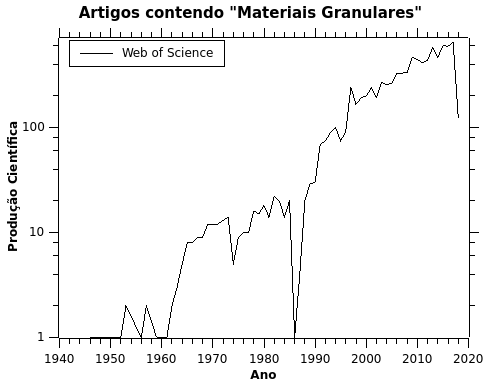
\includegraphics[width=0.8\textwidth]{04-figuras/articles-year.png}
%    \caption{Produção científica acerca de materiais granulares com as palavras chave \textit{"Granular Materials"} ao longo dos anos.}
%    \label{fig:articles-year}
%\end{figure}

\section{Theory}
\label{subsection:Teoria}

%    Como exemplos de materiais granulares temos areia, pedras, solos, fármacos, minérios, alimentos em grãos (arroz, milho, soja, etc.), e até mesmo o cinturão de asteroides e os anéis de Saturno. Só a areia compõe $10\%$ dos materiais da superfície do planeta Terra. Além disso, estima-se que o segundo material mais utilizado nas indústrias são materiais granulares, utilizando aproximadamente $10\%$ de toda a energia do planeta, sendo que o material mais utilizado é a própria água \cite{Sands_Powders_and_Grains}.

    Examples of granular materials includes sand, stones, soils, drugs, ores, grain foods (rice, corn, soybeans, etc.), even the asteroid belt and Saturn's rings. The sand alone makes up $10\%$ of the materials on surface of planet Earth. Besides that, it is estimated that the second most used material in industries are granular materials, using approximately $10\%$ of all the energy on the planet, with the most used material being water itself \cite{Sands_Powders_and_Grains}.

    \begin{figure}
        \begin{minipage}{.45\linewidth}
            \centering
            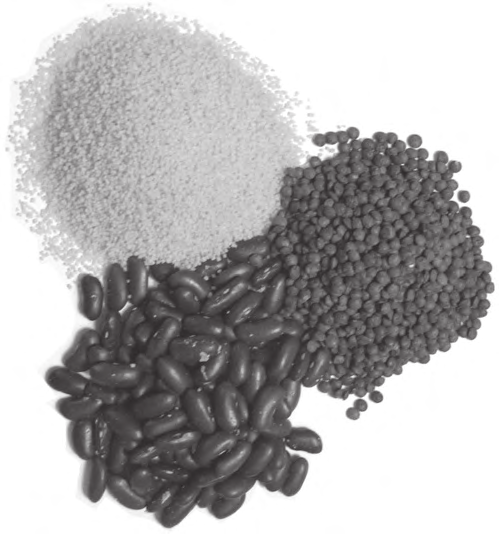
\includegraphics[width=0.9\textwidth]{04-figuras/Exemplo_Alimento.png}
            \subcaption{Grain foods.}
            \label{subfig:exemplo_alimento}
        \end{minipage}
        \begin{minipage}{.45\linewidth}
            \centering
            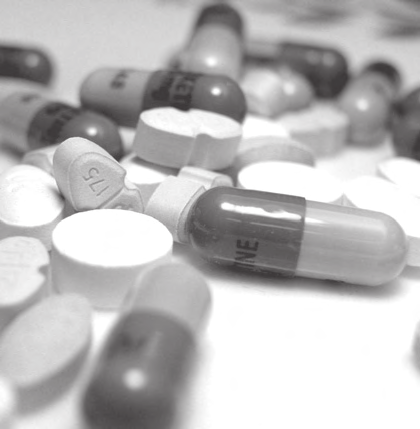
\includegraphics[width=0.9\textwidth]{04-figuras/Exemplo_Medicamento.png}
            \subcaption{Drugs.}
            \label{subfig:exemplo_medicamento}
        \end{minipage}
        \begin{minipage}{.45\linewidth}
            \centering
            \includegraphics[width=0.9\textwidth]{04-figuras/Exemplo_Açucar.png}
            \subcaption{Sugar.}
            \label{subfig:exemplo_acucar}
        \end{minipage}
        \begin{minipage}{.45\linewidth}
            \centering
            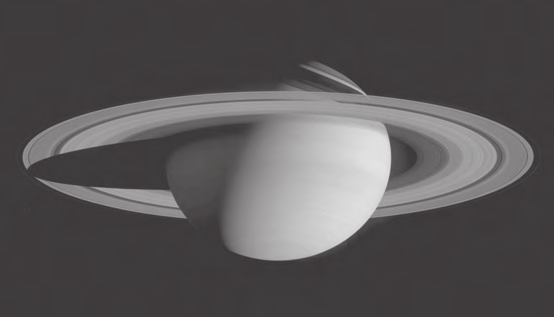
\includegraphics[width=0.9\textwidth]{04-figuras/Exemplo_Saturno.png}
            \subcaption{Saturn and its rings.}
            \label{subfig:exemplo_saturno}
        \end{minipage}
        \caption{Examples of granular material. Figures taken from \cite{Granular_Media_Between_Fluid_and_Solid}.}
    \end{figure}

%    Pela ausência de movimentos Brownianos, bem como pela dissipação de energia, sistemas granulares não sofrem relaxação espontânea de suas configurações estáveis na ausência de perturbações externas, principalmente na forma de vibrações, e portanto não apresentam ergodicidade\footnote{Um sistema ergódico tem característica de transitar entre seus microestados de energia espontaneamente, em intervalos de tempos, implicando que seus estados são todos equiprováveis quando analisados em um longuíssimo tempo \cite{Dissertacao, Srdjan-Tese, Granular_Solids_Liquids_and_Gases}.}.

    Due to the absence of Brownian movements, as well as the dissipation of energy in the contact, granular systems does not undergo spontaneous relaxation of its stable configurations in the absence of external disturbances, and therefore do no have ergodicity\footnote{An ergodic system has the characteristic of moving between their micro-states of energy spontaneously, in intervals of time, implying that their states are all equiprobable when analyzed in a very long time \cite{Srdjan-Tese, Unifying_Concepts_in_Granular_Media_and_Glasses}.}.

    To demonstrate this non-ergodicity, we can think about a dry sand pile that rests at a base. If this base does not oscillate, the structure of the pile does not change, the structure of internal forces will remain unchanged, even if it is heated or cooled. This means that sand grains cannot transit between all equipotential states spontaneously, and than this sand pile will rest with internal configurations (chain-forces, stress tensors, grain contact, etc.) unchanged. In the section \ref{subchap:Fenomenologia}, one can find more details.

%    Materiais granulares apresentam também particularidades quanto às suas fases. Apresentam-se individualmente em corpos sólidos, e quando o conglomerado está próximo do repouso, constituem a fase sólida do sistema. Porém, se o sistema é agitado, ou configurado além de um limiar crítico do ângulo de repouso, pode apresentar-se nas fases de granular líquido\footnote{Granulares líquidos podem possuir uma camada limite que flui sobre a camada sólida do sistema.} ou granular gasoso. Tal classificação ainda está em aberto na literatura, apesar de existirem proposições para o que seria a temperatura granular do sistema \cite{Granular_Solids_Liquids_and_Gases}.

    Granular materials also have particularities regarding their phases, analogously to the state of matter. They are presented individually in solid bodies, and when the conglomerate is close to rest, they constitute the equivalent solid phase of the state of matter. However, if the granular system is slightly agitated, or configured beyond a critical threshold of angle of rest, it can be interpreted in similarity of the liquid state of matter\footnote{Liquid granules can have a boundary layer that flows over the sold layer of the system.}. Granular gases are granular systems that are vigorously agitated, with low packing fraction\footnote{Packing fraction is the measure of the occupied space by the solid portion in relation of the total space.}, and they tend to occupy a large part of the recipe which contains them. An example of the granular state is shown in figure \ref{fig:exemplo_fases}, where the solid phase is static in the bottom, the liquid phase is flowing though layers in the middle, and the gaseous phase is flowing in a higher disordered portion at top. Such classification is still open in the literature, although there are proposals for what would be the granular temperature of the system, in analogous of thermal temperature \cite{Granular_Solids_Liquids_and_Gases}.

    \begin{figure}
        \centering
        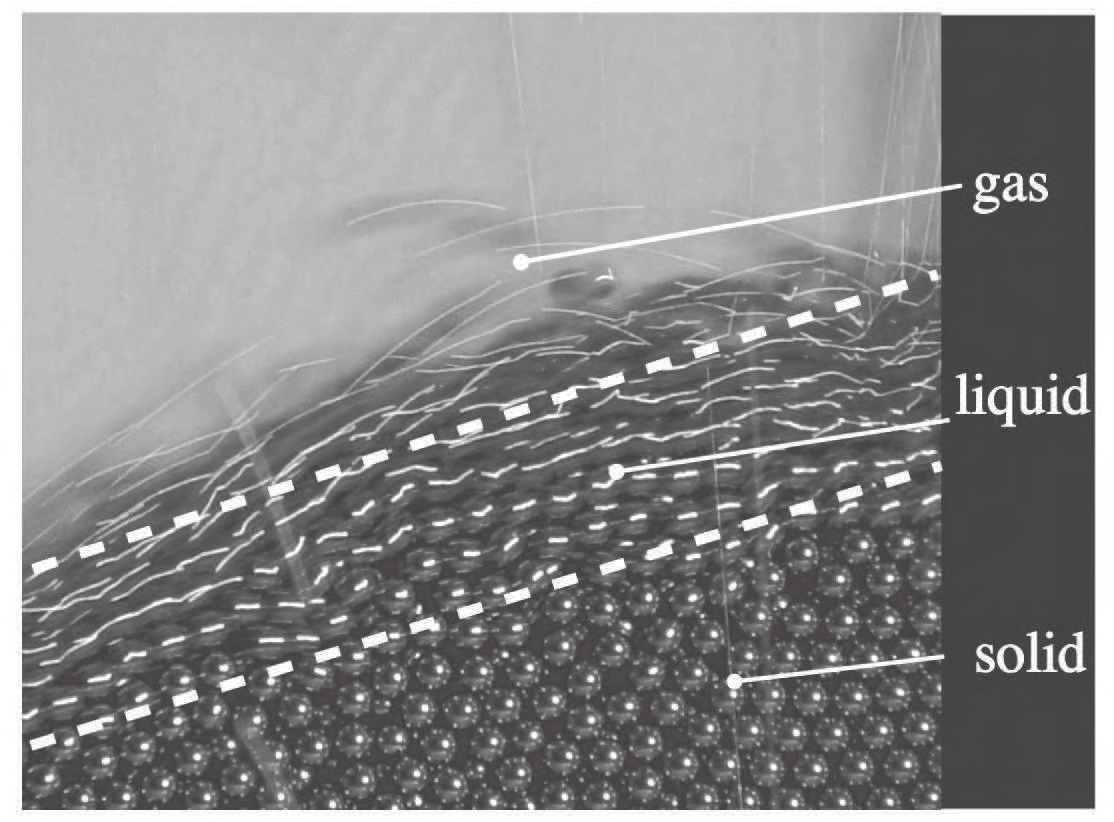
\includegraphics[width=0.9\textwidth]{04-figuras/Exemplo_Fases.png}
        \label{fig:exemplo_fases}
        \caption{Example of three granular phases according their kinetic energy. Figures taken from \cite{Granular_Media_Between_Fluid_and_Solid}.}
    \end{figure}

%    Uma diferenciação entre sistemas granulares pode ser resultado direto das forças de interações entre os grãos. São chamados de granulares secos os sistemas que possuem apenas interações repulsivas, enquanto os granulares molhados apresentam forças de van der Waals nas interações grão a grão. Nesta tese, consideraremos apenas as interações repulsivas de contato, apesar de que em alguns casos, existe fluido envolvendo o material. Consideramos que todo o material que está envolvido pelo mesmo fluido não sofre forças de atração entre os mesmos grãos, e portanto, não está inclusa força de van der Waals na interação entre os grãos.

    A differentiation between granular systems can be a direct result of the interaction forces between grains. Systems that have only repulsive interactions are called dry granulars, while wet granulars have van der Waals forces in grain-to-grain interactions. In this thesis, we will only consider repulsive contact interactions, although in some cases, there is fluid surrounding the material. We consider that all the material that is involved by the same fluid does not suffer forces of attraction between the same grains, and therefore, van der Waals force is not included in the interaction between the grains.

\section{Fenomenologia de Materiais Granulares}
\label{subchap:Fenomenologia}

%Pilha de areia
    Talvez a primeira ideia sobre materiais granulares remeta ao empilhamento de areira. Nesse caso, tem-se uma pilha estática de areia\footnote{A pilha estática está no estado sólido da fase granular \cite{Granular_Solids_Liquids_and_Gases}.}, amontoada sobre uma superfície. Note que em uma pilha como essa, os grãos sempre atingem uma determinada altura, e quando coloca-se mais material sobre a pilha, em algum momento, as camadas superiores da pilha escorrem até a base. Sempre que a pilha ultrapassar o ângulo crítico de repouso \cite{Granular_Physics}, ocorrerá uma avalanche, restaurando o sistema a um outro ângulo característico. Esta propriedade é a de auto-organização\footnote{Um sistema que não possui controlador central, regido por vários agentes que interagem entre si, com regras conhecidas na interação dos agentes e exibem propriedade não prevista pelas interações entre os agentes caracterizam um Sistema Complexo. Uma propriedade característica de Sistemas Complexos e de materiais granulares é a auto-organização. Alguns autores \cite{Mixing_and_Segregation_of_Granular_Materials, Measuring_the_flowing_properties_of_powders_and_grains, Revisiting_localized_deformation_in_sand_with_complex_systems, Granular_matter_and_networks, Patterns_and_collective_behavior_in_granular_media} classificam materiais granulares dentro da área de estudo de Sistemas Complexos.} da pilha de areia pelo ângulo crítico de repouso. Uma boa aproximação do ângulo de repouso é dada pela equação \ref{equ:atrito}:
\begin{equation}
    \label{equ:atrito}
    tan(\theta) = \mu _s ,
\end{equation}
onde $\theta$ é o ângulo crítico de repouso, e $\mu _s$ é o coeficiente de atrito do material.

%Biestabilidade da pilha
    Um pouco mais curioso ainda sobre as pilhas de grãos é que o histórico de preparação do sistema reflete-se no ângulo de repouso \cite{Dynamics_at_the_angle_of_repose}. Este histórico de preparação permite o sistema configurar-se diferentemente, e portanto, o ângulo de repouso assume valores diferentes utilizando o mesmo material. Existe então um ângulo de repouso mínimo $\theta _r$, e um ângulo máximo $\theta _m$, em que o empilhamento pode configurar-se: $\theta _r < \theta < \theta _m$ \cite{Granular_Physics}. Ter uma faixa de ângulos estáveis entre o ângulo mínimo de repouso e o ângulo máximo recebe o nome de biestabilidade do ângulo de repouso.

%Diferentes preparações, diferentes pressões
    Uma evidência de que o histórico de preparação altera a configuração do material é descrita nos artigos "\textit{Sensitivity of Stress Response Function to Packing Preparation}" e "\textit{Memories in sand: Experimental tests of construction history on stress distributions under sandpiles}" \cite{Sensitivity_of_Stress_Response_Function_to_Packing_Preparation, Memories_in_Sand}. A base circular apresentada na figura \ref{fig:pile_stress} foi feita com duas formas de deposição diferentes. No experimento, a pressão medida na base varia de acordo com a deposição, sendo que a deposição feita a partir do funil possui um pico de máximo de pressão em torno de $0,25$ e $0,5$ do raio da mesa, enquanto na deposição feita a partir da peneira apresenta pressão como espécie de platô entre o centro da mesa e $0,25$ do raio, com o máximo próximo do centro.

\begin{figure}
    \centering
    \begin{minipage}{.45\linewidth}
        \centering
        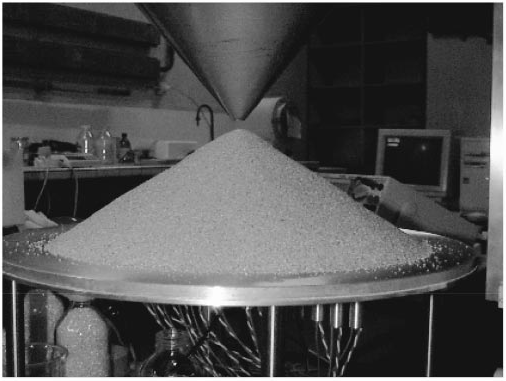
\includegraphics[width=0.9\textwidth]{04-figuras/Sand_Pile_GG_Experiment.png}
        \subcaption{Empilhamento a partir do funil.}
        \label{fig:pressure_pile:GG}
    \end{minipage}
    \begin{minipage}{.45\linewidth}
        \centering
        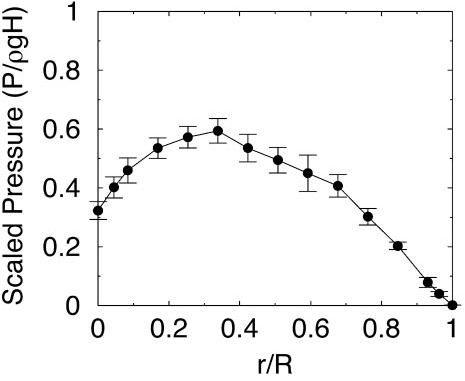
\includegraphics[width=0.9\textwidth]{04-figuras/Sand_Pile_GG_Pressure.png}
        \subcaption{Pressão na montagem a partir do funil.}
        \label{fig:pressure_response:GG}
    \end{minipage}
    \begin{minipage}{.45\linewidth}
        \centering
        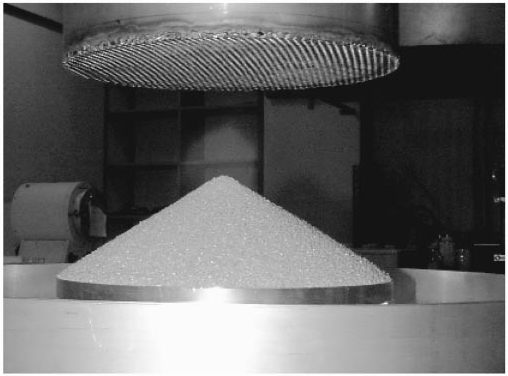
\includegraphics[width=0.9\textwidth]{04-figuras/Sand_Pile_RL_Experiment.png}
        \subcaption{Empilhamento a partir da peneira.}
        \label{fig:pressure_pile:RL}
    \end{minipage}
    \begin{minipage}{.45\linewidth}
        \centering
        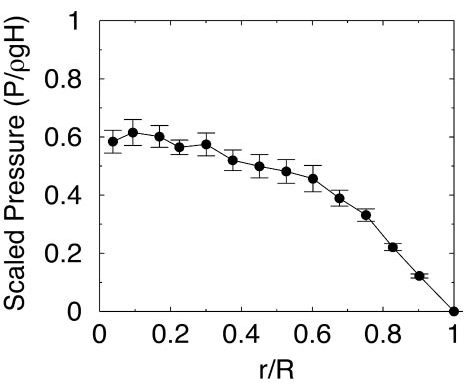
\includegraphics[width=0.9\textwidth]{04-figuras/Sand_Pile_RL_Pressure.png}
        \subcaption{Pressão na montagem a partir da peneira.}
        \label{fig:pressure_response:RL}
    \end{minipage}
    \caption{A preparação das pilhas de areia reflete nas pressões medidas na base da pilha. Nas figuras \ref{fig:pressure_pile:GG} e \ref{fig:pressure_response:GG} a deposição a partir do funil cria um perfil de pressões que tem o pico fora do centro da pilha, enquanto nas figuras \ref{fig:pressure_pile:RL} e \ref{fig:pressure_response:RL} a deposição a partir da peneira cria um perfil de pressões que tem um platô e depois decai. Figuras retiradas de \cite{Memories_in_Sand}.}
    \label{fig:pile_stress}
\end{figure}    

%Função resposta em diferentes configurações
    Um estudo feito por Atman \textit{et al.} \cite{Sensitivity_of_Stress_Response_Function_to_Packing_Preparation} mostra que diferentes geometrias de materiais granulares resultam em diferentes funções respostas\footnote{Função resposta é a diferença entre duas configurações, uma antes de aplicar-se a carga de teste e após a aplicação da carga, mostrando-se a distribuição de forças sobre o material, ou a compressão do sistema \cite{The_Physics_of_Granular_Media}.}. Como exemplo, a figura \ref{fig:stress_response} mostra duas funções respostas para sistemas com geometria circular e pentagonal.

\begin{figure}
    \centering
    \begin{minipage}{.45\linewidth}
        \centering
        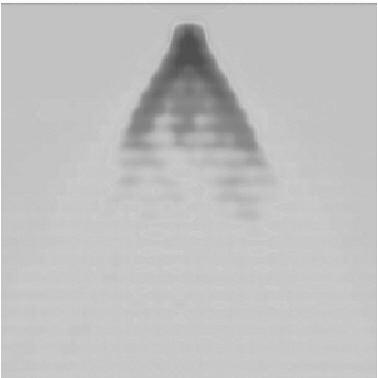
\includegraphics[width=0.9\textwidth]{04-figuras/Funcao_Resposta1.png}
        \subcaption{Grãos circulares.}
        \label{fig:stress_response:circle}
    \end{minipage}
    \begin{minipage}{.45\linewidth}
        \centering
        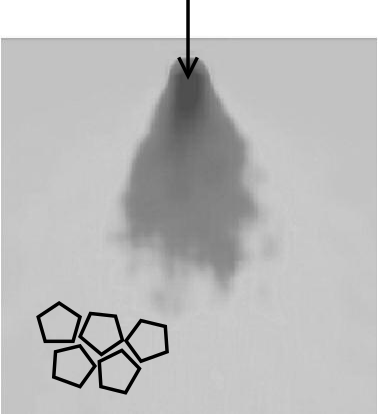
\includegraphics[width=0.9\textwidth]{04-figuras/Funcao_Resposta2.png}
        \subcaption{Grãos pentagonais.}
        \label{fig:stress_response:pentagon}
    \end{minipage}
    \caption{A aplicação de uma força em diferentes sistemas granulares resulta em diferentes funções respostas. A diferença entre estes sistemas é que a figura \ref{fig:stress_response:circle} possui grãos de geometria circular e possui maior ordem, enquanto a figura \ref{fig:stress_response:pentagon} possui geometria pentagonal e maior desordem. Figuras retiradas de \cite{Sensitivity_of_Stress_Response_Function_to_Packing_Preparation}.}
    \label{fig:stress_response}
\end{figure}

%Cadeias de forças em diferentes pilhas
    Já que citamos as diferentes funções respostas nos empilhamentos de grãos, não podemos deixar de citar as cadeias de forças\footnote{Cadeias de forças consistem na rede de contatos entre os grãos que possuem força acima da força média do sistema. Em geral, mede-se as cadeias de forças são medidas a partir da função resposta \cite{The_Physics_of_Granular_Media}.}. A importância experimental da visualização das cadeias de forças se dá no entendimento da distribuição das forças internas que sustentam o material. Como exemplo, a figura \ref{fig:force_chain} indicia a cadeia de forças associada à função resposta de uma força puntual aplicada sobre o topo do material granular.

\begin{figure}
    \centering
    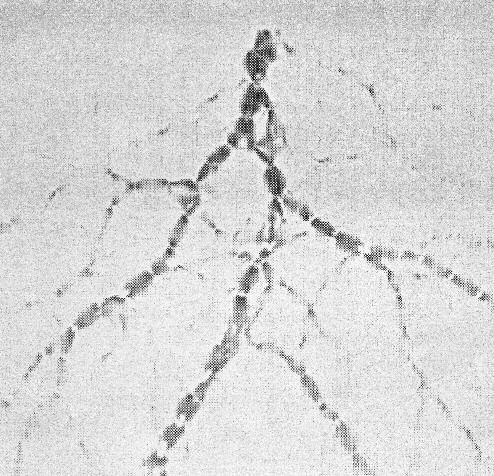
\includegraphics[width=0.5\textwidth]{04-figuras/Cadeia_Forca.png}
    \caption{A aplicação de uma força puntual no topo do material resulta na cadeia de forças, que pode ser vista através da função resposta do sistema. Neste caso, o sistema é preparado com grãos fotoelásticos em uma distribuição bidimensional. Quanto mais escuras, maiores são as tensões no material. Figura retirada de \cite{Sensitivity_of_Stress_Response_Function_to_Packing_Preparation}.}
    \label{fig:force_chain}
\end{figure}

%Formação de arcos
    As cadeias de forças são importantes para entender o fenômeno que está presente nos arcos de sustentação que utilizamos. Arcos são estruturas coletivas que possuem sustentação mútua, e, consequentemente, uma cadeia de forças ligando toda a estrutura, sendo capaz de sustentar o peso próprio e de todos os grãos acima, impedindo que os mesmos escoem. Na formação de arcos podem ocorrer efeitos de segregação, como verificado por Magalhães, C. e Magalhães, F. \cite{Caio-Tese, Felipe-Tese}.

%Pressão e tensão
    As medidas em materiais granulares geralmente tentam caracterizar o material em duas escalas diferentes que se relacionam: microescala, que diz respeito das medidas na escala dos grãos, como atrito; e macroescala, que diz respeito das medidas na escala do sistema, como pressão e tensão de cisalhamento.

%Dilatação
    Uma curiosidade sobre os materiais granulares é que quando estão submetidos a uma pressão e seu coeficiente de compactação\footnote{\label{foot:packingfraction}O coeficiente de compactação é dado pela razão da soma dos volumes individuais dos grãos pelo volume de ocupação no espaço.} está próximo do engarrafamento \cite{Non-Gaussian_behavior_in_jamming_unjamming_transition_in_dense_granular_materials}, uma dilatação tende a ocorrer, expandindo-se pelas bordas das fronteiras que confinam o material ou pelas outras direções de liberdade que o confinamento apresenta. Muitas vezes, ao aplicar-se uma pressão no material confinado, o coeficiente de compactação final pode ser menor que o inicial, indicando uma expansão volumétrica do sistema \cite{Felipe-Tese}.

%Escoamento de granular
    Aproveitando o exemplo do empilhamento, observa-se que na formação da pilha, após os grãos atingem o ângulo critico, ocasiona-se uma avalanche do material. Na avalanche, a camada superior entra em movimento, enquanto as camadas abaixo continuam estáticas. Na movimentação da camada superior, o material granular se apresenta no estado líquido, enquanto a camada estática abaixo encontra-se no estado sólido \cite{Granular_Solids_Liquids_and_Gases}. A figura \ref{fig:inclinacao} exemplifica a transição de fase sólido líquido entre as camadas.

\begin{figure}
    \centering
    \begin{minipage}{.45\linewidth}
        \centering
        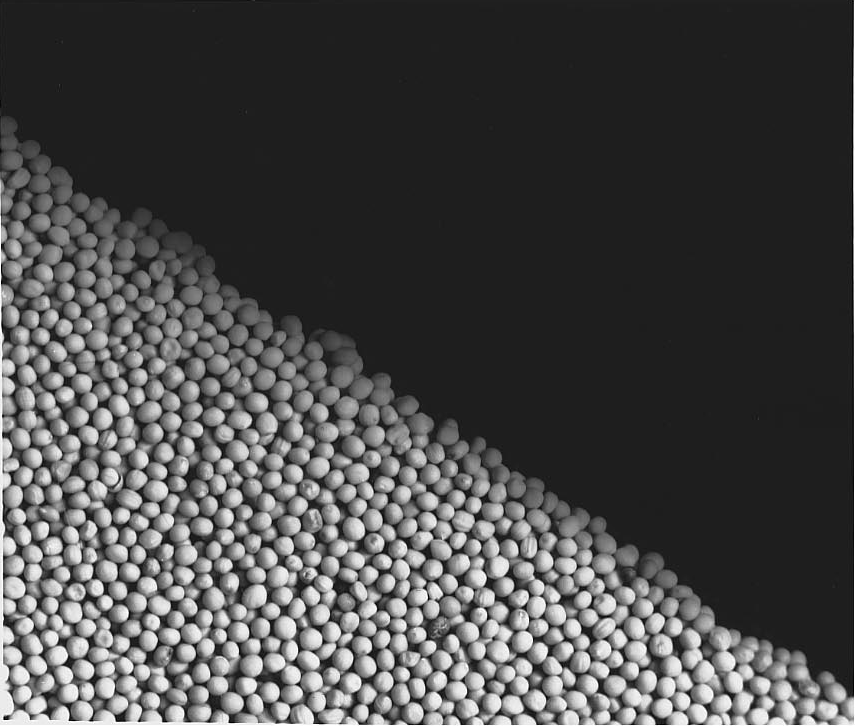
\includegraphics[width=0.9\textwidth]{04-figuras/Pilha1.png}
        \subcaption{Pilha estática.}
        \label{fig:inclinacao:solido}
    \end{minipage}
    \begin{minipage}{.45\linewidth}
        \centering
        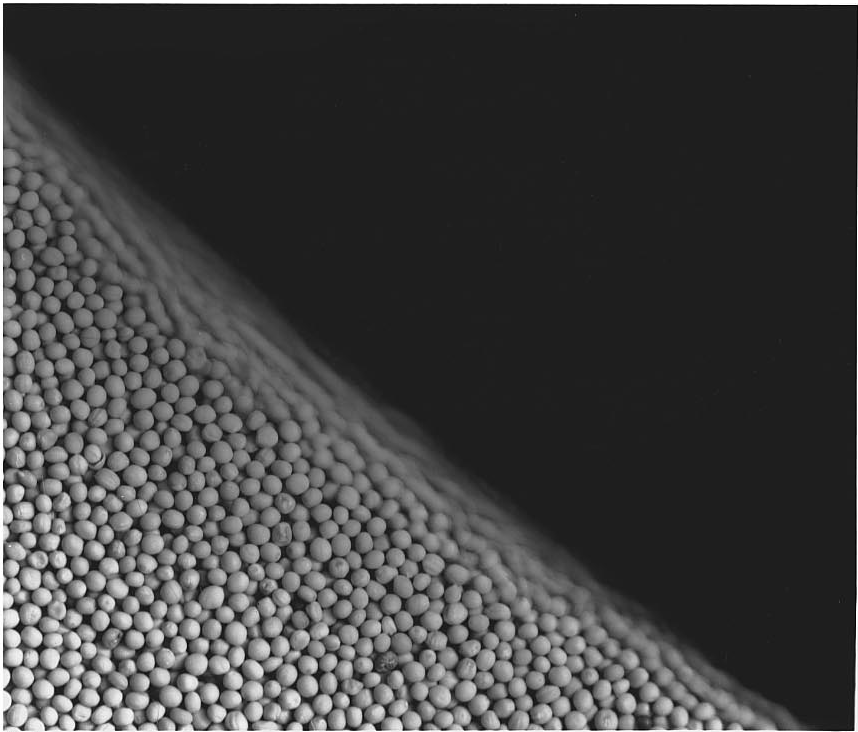
\includegraphics[width=0.9\textwidth]{04-figuras/Pilha2.png}
        \subcaption{Pilha escorrendo.}
        \label{fig:inclinacao:liquido}
    \end{minipage}
    \caption{Com o aumento do ângulo da pilha, nota-se que a camada superior desliza sobre a camada inferior (da figura \ref{fig:inclinacao:solido} para a figura \ref{fig:inclinacao:liquido}). Figuras retiradas de \cite{Granular_Solids_Liquids_and_Gases}.}
    \label{fig:inclinacao}
\end{figure}

    Escoamentos podem ocorrer então por tensões aplicadas no material, seja em uma inclinação da base, seja pela vibração do material. Como a mudança de configurações do material está relacionada a taxa de cisalhamento do material, mas a tensão de cisalhamento não é necessariamente proporcional a taxa de cisalhamento, este escoamento pode ser classificado como fluido não newtoniano.

%Segregação
%    Um fenômeno muito estudado é a segregação dos materiais granulares. O efeito de segregação ocorre em diferentes geometrias de material, densidades e coeficientes de atrito.

%Vibração
%    Vibrações no material granular fornecem energia ao sistema

    No próximo capítulo descreveremos as equações e os procedimentos para realizar as simulações dos materiais granulares, desde o modelo de contatos até a inserção do fluido no sistema.
    % Trabalhos relacionados
\chapter{Metodologia}
\label{chap:DEM}
    Uma forma muito utilizada para estudar sistemas granulares é a realização de simulações numéricas, que têm um papel importante na complementação das informações experimentais, o que aumenta ainda mais a compreensão dos fenômenos da física granular. Uma justificativa é o controle preciso dos parâmetros de entrada das simulações e do nível de complexidade acerca do objeto de estudo. Outra vantagem é a facilidade da medição próxima da escala dos grãos, como as cadeias de forças, até a escala do sistema, como o cisalhamento do material, evidenciando eventuais propriedades emergentes e suas causas.

    A técnica de simulação de materiais granulares que utilizamos neste trabalho é um \textit{DEM} conhecido na literatura como Dinâmica Molecular, ou \textit{Molecular Dynamics (MD)}. O método consiste em solucionar numericamente as equações de movimento quando aplicadas forças dinâmicas sobre os elementos a serem simulados. Uma vantagem deste método é que qualquer força que utilize parâmetros dentro da simulação e que possa ser descrita na interação com os elementos é aceita neste método.

    A técnica descrita no livro \textit{Computer Simulation of Liquids} \cite{Computer_Simulation_of_Liquids} utiliza-se dos formalismos da mecânica analítica através dos potenciais de interação entre os agentes, sejam potenciais lagrangianos, sejam potenciais hamiltonianos, para estabelecer a força que atua sobre cada agente. A desvantagem deste tipo de descrição é que forças dissipativas podem não aparecer, uma vez que a descrição das forças está relacionada diretamente com potenciais. Formalmente, o sistema deve obedecer ao conjunto de equações \ref{equ:lagrange} descritas pela função lagrangiana do sistema:
\begin{subequations}
    \label{equ:lagrange}
    \begin{empheq}[left={}]{align}
        \label{equ:lagrange1}
        \mathcal{L} &= \mathcal{T} - \mathcal{V},\\
        \label{equ:lagrange2}
        \sum_{k} \left[\frac{d}{dt} \left( \frac{\partial \mathcal{L}}{\partial \dot{q_k}} \right) - \left(\frac{\partial \mathcal{L}}{\partial q_k} \right)\right] &= 0,\\
        \label{equ:lagrange_forca}
        \vec{F}_{i} = \nabla \mathcal{L} &= -\nabla \mathcal{V},
    \end{empheq}
\end{subequations}
sendo que a notação descrita pelo conjunto de equações \ref{equ:lagrange}, $\mathcal{L}$ representa a função lagrangiana que rege a dinâmica do sistema, $\mathcal{T}$ a energia cinética, $\mathcal{V}$ a energia potencial, $k$ o número de coordenadas generalizadas do sistema, $q_{k}$ as coordenadas generalizadas, $\dot{q_{k}}$ as velocidades generalizadas, $\overrightarrow{F_{i}}$ a força exercida na partícula $i$ originada pelo gradiente do potencial $\mathcal{V}$.

    Já outras referências \cite{Dissertacao, Abraao-Dissertacao, Caio-Dissertacao, Caio-Tese, Bouzid-Tese, Wassgren-Tese, Felipe-Tese, Srdjan-Tese, Luding-Tese, Computational_Granular_Dynamics} utilizam o modelo diretamente das forças que agem sobre cada elemento.

\section{Equações de movimento}
    Para a realização da simulação, o conjunto de equações \ref{equ:movimento} deve ser satisfeito, o que leva em consideração as leis de Newton. Assim, tem-se a informação dos estados dos agentes em função do tempo.
\begin{subequations}
    \label{equ:movimento}
    \begin{empheq}[left={Translacional}\empheqlbrace]{align}
        \label{equ:posicao_linear}
        \vec{r}_{i}(t) &= \vec{r}_{i}(0) + \int_{0}^{t} \vec{v}_{i}(t) dt,\\
        \label{equ:velocidade_linear}
        \vec{v}_{i}(t) &= \vec{v}_{i}(0) + \int_{0}^{t} \vec{a}_{i}(t) dt,\\
        \label{equ:aceleracao_linear}
        \vec{a}_{i}(t) &= \sum_{j} \frac{\vec{F}_{i,j}(t)}{m_{i}},
    \end{empheq}
    \begin{empheq}[left={Rotacional}\empheqlbrace]{align}
        \label{equ:posicao_angular}
        \theta^{k}_{i}(t) &= \theta^{k}_{i}(0) + \int_{0}^{t} \vec{\omega}^{k}_{i}(t) dt,\\
        \label{equ:velocidade_angular}
        \vec{\omega}^{k}_{i}(t) &= \vec{\omega}^{k}_{i}(0) + \int_{0}^{t} \vec{\alpha}^{k}_{i}(t) dt,\\
        \label{equ:aceleracao_angular}
        \vec{\alpha}^{k}_{i}(t) &= {I^{k}_{i}}^{-1} \sum_{j} \vec{\tau}^{k}_{i,j}(t),
    \end{empheq}
\end{subequations}
em que $i$ é a i-ésima partícula do sistema, $\vec{r}_{i}(t)$ é o vetor de posição do centro de massa do corpo $i$ no instante de tempo $t$, $\vec{v}_{i}(t)$ ou $\vec{\dot{r}}_{i}(t)$ é o vetor de velocidade do centro de massa do corpo, $\vec{a}_{i}(t)$ ou $\vec{\dot{v}}_{i}(t)$ ou $\vec{\ddot{r}}_{i}(t)$ é o vetor de acelerações do centro de massa do corpo, $\vec{F}_{i,j}(t)$ é a componente da força que o centro de massa do corpo sofre por interagir com outro corpo ou campo $j$, $m_{i}$ é a massa do corpo, $\theta^{k}_{i}(t)$ é a base das coordenadas de rotação do corpo expressas na base $k$ do sistema, $\vec{\omega}^{k}_{i}(t)$ é o pseudovetor de velocidades angulares do corpo expressas na base $k$ do sistema, $\vec{\alpha}^{k}_{i}(t)$ é o pseudovetor de acelerações angulares do corpo, ${I^{k}_{i}}^{-1}$ é o inverso do tensor de inércia do corpo e $\vec{\tau}^{k}_{i,j}(t)$ é o vetor de torques que o corpo sofre por interagir com outro corpo ou campo. Lembrando que a relação entre o torque e a força que o causa pode ser descrita pela equação \ref{equ:torque}:
\begin{equation}
    \label{equ:torque}
    \vec{\tau}_{i,j}(t) = \vec{\chi}_{i,j}(t) \times \vec{F}_{i,j}(t),
\end{equation}
sendo que o vetor $\vec{\tau}_{i,j}(t)$ é o produto vetorial entre o vetor $\vec{\chi}_{i,j}(t)$, que liga o centro de massa da partícula $i$ ao ponto de aplicação da força, e o vetor $\vec{F}_{i,j}(t)$, o vetor da força causada por interagir com outro corpo ou campo $j$. As equações \ref{equ:aceleracao_linear} e \ref{equ:aceleracao_angular} expressam a segunda lei de Newton.

    A formulação descrita pelo conjunto de equações \ref{equ:movimento} abrange espaços em 1D, 2D e 3D, porém esta tese foca apenas na formulação de sistemas em 2D.

\subsection{Modelo de forças}
\label{subchap:Modelo_Forcas}
    As forças presentes nos sistemas modelados nesta tese incluem as forças de contato entre os agentes, que pertencem ao modelo reológico dos grãos, as forças de interação entre grão e fluido e a força gravitacional.

\subsubsection{Modelo reológico}
\label{subsubchap:Reologia}
    O modelo reológico dos agentes utilizado na simulação de \textit{MD} para materiais granulares foi proposto por Kelvin-Voigt \cite{Dissertacao}, com geometria circular pelos agentes. A reologia de Kelvin-Voigt modela a força de contato por uma mola e um amortecedor em paralelo na direção normal do contato, como exemplificado na figura \ref{fig:forcas}. A parcela da mola representa a contribuição elástica do material, relacionado com o módulo de Young, enquanto o amortecedor tem a função de atenuar a energia na colisão inelástica entre os grãos. Adicionalmente, um elemento parecido com uma mola é inserido na direção tangencial. Um modelo proposto em \cite{Caio-Tese} adiciona um elemento parecido com um amortecedor em paralelo à mola tangencial, modelando a resistência ao rolamento. Por causa da geometria circular, toda a variação de momento angular é causada pela força tangencial.

\begin{figure}
    \begin{minipage}{.45\linewidth}
        \centering
        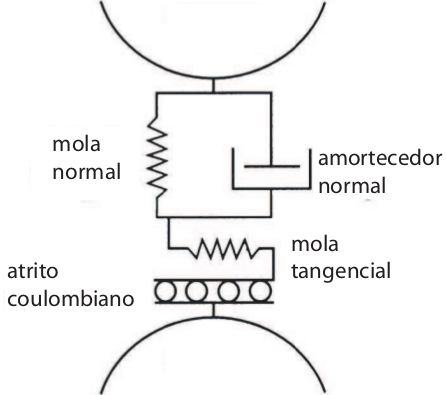
\includegraphics[width=0.9\textwidth]{04-figuras/Modelo_Forcas.png}
        \subcaption{Modelo de forças de contato entre os agentes.}
        \label{fig:forcas_modelo}
    \end{minipage}
    \begin{minipage}{.45\linewidth}
        \centering
        \includegraphics[width=0.9\textwidth]{04-figuras/Contato.tikz}
        \subcaption{Aplicação do contato entre os agentes.}
        \label{fig:forcas_contato}
    \end{minipage}
    \caption{Modelo de forças e a aplicação do contato entre os agentes. Figuras retiradas de \cite{Dissertacao}.}
    \label{fig:forcas}
\end{figure}

    Uma peculiaridade da \textit{MD} é a permissão de interpenetração entre os grãos, e portanto, neste modelo não há deformação no contato entre dois corpos. A interpenetração máxima é controlada pelo parâmetro de dureza do material e impondo penetração de $0.5\%$ dos raios.

    Para encontrar o valor da interpenetração $\delta$, na geometria circular, a equação \ref{equ:interpenetracao}:
\begin{equation}
    \label{equ:interpenetracao}
    \delta_{i,j}^{\perp} = \left(R_{i}+R_{j}-\left|\vec{r}_{j}-\vec{r}_{i}\right|\right)\mathcal{H}(R_{i}+R_{j}-\left|\vec{r}_{j}-\vec{r}_{i}\right|),
\end{equation}
em que $\delta_{i,j}^{\perp}$ é o valor da interpenetração entre os grãos $i$ e $j$, $R_{i}$ é o raio do corpo $i$, $R_{j}$ do corpo $j$, $\vec{r}_{i}$ é o vetor de posição do corpo $i$, $\vec{r}_{j}$ é o vetor de posição do corpo $j$ e $\mathcal{H}$ é a função de degrau de Heaviside. Então, quando a distância entre os corpos for maior que a soma dos raios, os corpos não estarão em contato e a função degrau de Heaviside indica que a interpenetração entre os grãos é nula.

    Com o contato entre os grãos, a consequência direta da interpenetração é o surgimento de uma força elástica repulsiva ao contato, e dependente da função de interpenetração $\delta^{\perp}$. A expressão da força pode ser calculada pela equação \ref{equ:forca_elastica}:
\begin{equation}
    \label{equ:forca_elastica}
    \vec{F}_{i,j}^{el} = -k_{n}\left(\delta_{i,j}^{\perp}\right)^{\frac{D}{2}}\hat{n}_{i,j},
\end{equation}
em que $\vec{F}_{i,j}^{el}$ é a força elástica que o corpo $i$ sente ao entrar em contato com o corpo $j$, $k_{n}$ é a constante relacionada a elasticidade do material na direção do contato, $\delta_{i,j}^{\perp}$ é a interpenetração entre os corpos $i$ e $j$, $D$ é a dimensão do sistema (no caso, $D=2$) e $\hat{n}_{i,j}$ é a direção normal do contato \cite{Dissertacao, Caio-Tese, Landau}. Pode-se escrever um potencial para esta força elástica como: $\mathcal{V} = \frac{1}{2}k_{n}{\delta_{i,j}^{\perp}}^2$.

    Associado à força elástica, também está presente a força de amortecimento. Por se tratar de uma força dissipativa, não se pode associar um potencial à força de amortecimento. A maior parcela da perda de energia dos materiais granulares está na colisão, e esta é a responsável. A equação \ref{equ:forca_amortecimento} descreve seu comportamento:
\begin{equation}
    \label{equ:forca_amortecimento}
    \vec{F}_{i,j}^{am} = -\gamma \left(\vec{v}_{i,j}.\hat{n}_{i,j}\right)\hat{n}_{i,j},
\end{equation}
em que $\vec{F}_{i,j}^{am}$ é a força de amortecimento que o corpo $i$ sente ao entrar em contato com o corpo $j$, $\gamma$ é a constante de amortecimento relacionada a inelasticidade da colisão, $\vec{v}_{i,j}$ é a velocidade relativa entre os centros de massa dos corpos $i$ e $j$ e e $\hat{n}_{i,j}$ é a direção normal do contato \cite{Dissertacao, Caio-Tese, Computational_Granular_Dynamics}.

    A constante de amortecimento está diretamente ligada ao coeficiente de restituição e pode ser utilizada equivalentemente através da transformação mostrada em \cite{Dissertacao}. Alguns autores utilizam o coeficiente de restituição nas simulações, como \cite{Computational_Granular_Dynamics, Luding-Tese, Srdjan-Tese}. Aqui, utilizaremos a constante de amortecimento.

    A força de atrito também está presente no modelo de simulação. Como as superfícies estão em contato, existirá uma força de atrito entre elas, se houver tendência de movimento uma em relação à outra. Em especial, devido à geometria circular, as forças de atrito agirão apenas na direção tangencial. A velocidade de deslocamento entre os pontos de contato dos corpos é dada pela equação \ref{equ:velocidade_relativa} a seguir:
\begin{equation}
  \label{equ:velocidade_relativa}
  \delta_{i,j}^{\parallel} = \vec{v}_{ij}.\hat{t}_{ij} - R_{i}\omega_{i} - R_{j}\omega_{j},
\end{equation}
em que $\delta_{i,j}^{\parallel}$ é a velocidade relativa entre os pontos de contato dos corpos $i$ e $j$, $\vec{v}_{ij}$ é a velocidade relativa entre os centros de massa dos corpos $i$ e $j$, $\hat{t}_{ij}$ é o vetor tangencial às superfícies de contato dos corpos $i$ e $j$, $R_{i}$ é o raio do corpo $i$, $R_{j}$ é o raio do corpo $j$, $\omega_{i}$ é a velocidade de rotação do corpo $i$ e $\omega_{j}$ é a velocidade de rotação do corpo $j$.

    Para a força tangencial, é necessário saber o deslocamento relativo dos pontos de contato, como dada pela equação \ref{equ:velocidade_relativa}, aplicados no sistema de equações \ref{equ:forca_atrito}, que modela a força de atrito com saturação, e é dada por:
\begin{equation}
    \label{equ:forca_atrito}
    \vec{F}_{i,j}^{at} = \left\{
    \begin{array}{l l l}
        \displaystyle -\int_{t_{0}}^{t_{f}} k_{t} \delta_{i,j}^{\parallel} \hat{t}_{ij}\, \mathrm{d} t, & \quad \textrm{se } k_{t} \left| \delta_{i,j}^{\parallel} \right| \leq \mu \left|F_{i,j}^{n}\right| & \textrm{ (Atrito Estático)} \\
        \displaystyle -\int_{t_{0}}^{t_{f}} \frac{\delta_{i,j}^{\parallel}}{\left|\delta_{i,j}^{\parallel}\right|} \mu \left| F_{i,j}^{n} \right| \hat{t}_{ij}\, \mathrm{d} t, & \quad \textrm{se } k_{t} \left| \delta_{i,j}^{\parallel} \right| > \mu \left| F_{i,j}^{n} \right| & \textrm{ (Atrito Cinético)}
    \end{array}
    \right.\ ,
\end{equation}
em que $\vec{F}_{i,j}^{at}$ é a força de atrito entre os corpos $i$ e $j$, $k_{t}$ é a constante elástica do material na direção tangencial, $\delta_{i,j}^{\parallel}$ é a velocidade relativa entre os pontos de contato dos corpos $i$ e $j$, $\hat{t}_{ij}$ é o vetor tangencial às superfícies de contato dos corpos $i$ e $j$, $\mu$ é o coeficiente de atrito entre as superfícies dos corpos $i$ e $j$ e $\vec{F}_{i,j}^{n} = \vec{F}_{i,j}^{el} +\vec{F}_{i,j}^{am}$ é a força normal às superfícies dos corpos $i$ e $j$.

\subsubsection{A força externa: Gravidade}
\label{subsubchap:Gravidade}
    Para este modelo, a influência gravitacional é aproximada por uma constante, já que a simulação não leva em conta que a influência da massa dos corpos é muito pequena, se comparada com a massa do planeta em que está situada a simulação, bem como a variação de altura do sistema simulado é muito pequeno e está próximo à superfície do planeta, quando comparada com o raio do planeta. Por conveniência, normalizamos a gravidade como valor unitário.

\subsubsection{As forças do fluido}
\label{subsubchap:Fluido}
    A força que o fluido exerce sobre os corpos pode ser entendida como contribuição de diferentes modelos e casos. Uma formulação mais detalhada sobre cada parcela de forças que o fluido exerce sobre cada corpo é descrita pela equação \ref{equ:forcas_fluido}:
\begin{equation}
    \label{equ:forcas_fluido}
    \vec{F}_{i}^{Fluid} = \vec{F}_{i}^{Arch} +\vec{F}_{i}^{Drag} +\vec{F}_{i}^{Magnus} +\vec{F}_{i}^{Lift} +\vec{F}_{i}^{AddedMass} +\vec{F}_{i}^{Basset},
\end{equation}
em que $\vec{F}_{i}^{Fluid}$ é a contribuição total das forças que o fluido exerce sobre o corpo $i$, $\vec{F}_{i}^{Arch}$ é a força de Arquimedes sobre o corpo $i$, $\vec{F}_{i}^{Drag}$ é a força de arrasto sobre o corpo $i$, $\vec{F}_{i}^{Magnus}$ é a força de Magnus sobre o corpo $i$, $\vec{F}_{i}^{Lift}$ é a força de sustentação sobre o corpo $i$, $\vec{F}_{i}^{AddedMass}$ é a força de adição de massa sobre o corpo $i$ e $\vec{F}_{i}^{Basset}$ é a força histórica de Basset sobre o corpo $i$. Como simplificação do modelo, utilizaremos apenas as forças de Arquimedes e as forças de arraste do fluido \cite{Fluid_Mechanics, Numerical_simulation_of_turbulent_sediment_transport, Maurin-Tese}.

    A força de Arquimedes pode ser escrita como na equação \ref{equ:arquimedes}, enquanto a força de arraste pode ser escrita como na equação \ref{equ:arraste}:
\begin{equation}
    \label{equ:arquimedes}
    \vec{F}_{i}^{Arch} = \frac{\pi}{6} d_{i}^{3} \vec{\nabla}.\overline{\overline{\sigma}},
\end{equation}
em que $\vec{F}_{i}^{Arch}$ é a força de Arquimedes no corpo $i$, $d_{i}$ é o diâmetro do corpo $i$ e $\vec{\nabla}.\overline{\overline{\sigma}}$ é o divergente do tensor de tensão do fluido $\overline{\overline{\sigma}}$, e:
\begin{equation}
    \label{equ:arraste}
    \vec{F}_{i}^{Drag} = \frac{\pi}{8}\rho_{f}d_{i}^{2}C_{d}(\mathcal{R}_{u})\left|\vec{u}_{f}-\vec{v}_{i}\right|(\vec{u}_{f}-\vec{v}_{i}),
\end{equation}
em que $\vec{F}_{i}^{Drag}$ é a força de arraste no corpo $i$, $\rho_{f}$ é a densidade do fluido, $d_{i}$ é o diâmetro do corpo $i$, $C_{d}(\mathcal{R}_{u})$ é o coeficiente de arrasto em função do número de Reynolds do corpo, descrito pela equação \ref{equ:reynolds_arraste}, $\vec{u}_{f}$ é a velocidade do fluido, $\vec{v}_{i}$ é a velocidade do corpo \cite{Numerical_simulation_of_turbulent_sediment_transport}.

\begin{equation}
    \label{equ:reynolds_arraste}
    C_{u}(\mathcal{R}_{u}) = \left( \sqrt{C_{d}^{\infty}} +\sqrt{\frac{\mathcal{R}_{u}^{c}}{\mathcal{R}_{u}}} \right)^{2}
\end{equation}
em que $C_{u}(\mathcal{R}_{u})$ é o coeficiente de arrasto em função do número de Reynolds do corpo, $C_{d}^{\infty} \simeq 0.5$ é o coeficiente de arrasto do grão no limite turbulento ($\mathcal{R}_{u} \to \infty$), $\mathcal{R}_{u}^{c} \simeq 24$ é o número de Reynolds de transição do corpo na qual o coeficiente de arrasto torna-se quase constante e a equação \ref{equ:reynolds_fluido_grao} que relaciona o número de Reynolds do corpo com os parâmetros do sistema:
\begin{equation}
    \label{equ:reynolds_fluido_grao}
    \mathcal{R}_{u} = \frac{d_{i}}{\nu} \left| \vec{u}_{f} -\vec{v}_{i} \right|
\end{equation}
em que $d_{i}$ é o diâmetro do corpo $i$, $\nu$ é a viscosidade dinâmica do sistema, $\vec{u}_{f}$ é a velocidade do fluido e $\vec{v}_{i}$ é a velocidade do corpo $i$ \cite{Numerical_simulation_of_turbulent_sediment_transport}.

\subsection{O modelo do fluido}
    Para o fluido, a equação geral que rege o sistema é a equação de Navier-Stokes, que é a aplicação da segunda lei de Newton para a massa específica em meios contínuos e a aplicação das leis de conservação de massa e de momento \cite{Physical_Hydrodynamics, Fluid_Mechanics}. Para a equação da conservação de massa, temos a equação \ref{equ:conservacao_massa}:
\begin{equation}
    \label{equ:conservacao_massa}
    \frac{\partial \rho^{f}}{\partial t} +\vec{\nabla}.(\rho \vec{u}^{f}) = 0,
\end{equation}
em que $\rho^{f}$ é a densidade do fluido, e $\vec{u}^{f}$ é a velocidade do fluido.

    A equação \ref{equ:conservacao_momento} descreve a conservação do momento como:
\begin{equation}
    \label{equ:conservacao_momento}
    \frac{\partial}{\partial t}\left(\rho^{f}\vec{u}^{f}\right) +\vec{\nabla}.\left(\rho^{f}\vec{u}^{f}\otimes\vec{u}^{f}\right) = \overline{\overline{\sigma}} +p_{ext},
\end{equation}
em que $\rho^{f}$ é a densidade do fluido, $\vec{u}^{f}$ é a velocidade do fluido, $\overline{\overline{\sigma}}$ é o tensor tensão do fluido e $p_{ext}$ é a pressão causada por agentes externos, como a gravidade e as forças dos corpos que interagem com o fluido.

    Na formulação da conservação do momento, existe internamente a conservação da massa, e se escrevermos os termos da equação efetuando-se os produtos internos e as derivadas, teremos a equação \ref{equ:Navier-Stokes}, que é a equação de Navier-Stokes:
\begin{equation}
    \label{equ:Navier-Stokes}
    \rho^{f} \frac{\partial \vec{u}^{f}}{\partial t} +\rho^{f}\left(\vec{u}^{f}.\vec{\nabla}\right)\vec{u}^{f} = \vec{\nabla}.\overline{\overline{\sigma}} +p_{ext},
\end{equation}
em que $\rho^{f}$ é a densidade do fluido, $\vec{u}^{f}$ é a velocidade do fluido, $\overline{\overline{\sigma}}$ é o tensor tensão do fluido e $p_{ext}$ é a pressão causada por agentes externos e que o tensor tensão do fluido pode ser escrito em função das pressões internas e do cisalhamento do fluido, como na equação \ref{equ:tensor_tensao}:
\begin{equation}
    \label{equ:tensor_tensao}
    \overline{\overline{\sigma}} = \left(
    \begin{matrix}
        \sigma_{xx} & \tau_{xy} \\
        \tau_{yx} & \sigma_{yy}
    \end{matrix}
    \right),
\end{equation}
em que $\overline{\overline{\sigma}}$ é o tensor de tensão do fluido, $\sigma$ são as componentes de tensão e a pressão do fluido é $p=-\frac{1}{2}(\sigma_{xx}+\sigma_{yy})$, e $\tau$ são as componentes do cisalhamento do fluido, sendo que $\tau_{xy} = \tau{yx}$, indicando que são simétricas.

    Uma importante medida é a taxa de deformação do fluido, dada pela equação \ref{equ:taxa_deformacao}:
\begin{equation}
    \label{equ:taxa_deformacao}
    \dot{\gamma}_{xy} = \frac{1}{2} \left(\frac{\partial u_{x}}{\partial y} +\frac{\partial u_{y}}{\partial x} \right),
\end{equation}
em que $\dot{\gamma_{xy}}$ e $\dot{\gamma_{yx}}$ são as componentes do tensor da taxa de deformação, $u_{x}$ é a velocidade do fluido na direção de escoamento e $u_{y}$ é a velocidade do fluido na direção da gravidade. As componentes $\dot{\gamma_{xy}}$ e $\dot{\gamma_{yx}}$ são simétricas, sendo também equivalentes às componentes cruzadas do divergente do campo de velocidades.

    O cisalhamento do fluido controla algumas características do fluido, como por exemplo o regime de escoamento. A equação que rege o cisalhamento é a equação \ref{equ:cisalhamento}:
\begin{equation}
    \label{equ:cisalhamento}
    \tau = \rho^{f}(\nu+\nu_{t})\dot{\gamma},
\end{equation}
em que $\tau$ é cisalhamento do fluido, $\rho^{f}$ é a densidade do fluido, $\nu$ é a viscosidade intrínseca do fluido, $\nu_{t}$ é a viscosidade que insere turbulência no fluido e $\dot{\gamma}$ é o tensor da taxa de deformação do fluido e é descrito pela equação \ref{equ:taxa_deformacao}. Para que o escoamento seja laminar em um fluido newtoniano, o termo de viscosidade turbulenta deve ser nulo.

    As considerações feitas sobre o fluido são que o fluido é incompressível, que o fluido não circula na direção da gravidade (direção $x$ de escoamento), que possui condição periódica de contorno na direção de escoamento, ou seja, o que acontece de um lado do sistema é o mesmo que acontece no outro e o volume ocupado pelo fluido é o todo o volume não ocupado pelos corpos. As implicações destas condições simplificam as equações \ref{equ:conservacao_massa}, \ref{equ:conservacao_momento} e \ref{equ:Navier-Stokes}. No caso da conservação da massa a implicação da incompressibilidade do fluido é a conservação do volume ao longo de todo o tempo e todo o espaço. Já a condição periódica de contorno na direção do escoamento, em relação à  Navier-Stokes, equação \ref{equ:Navier-Stokes}, implica que a tensão na direção de escoamento seja nula, ou seja, $\sigma_{xx} = 0$ quando não houverem corpos. Para o fluido não circular na direção da gravidade, toda a camada de escoamento é tomada por uma média na direção do escoamento (direção $x$). Portanto, a simplificação do tensor de tensões do fluido resume-se na equação \ref{equ:divergente_tensor_tensao}:
\begin{equation}
    \label{equ:divergente_tensor_tensao}
    \vec{\nabla}.\overline{\overline{\sigma}} = \frac{\partial \tau}{\partial y} \hat{x} - \frac{\partial p}{\partial y} \hat{y}
\end{equation}
em que $\overline{\overline{\sigma}}$ é o tensor de tensão do fluido, $\tau$ é a componente do cisalhamento do fluido, $p$ é componente da pressão do fluido, $\hat{x}$ é a direção de escoamento do fluido e $\hat{y}$ é a direção da gravidade.

    Aplicando as considerações feitas sobre o fluido na equação de Navier-Stokes, equação \ref{equ:Navier-Stokes}, tem-se o sistema de equações em relações às direções de escoamento do fluido ($x$) e da gravidade ($y$) iguais a:
\begin{subequations}
    \label{equ:fluido}
    \begin{empheq}[left={}\empheqlbrace]{align}
        \label{equ:fluido_x}
        (1-\phi) \rho^{f} \frac{\partial u_{x}^{f}}{\partial t} &= (1-\phi) \frac{\partial \tau}{\partial y} - p_{x}^{body} & : \hat{x},\\
        \label{equ:fluido_y}
         0 &= -(1-\phi) \frac{\partial \sigma_{yy}}{\partial x} - p_{y}^{body} + (1-\phi)\rho^{f}g & : \hat{y},
    \end{empheq}
\end{subequations}
em que $\rho^{f}$ é a densidade do fluido, $u_{x}^{f}$ é a componente da velocidade na direção do escoamento, $\phi$ é o coeficiente de compactação dos corpos, $\tau$ é a componente do cisalhamento do fluido, $\sigma_{yy}$ é a componente da tensão no fluido, $p_{x}^{body}$ é a pressão que os corpos fazem sobre a direção de escoamento $x$, $p_{y}^{body}$ é a pressão que os corpos fazem sobre a direção gravitacional $y$ e $g$ é o valor da gravidade.

    Para a taxa de deformação do fluido, a aplicação das considerações do fluido resulta na equação \ref{equ:taxa_deformacao_final}:
\begin{equation}
    \label{equ:taxa_deformacao_final}
    \dot{\gamma_{xy}} = \frac{\partial u_{x}}{\partial y},
\end{equation}
em que $\dot{\gamma_{xy}}$ é a componente do tensor da taxa de deformação, $u_{x}$ é a velocidade do fluido na direção de escoamento e $y$ é a direção da gravidade.

    Existem vários modelos de turbulência para serem abordados em um fluido. Neste trabalho escolhemos o modelo de turbulência de Prandtl e o termo viscosidade turbulenta apresenta-se como na equação \ref{equ:viscosidade_turbulenta}:
\begin{equation}
    \label{equ:viscosidade_turbulenta}
    \begin{array}{l}
        \nu_{t} = l^2\left|\dot{\gamma}\right|, \textrm{ou seja,} \\
        \nu_{t} = l^2\left|\frac{\partial u_{x}}{\partial y}\right|,
    \end{array}
\end{equation}
em que $\nu_{t}$ é o modelo da turbulência, $l$ é um comprimento característico da turbulência e da vorticidade, $\dot{\gamma}$ é a taxa de deformação do fluido, $u_{x}$ é a velocidade do fluido na direção de escoamento e $y$ é a direção da gravidade.

    O cisalhamento do fluido controla algumas características do fluido, como por exemplo o regime de escoamento. A equação que rege o cisalhamento é a equação \ref{equ:cisalhamento}:
\begin{equation}
    \label{equ:cisalhamento}
    \tau = \rho^{f}\left(\nu+l^{2}\left|\frac{\partial u_{x}}{\partial y}\right|\right)\frac{\partial u_{x}}{\partial y},
\end{equation}
em que $\tau$ é cisalhamento do fluido, $\rho^{f}$ é a densidade do fluido, $\nu$ é a viscosidade intrínseca do fluido, $l^{2}\left|\frac{\partial u_{x}}{\partial y}\right|$ é a viscosidade que insere o efeito médio da turbulência no fluido e $\frac{\partial u_{x}}{\partial y}$ é o tensor da taxa de deformação do fluido e é equivalente à equação \ref{equ:taxa_deformacao}. Para que o escoamento seja laminar em um fluido newtoniano, o termo de viscosidade turbulenta deve ser nulo.

    Para a mistura do fluido e do granular, tomamos o comprimento característico da turbulência sempre acima das camadas estáticas do material granular, e portanto assumimos o comportamento descrito pela equação \ref{equ:comprimento_turbulencia} do comprimento característico da turbulência proposto por van Driest \cite{Numerical_simulation_of_turbulent_sediment_transport}:
\begin{subequations}
    \label{equ:comprimento_turbulencia}
    \begin{empheq}[left={l(y_{b}) =}\empheqlbrace]{align}
        \label{equ:comprimento_turbulencia_granular}
        & 0 & \textrm{se } y \leq y_{b}, \\
        \label{equ:comprimento_turbulencia_fluido}
        & \kappa (y -y_{b})\left[1-e^{-\left(y -y_{b}\right)\frac{u_{*}}{\nu \mathcal{R}_{vD}}} \right] & \textrm{se } y > y_{b},
    \end{empheq}
\end{subequations}
em que $l(y_{b})$ é o comprimento característico da turbulência, $\kappa \simeq 0,4$ é a constante de von Karman, $y$ é a altura do fluido, $y_{b}$ é a posição do topo da camada dos sólidos não transportados, $u_{*}$ é a velocidade característica de cisalhamento imposta no topo do fluido, $\nu$ é a viscosidade do fluido e $\mathcal{R}_{vD} \simeq 26$ é o número Reynolds de van Driest \cite{Numerical_simulation_of_turbulent_sediment_transport}. Porém outros comprimentos característicos da turbulência foram levados em consideração e estão descritos nas referências \cite{Numerical_simulation_of_turbulent_sediment_transport, Maurin-Tese}.

\subsection{Discretização temporal}
    Para a simulação computacional dos corpos sólidos, as equações da cinemática devem ser reescritas como expansões da série de Taylor, interpolando o sistema de equações de velocidade pelo algoritmo conhecido como \textit{Velocity Verlet} \cite{Verlet, Computer_Simulation_of_Liquids}. As equações de movimento discretizadas no tempo, em função do passo de tempo $\Delta t$, tornam-se como no conjunto de equações \ref{equ:movimento_discreto}:
\begin{subequations}
    \label{equ:movimento_discreto}
    \begin{empheq}[left={Translacional}\empheqlbrace]{align}
        \label{equ:posicao_linear_discreta}
        {\vec{r}_{i}}^{\;n+1} &= {\vec{r}_{i}}^{\;n} + {\vec{v}_{i}}^{\;n} \Delta t + \frac{{\vec{a}_{i}}^{\;n}}{2} (\Delta t)^{2},\\
        \label{equ:velocidade_linear_discreta}
        {\vec{v}_{i}}^{\;n+1} &= {\vec{v}_{i}}^{\;n} + \frac{{\vec{a}_{i}}^{\;n}+{\vec{a}_{i}}^{\;n+1}}{2} \Delta t,\\
        \label{equ:aceleracao_linear_discreta}
        {\vec{a}_{i}}^{\;n+1} &= \frac{\sum_{j} {\vec{F}_{i,j}}^{\;n+1} + \sum {\vec{F}_{i,ext}}^{\;n+1}}{m_{i}},
    \end{empheq}
    \begin{empheq}[left={Rotacional}\empheqlbrace]{align}
        \label{equ:posicao_angular_discreta}
        {\theta_{i}}^{n+1} &= {\theta_{i}}^{n} + {\vec{\omega}_{i}}^{\;n} \Delta t + \frac{{\vec{\alpha}_{i}}^{\;n}}{2} (\Delta t)^{2},\\
        \label{equ:velocidade_angular_discreta}
        {\vec{\omega}_{i}}^{\;n+1} &= {\vec{\omega}_{i}}^{\;n} +\frac{{\vec{\alpha}_{i}}^{\;n}+{\vec{\alpha}_{i}}^{\;n+1}}{2} \Delta t,\\
        \label{equ:aceleracao_linear_discreta}
        {\vec{\alpha}_{i}}^{\;n+1} &= {I_{i}}^{-1} \sum_{j} {\vec{\tau}_{i,j}}^{\;n},
    \end{empheq}
\end{subequations}
em que $i$ é o índice do corpo que movimenta, $j$ é o índice do corpo em contato com o corpo $i$, $n$ é o passo de tempo, $\vec{r}$ é a posição do corpo, $\vec{v}$ é a velocidade do corpo, $\vec{a}$ é a aceleração do corpo, $\Delta t$ é o tamanho do passo de tempo, $\vec{F}_{i,j}$ é a força de contato entre os corpos $i$ e $j$, $\vec{F}_{ext}$ são as forças externas, como gravidade e força que o fluido exerce sobre o corpo, $m$ é a massa do corpo, $\theta$ é a posição angular do corpo, $\vec{\omega}$ é a velocidade angular do corpo, $\vec{\alpha}$ é a aceleração angular do corpo, $\vec{\tau}$ é o torque sobre o corpo, $I$ é o momento de inércia do corpo.

    O conjunto de equações \ref{equ:movimento_discreto} está escrito para o sistema 2D, uma vez que só há um grau de liberdade para a rotação, e consequentemente todas as equações passam a ser escritas em função de um único parâmetro. A aproximação da velocidade como a ponderação entre as acelerações no instante de tempo atual e futuro é a chave para a minimização da imprecisão gerada pela discretização \cite{Computer_Simulation_of_Liquids}.

    Para o fluido, discretizamos a equação \ref{equ:fluido_x} de forma explícita\footnote{A forma explícita de resolução de um método de equações de diferenças resolve o sistema para o próximo passo de tempo com as operações originais da equação diferencial. Toda a discretização é feita sobre as funções do passo de tempo atual resultando no passo de tempo posterior. A desvantagem desta técnica é o fator de instabilidade da solução que pode vir a ocorrer. A vantagem é que o sistema sempre pode ser escrito por estas equações.}. Por causa da não linearidade das equações no termo de turbulência, ainda não conseguimos escrever uma expressão implícita\footnote{A forma implícita de resolução de um método de equações de diferenças resolve o sistema do próximo passo de tempo com base nas raízes da equação diferencial do problema. Toda a discretização é feita considerando as raízes que solucionam a equação. A desvantagem desta técnica é o fato de nem sempre existir algoritmo que encontre as raízes. A vantagem é que o fator de estabilidade é mais permissivo.} para este sistema. Alguns livros tratam exclusivamente o assunto da discretização da equação de difusão linear e estão referenciados em \cite{Transferencia_de_calor_e_mecanica_dos_fluidos_computacional, Numerical_Methods_for_Scientists_and_Engineers, Numerical_Recipes, Numerical_Solution_of_Partial_Differential_Equations}. A equação para o fluido, em sua forma discretizada torna-se então o sistema de equações \ref{equ:fluido_discreto}:
\begin{subequations}
    \label{equ:fluido_discreto}
    \begin{empheq}[left={}\empheqlbrace]{align}
        \label{equ:fluido_discreto_velocidade}
        {u_{x}}_{\;k}^{n+1} &= {u_{x}}_{\;k}^{\;n} + \frac{\Delta t}{\rho^{f}\Delta y} \left[\tau_{\;k}^{\;n} -\tau_{k-1}^{\;n}\right] - \frac{\Delta t}{\rho^{f}}{P}_{\;k}^{\;n}, \\
        \label{equ:fluido_discreto_cisalhamento}
        \tau_{\;k}^{\;n} &= \rho^{f} \left[\nu +{l_{k}}^{2}\left|\frac{{u_{x}}_{k+1}^{\;n}-{u_{x}}_{\;k}^{\;n}}{\Delta y}\right|\right]\left(\frac{{u_{x}}_{k-1}^{n}-{u_{x}}_{\;k}^{\;n}}{\Delta y}\right),
    \end{empheq}
\end{subequations}
em que $k$ é o índice discretização espacial do fluido, $n$ é o passo de tempo, $u_{x}$ é a velocidade de escoamento do fluido, $\Delta y$ é o espaçamento da malha do fluido, $\Delta t$ é o intervalo entre os passos de tempo, $\rho^{f}$ é a densidade do fluido, $\tau$ é o cisalhamento do fluido, $P$ é a pressão que os corpos sólidos fazem no fluido, $\nu$ é a viscosidade do fluido e $l$ é o comprimento característico da turbulência.

\section{Algoritmo}
    Além das equações que regem o sistema, uma série de procedimentos devem ser realizados para que a simulação possa ocorrer. Cada um destes passos são essenciais para que a simulação ocorra, e são dependentes uns dos outros. O algoritmo \ref{alg:MD} determina as rotinas para a execução da simulação. Utilizamos o \textit{Gear Predictor-Corrector} de 3ª ordem com o \textit{Velocity Verlet} para realizar as simulações \cite{Computer_Simulation_of_Liquids}.

\begin{algorithm}
    \SetKwInOut{Input}{Entrada}\SetKwInOut{Output}{Saída}
    \Input{configuração de dados inicial da simulação}
    \Output{resposta e medições de simulação ao longo do tempo}
    \While{não atingida a condição de parada da simulação}{
        \If{chegou a hora de listar os Vizinhos}{
            Determinar a lista de corpos Vizinhos\;
        }
        Preditor\;
        Detectar Contatos\;
        Cálculo de Forças\;
        Corretor\;
        \If{Possui Fluido}{
            Cálculo do Fluido\;
        }
    }
    \caption{Dadas as entradas do problema, como posições iniciais dos corpos, velocidades e acelerações, o algoritmo de Dinâmica Molecular monta uma lista de corpos que são vizinhos delimitados por uma certa região, então prediz a posição e a velocidade dos corpos no próximo instante de tempo, procura os contatos que foram formados com a predição, calcula as forças entre cada corpo em contato e inclui as forças externas, corrige as predições de velocidade e aceleração de cada corpo e calcula a dinâmica do fluido. Assim um passo de Dinâmica Molecular é construído. Retirado de \cite{Dissertacao}.}
    \label{alg:MD}
\end{algorithm}


    As condições de parada do algoritmo dependem do objetivo da simulação. Alguns exemplos, como estabilidade de pilhas estáticas, flutuações de energia, quebra das cadeias de forças, velocidade média do sistema, número de passos de tempo, entre vários outros parâmetros medíveis dentro da simulação podem se tornar o critério de parada da simulação. Nesta tese, utilizamos como principal critério de parada o número de passos de tempo de simulação.

    Faremos uma breve discussão a respeito de cada uma das rotinas do algoritmo \ref{alg:MD}. Para maiores detalhes, as referências \cite{Dissertacao, Computer_Simulation_of_Liquids, Computational_Granular_Dynamics} possuem maiores explanações sobre as rotinas, com exemplos e algoritmos.

\subsection{Vizinhos}
    Apesar de não ser a forma mais simples do algoritmo de localização de vizinhos, esta é mais eficiente, e está descrita em \cite{Dissertacao}. Consiste criar a lista de todos os corpos que pertencem à uma certa região de possível interação. A criação da lista minimiza o número de comparações feitas durante a execução, o que proporciona o maior desempenho computacional. O artigo \textit{"Methods of parallel computation applied on granular simulations"}\cite{Methods_of_Parallel_Computation_Applied_on_Granular_Simulations} revela as diferenças entre alguns métodos da criação das listas de corpos que interagem entre si. Este artigo foi escrito durante a elaboração deste projeto de tese e está no apêndice \ref{chap:Artigo}. O algoritmo \ref{alg:vizinhos} refere-se a criação da lista dos corpos que tem a possibilidade de interação entre si.

\begin{algorithm}
    \SetKwInOut{Input}{Entrada}\SetKwInOut{Output}{Saída}
    \KwIn{posição dos corpos}
    \KwOut{lista de Vizinhos}
    Dividir o espaço em regiões\;
    \ForEach{corpo}{
        Inserir o corpo na lista da região que pertence\;
        Inserir o corpo nas listas adjacentes da região que pertence\;
    }
    \caption{Algoritmo para criação da lista de corpos vizinhos. Retirado de \cite{Dissertacao}.}
    \label{alg:vizinhos}
\end{algorithm}


\begin{figure}
    \centering
    \includegraphics[width = 0.40\textwidth]{04-figuras/Vizinhos.tikz}
    \caption{A busca realizada no algoritmo \ref{alg:vizinhos} ocorre entre os corpos com sua região de vizinhança imediatamente adjacente. Figura retirada de \cite{Dissertacao}.}
    \label{fig:vizinhos}
\end{figure}

A figura \ref{fig:vizinhos} mostra as regiões que o corpo marcado deve estar listado. Para maiores detalhes, as referências \cite{Dissertacao, Computer_Simulation_of_Liquids}.

\subsection{Preditor}
    A rotina de predição atualiza as posições e as velocidades dos corpos, permitindo que todas as forças sejam calculadas em função dos novos valores. No conjunto de equações \ref{equ:movimento_discreto}, equações que envolvem os termos com índice $n$ são atualizados nesta rotina. O algoritmo \ref{alg:preditor} mostra a estrutura da rotina de predição.

\begin{algorithm}
    \SetKwInOut{Input}{Input}\SetKwInOut{Output}{Output}
    \Input{positions, velocities, accelerations and the time step $\Delta t$}
    \Output{positions, part of the velocities}
    \ForAll{bodies}{
        Calculate new postions\;
        Predict new velocities\;
    }
    \caption[Predictor.]{Prediction routine for state variables of bodies. Algorithm taken from \cite{Dissertacao}.}
    \label{alg:preditor}
\end{algorithm}


\subsection{Detectar contatos}
    A rotina de detecção de contatos utiliza da lista de vizinhos gerada pelo algoritmo \ref{alg:vizinhos} para checar se o par listado corpo/vizinho possuem interpenetração, descrita na equação \ref{equ:interpenetracao}, e então gera uma nova lista de corpos que se interpenetram para ser utilizadas no algoritmo \ref{alg:forcas}. O algoritmo \ref{alg:contatos} descreve esta operação. 

\begin{algorithm}
    \SetKwInOut{Input}{Input}\SetKwInOut{Output}{Output}
    \Input{Neighbor list}
    \Output{Contact list}
    \ForAll{neighbor bodies}{
        Calculate the Interpenetration $\delta_{i,j}$ between bodies $i$ and $j$\;
        \If{$\delta_{i,j} > 0$}{
            Insert the pair $i$ and $j$ in the contact list\;
        }
    }
    \caption[Detect contacts.]{Detect contacts routine. Algorithm taken from \cite{Dissertacao}.}
    \label{alg:contatos}
\end{algorithm}


\subsection{Cálculo de forças}
    A rotina de calcular as forças utiliza da lista de contatos gerada pelo algoritmo \ref{alg:contatos} para calcular as forças de contato entre os corpos, como forças elásticas (equação \ref{equ:forca_elastica}), forças de amortecimento (equação \ref{equ:forca_amortecimento}) e forças de atrito (equação \ref{equ:forca_atrito}). Além das forças de contato, os corpos sofrem a força gravitacional e a interação com o fluido (equações \ref{equ:arquimedes} e \ref{equ:arraste}). O algoritmo \ref{alg:forcas} contém a execução do calculo das forças.

\begin{algorithm}
    \SetKwInOut{Input}{Input}\SetKwInOut{Output}{Output}
    \Input{positions, velocities and contact list}
    \Output{acting forces and torques in the bodies}
    \ForEach{body}{
        Apply gravity force\;
        \ForEach{body in the contact list}{
            Calculate the normal forces $\vec{N}$\;
            Calculate the rolling forces ${F}^{d}$\;
            \eIf{$|{F}^{d}| < \mu |\vec{N}|$}{
                $\vec{F}^{at} += \vec{F}^{d}\hat{t}$\;
            }{
                $\vec{F}^{at} += \mu \textrm{sign}(\vec{F}^{d}) N\hat{t}$\;
            }
            Calculate torque\;
        }
    }
%    \caption[Force calculation.]{Aqui são calculadas as resultantes das forças em cada corpo. A força $\vec{N}$ é a força normal, contribuição da força elástica $\vec{F}^{el}$ e força de amortecimento $\vec{F}^{am}$ (equações \ref{equ:forca_elastica} e \ref{equ:forca_amortecimento}), $F^{d}$ é a força de rolamento de um corpo sobre o outro, que deve ser comparado com a força de atrito estático máxima $\mu N$. Retirado e adaptado de \cite{Dissertacao}.}
    \caption[Force calculation]{In this routine, the resultant forces are calculated for each body. The force $\vec{N}$ is the normal force, contribution of the elastic force $\vec{F}^{el}$ and the damping force $\vec{F}^{am}$ (Equations \ref{equ:forca_elastica} and \ref{equ:forca_amortecimento}), $F^{d}$ is the rolling force of one body on the other, which must be compared with the maximum static friction force $\mu N$. Algorithm taken from \cite{Dissertacao}.}
    \label{alg:forcas}
\end{algorithm}


\subsection{Corretor}
    A rotina de correção atualiza as velocidades e as acelerações dos corpos. As forças calculadas no cálculo de forças é utilizada aqui para realizar o \textit{Velocity Verlet} e determinar as acelerações do próximo passo de tempo. No conjunto de equações \ref{equ:movimento_discreto}, as equações que envolvem os termos com índice $n+1$ são atualizadas nesta rotina. O algoritmo \ref{alg:corretor} mostra a estrutura da rotina de correção.

\begin{algorithm}
    \SetKwInOut{Input}{Entrada}\SetKwInOut{Output}{Saída}
    \Input{resultante das forças e o passo de tempo $\Delta t$}
    \Output{estado dos corpos prontos para o próximo passo de tempo}
    \ForEach{corpo}{
        Calcular as acelerações\;
        Corrigir as velocidades\;
    }
    \caption{Rotina de correção das variáveis dos corpos. Retirado de \cite{Dissertacao}.}
    \label{alg:corretor}
\end{algorithm}


\subsection{Fluido}
    A rotina de cálculo do fluido consiste na atualização da malha do fluido\footnote{A malha do fluido consiste na divisão geométrica do espaço para realizar simulação, e é baseada em pontos discretos do espaço associados a uma função contínua. Este processo é o método de elementos finitos, ou \textit{Finite Element Method (FEM)} \cite{Numerical_Heat_Transfer_and_Fluid_Flow}.} em função do sistema de equações \ref{equ:fluido_discreto}. A malha deste fluido é unidimensional, uma vez que consideramos a variação de velocidades apenas na direção $y$. Assim, consideramos uma malha linear de espaçamento $\Delta y$, sendo que $\Delta y$ é uma fração do grão médio do sistema. Para uma boa amostragem, utilizamos $\Delta y \simeq 0.1 d$, em que $d$ é o diâmetro médio do grão. Para o cálculo da pressão que o fluido exerce sobre o grão, utilizamos a fração do corpo que pertence à camada em que o mesmo está inserido. A soma de todas as frações de corpos na camada resulta no coeficiente de compactação\textsuperscript{\ref{foot:packingfraction}}.

\begin{algorithm}
    \SetKwInOut{Input}{Entrada}\SetKwInOut{Output}{Saída}
    \Input{perfil de velocidades e cisalhamento do fluido, forças de arrasto e arquimedes nos grãos, passos de tempo $\Delta t$ e de espaço $\Delta y$}
    \Output{estado do fluido para o próximo passo de tempo}
    \ForEach{corpo}{
        Calcula as pressões dos corpos no fluido\;
    }
    \ForAll{fluido}{
        Calcula o cisalhamento do fluido\;
        Atualiza a velocidade do fluido\;
    }
    \caption{Rotina que atualiza os estados do fluido para o próximo passo de tempo.}
    \label{alg:fluido}
\end{algorithm}


\section{Parâmetros importantes}
    Em decorrência do modelo de forças apresentado, alguns parâmetros são importantes para as simulações. Por serem regidos por equações de diferenças em função do parâmetro temporal, alguns critérios devem ser obedecidos para que a simulação seja estável. Um dos parâmetros é a constante de tempo $\Delta t$, que em nossas simulações possui relação direta com com o período de oscilação do modelo massa mola, dado por $\Delta t = \zeta \sqrt{m_{min}/k}$, em que $\zeta$ é um valor de ajuste, $m_{min}$ é a menor massa do sistema e $k$ é a constante de elasticidade. Os fatores que estabilizam as simulações que possuem o modelo massa mola devem ter $\zeta < 1/10$ \cite{Dissertacao, Caio-Tese, Computer_Simulation_of_Liquids}. Nesta tese utilizaremos o fator de $1/10$ para sistemas que não são vibrado e $1/100$ para sistemas vibrados.

    Outro importante parâmetro é o fator de amortecimento $\gamma$, ou o coeficiente de restituição $\epsilon$. Pela natureza dissipativa dos materiais granulares, utilizam-se $\epsilon \simeq 0$\footnote{A relação entre o coeficiente de restituição e o coeficiente de amortecimento podem ser encontrados em \cite{Dissertacao}.}, o que aproxima de $\gamma \simeq 2\sqrt{k {m}_{min}}$ pois teremos regimes críticos na equação massa mola quando utilizarmos a menor massa dos dois corpos, e para todos os outros, o amortecimento será subcrítico \cite{Bouzid-Tese, Luding-Tese}.

    Para o fluido, três parâmetros adimensionais de controle são importantes: a razão de densidade, descrita pela equação \ref{equ:razao_densidade}, o número de Reynolds, que relaciona as forças inerciais com as forças viscosas, descrito pela equação \ref{equ:Reynolds} e o número de Shields, que relaciona as forças de arrasto com as forças inerciais, descrito pela equação \ref{equ:Shields} \cite{Numerical_simulation_of_turbulent_sediment_transport}.

    A seguir, a equação que descreve a razão de densidades entre grão e fluido:
\begin{equation}
    \label{equ:razao_densidade}
    \mathcal{D}_{R} = \frac{\rho^{body}}{\rho^{f}},
\end{equation}
em que $\mathcal{D}_{R}$ é a razão de densidade, $\rho^{body}$ é a densidade do corpo e $\rho^{f}$ é a densidade do fluido.

    O segundo parâmetro adimensional de controle do fluido é o número de Reynolds, dado pela equação:
\begin{equation}
    \label{equ:Reynolds}
    \mathcal{R} = \frac{d}{\nu}\sqrt{\left(\mathcal{D}_{R}-1\right)gd},
\end{equation}
em que $\mathcal{R}$ é o número de Reynolds na escala do corpo, $d$ é o diâmetro médio do corpo, $\nu$ é a viscosidade do fluido, $\mathcal{D}_{R}$ é a razão de densidade e $g$ é o valor de gravidade do sistema.

    O terceiro parâmetro adimensional de controle do fluido é o número de Shields, dado pela equação:
\begin{equation}
    \label{equ:Shields}
    \Theta = \frac{u_{*}^{2}}{\left(\mathcal{D}_{R}-1\right)gd},
\end{equation}
em que $\Theta$ é o número de Shields, $u_{*}$ é a velocidade de cisalhamento imposta para o fluido, $\mathcal{D}_{R}$ é a razão de densidade, $g$ é o valor de gravidade do sistema e $d$ é o diâmetro médio do corpo.

    No próximo capítulo descreveremos o efeito castanha do Pará (\textit{BNE}) e como montamos a simulação que leva a este efeito.
               % Metodologia
\chapter{Brazil Nut Effect (BNE)}
\label{chap:BNE}
%    Historicamente, o fenômeno conhecido como BNE foi identificado em função das exportações da castanha do Pará em contêineres, por navios, e sempre que chegavam ao destino, observam-se que as maiores castanhas estavam no topo. Inicialmente pensou-se que os comerciantes brasileiros arranjavam as castanhas de modo que as maiores estivessem em cima e, as menores e quebradas em baixo. Após investigação, foi verificado que as castanhas maiores ascendiam devido à vibração que os contêineres sofriam ao longo do transporte \cite{Caio-Tese}.

    Historically, the phenomenon known as BNE was identified in Brazil nut exports, which were taken in containers on ships leaving Brazil, and whenever they arrived at their destination, it was observed that the largest nuts were at the top. Initially it was thought that Brazilian traders arranged the nuts so that the largest were on top and the smaller and broken ones at the bottom. After investigation, it was verified that the larger nuts rise due to the vibration that the containers suffered during transport \cite{Caio-Tese}. 

%    O BNE ocorre quando grãos de diferentes tamanhos se segregam, fazendo com que os grãos maiores se agrupam com grãos maiores, enquanto menores se agrupam com grãos menores. O efeito de segregação pode ser visto quando um sistema é agitado, ou lhe é imposto um ciclo de cisalhado \cite{Size_segregation_of_irregular_granular_materials_captured_by_time-resolved_3D_imaging}. Este fenômeno está associado com a fase granular do sistema. Num sistema granular sólido, o grão maior fica estático. Com o aumento da agitação, o sistema passa para o estado líquido, permitindo que haja movimentação dos grãos no sistema \cite{Why_the_Brazil_nuts_are_on_top}. A movimentação do material ocorre em correntes de convecção que se formam próximas das paredes e pelo preenchimento do espaço anteriormente ocupado pelo grão maior, com o efeito catraca \cite{Inertia_in_the_Brazil_nut_problem, The_water-enhance_Brazil_nut_effect}.

    The BNE occurs when grains of different sizes segregate, causing larger grains segregate from smaller ones. The segregation effect can be seen when a system is shaken, or a shear cycle is imposed \cite{Granular_Physics}. This phenomenon is associated with the granular phase of the system. In a solid-like granular system, the larger grain is static. With agitation, the system changes to a liquid state, allowing the movement of grains in the system \cite{Why_the_Brazil_nuts_are_on_top}. The movement of the material occurs in convection currents that form close to the walls, or with the ratchet effect \cite{Effects_of_convection_and_friction_on_size_segregation_in_vibrated_granular_beds, Scaling_behavior_in_convection-driven_Brazil-nut_effect, Inertia_in_the_Brazil_nut_problem, The_water-enhance_Brazil_nut_effect}, both cases allow small grains fill the space previously occupied by the larger grain, rising the larger grain. Figure \ref{fig:BNE_hejmady_convection} shows the evolution of the convection currents in a confined media. Once smaller grains collectively move to fill the void left by larger grains, smaller grains imped their downward motion; these correlations are at the basis of the observed size segregation. The ratchet effect is the granular solid-like behavior in below larger grains and the granular liquid-like behavior, where larger grains can move. The ratchet effect is also related to the Reynolds dilatancy, since the stress increases and the granular configuration changes.

\begin{figure}
    \centering
    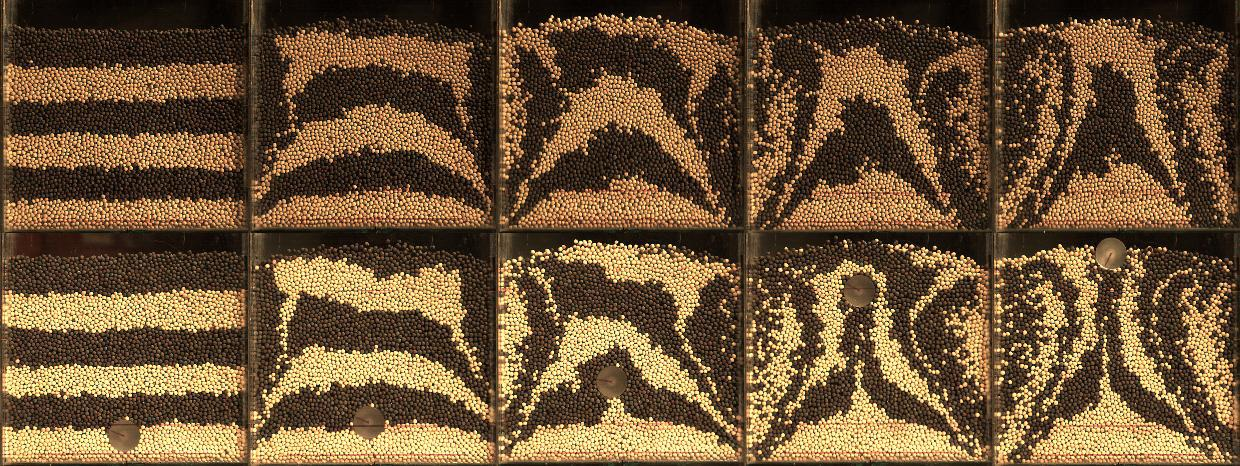
\includegraphics[width=0.65\textwidth]{04-figuras/BNE_Hejmady_Convection.png}
    \caption[Granular convection in vibrated bed.]{Evolution of the vibrated bed. Top Panels are without intruder, while bottom Panels are with an intruder. Black and yellow layers are made of mustard grains. Figure taken from \cite{Scaling_behavior_in_convection-driven_Brazil-nut_effect}.}
    \label{fig:BNE_hejmady_convection}
\end{figure}

    One of the firsts attempts to explain the BNE was made by Rosato \textit{et al.} \cite{Why_the_Brazil_nuts_are_on_top} using Monte Carlo simulations and inspired many works to classify the roles of the parameters. As an example of the larger grain rising with respect to time, Figure \ref{fig:BNE_rosato}.

\begin{figure}
    \centering
    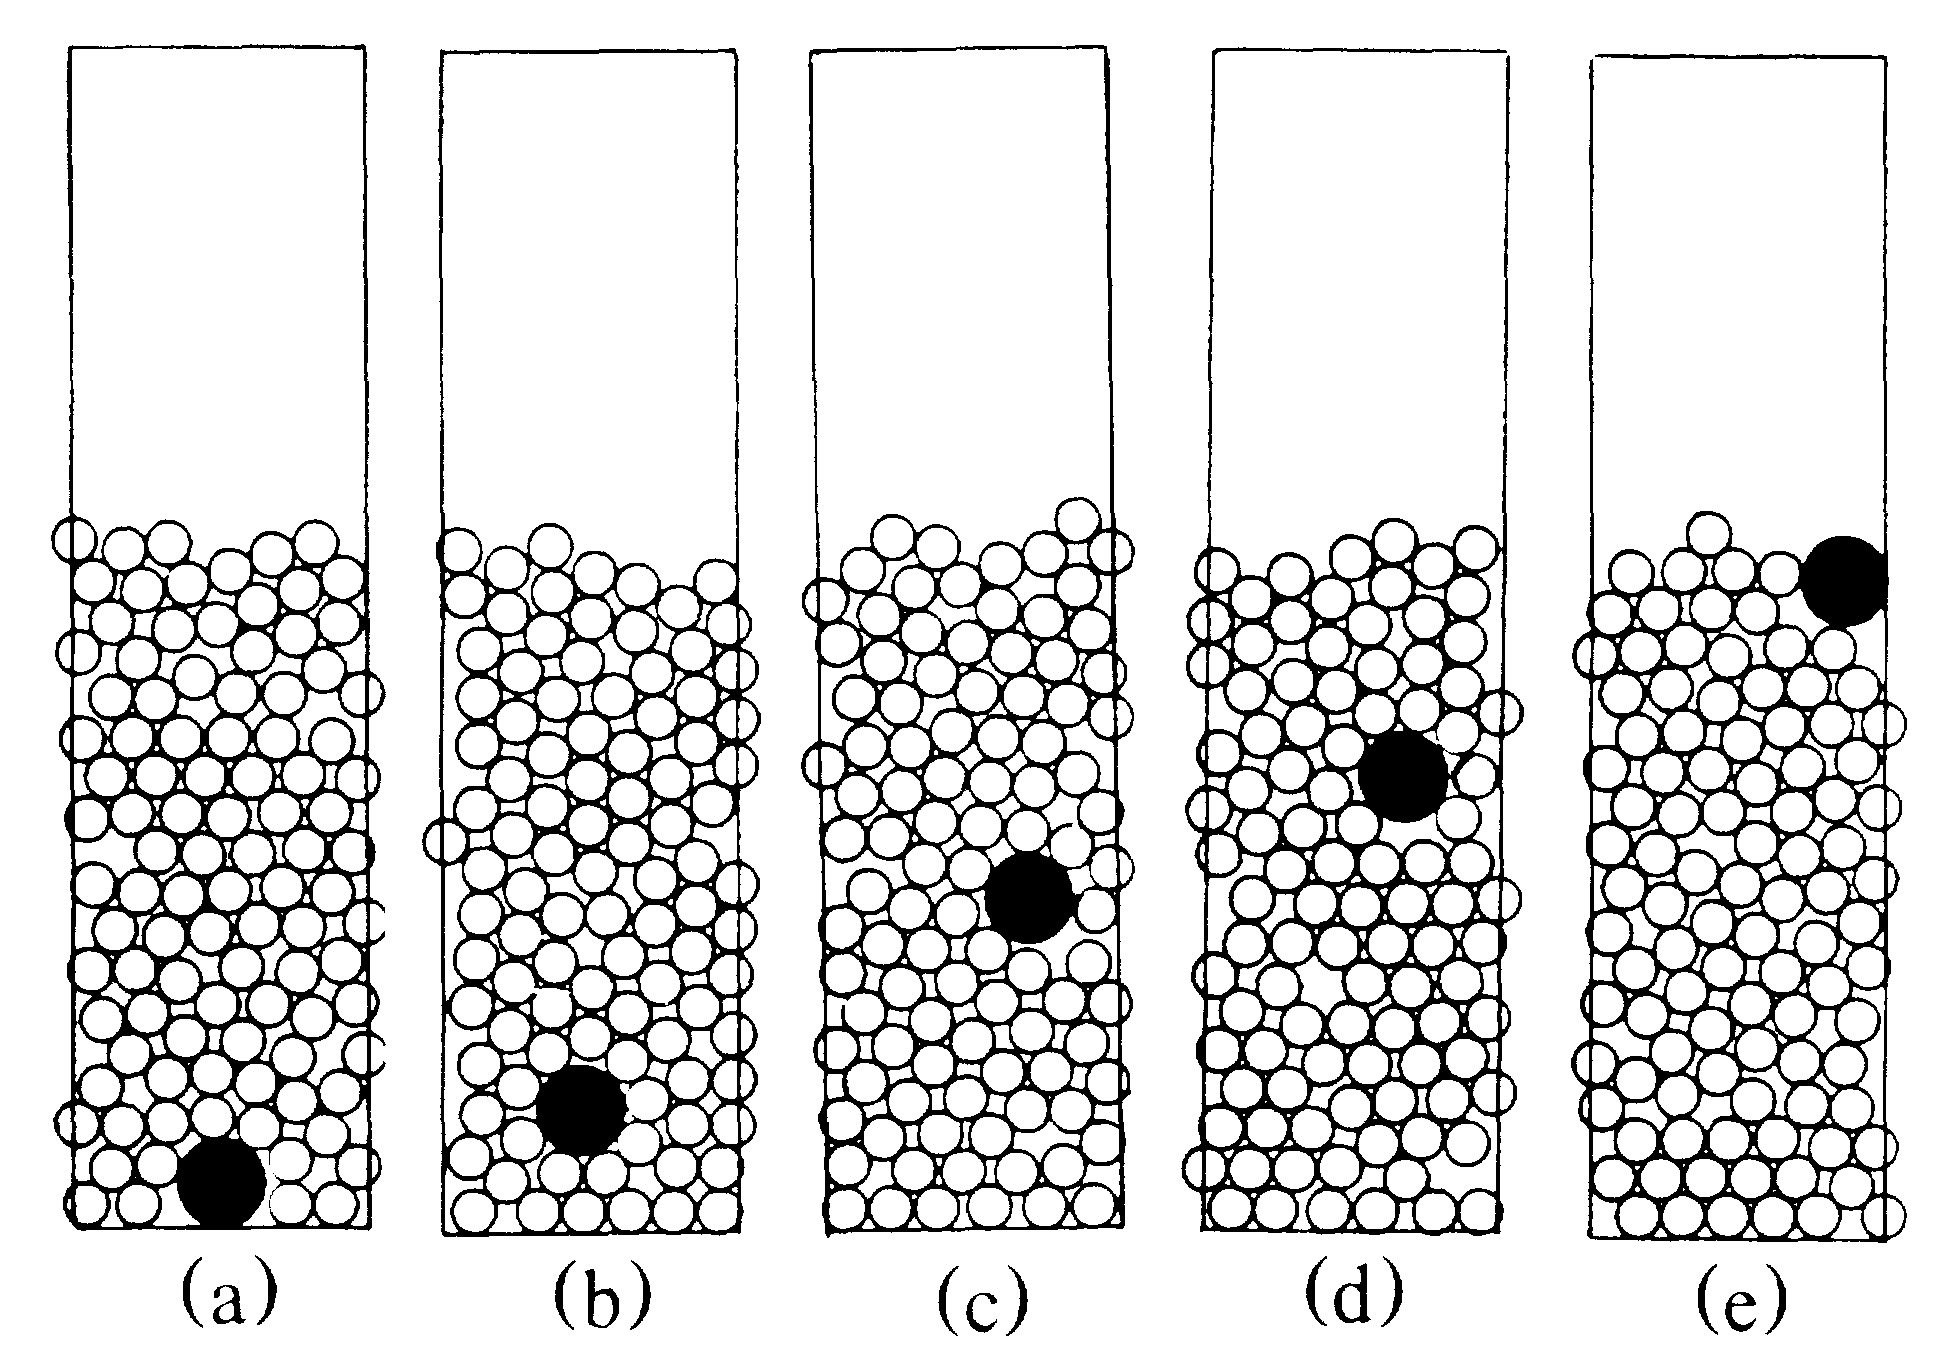
\includegraphics[width=0.65\textwidth]{04-figuras/BNE_Rosato.png}
    \caption[BNE cycles.]{Temporal evolution of shaken system of particles with periodic boundary conditions using Monte Carlo simulation. Initial configuration in Panel (a) and equally time spaced from Panels (a) to (e). Figure taken from \cite{Why_the_Brazil_nuts_are_on_top}.}
    \label{fig:BNE_rosato}
\end{figure}

%    Vários diagramas de fase foram observados para alguns dos parâmetros do BNE. Dentre as principais variáveis estão a razão de diâmetros dos grãos e a razão de densidades \cite{A_Horizontal_Brazil-Nut_Effect_and_Its_Reverse, Brazil-Nut_effect_Size_separation_of_granular_particles, Brazil-nut_effect_versus_reverse_Brazil-nut_effect_in_a_moderately_dense_granular_fluid, Categorization_of_Brazil_nut_and_its_reverse_under_less-convective_conditions_for_microgravity_geology, Competition_of_Brazil_nut_effect_buoyancy_and_inelasticity_induced_segregation_in_a_granular_mixture, Reverse_Brazil_Nut_Problem_Competition_between_Percolation_and_Condensation, Reversing_the_Brazil-Nut_Effect_Competition_between_Percolation_and_Condensation, Reverse_buoyancy_in_a_vibrated_granular_bed_Computer_Simulations, Scaling_behavior_in_convection-driven_Brazil-nut_effect, Segregation_in_a_fluidized_binary_granular_mixture_Competition_between_buoyancy_and_geometric_forces, Simple_model_for_reverse_buoyancy_in_a_vibrated_granular_system}. Dentro das caracterizações dos planos de fase, a aceleração adimensional, mostrado na equação \ref{equ:gamma}, é o parâmetro de comparação relacionado à subida do intruso.
    The most important number used in the BNE studies is the dimensionless acceleration, shown in the equation \ref{equ:gamma}. The dimensionless number is a comparison between the maximum amplitude of the vibrational acceleration and gravity. 
\begin{equation}
    \label{equ:gamma}
    \Gamma = \frac{A\omega^{2}}{g},
\end{equation}
%em que $\Gamma$ é o adimensional, $A$ é a amplitude de vibração do sistema, $\omega$ é a frequência de vibração e $g$ é o valor da gravidade.
where $\Gamma$ a dimensionless number that compares shaken acceleration with gravity, $A$ is the system amplitude of the vibration, $\omega$ is the frequency of vibration, and $g$ is the value of gravity. When $\Gamma > $ 1, then the intruder can rise, since the ascending part of the oscillation rises the magnitude of the chain forces in the media, but when the system is descending the lighter grains occupies the void space left by the bead, causing the ratchet effect. If $\Gamma < $ 1, then the intruder is not able to move, since chain forces stays there. This is the basic explanation, but not all cases work like it, as we see in some of our simulations, in Chapter \ref{chap:Resultados-BNE}.

    An experimental problem is proposed in \cite{Inertia_in_the_Brazil_nut_problem}, like we study in Chapter \ref{chap:Resultados-BNE}. In their experiment a metallic bead is placed at bottom and then agitated. They use a cylinder silo and spherical grains with size ratio between intruder and media of 3, and $\Gamma$ varies from 2.6 to 3.4, which leads the bead to rise over the media. There is a collapse of the curves involving the intruder position, the amplitude of the vibration $A$ and the oscillation period $\omega$ like in figure \ref{fig:BNE_molinari}. What we could find in our simulations is that frictionless walls also cause the bead to rise through convection currents, and the ascent ratio is similar with and without friction on the walls, see Figure \ref{fig:BNE25000_sem_Atrito_Parede}. %Refutar a tese de sem atrito nas paredes o sistema não funcionar. %Também refutar a ideia de que a ascenção do intruso não está correlacionada com as correntes de convecção. 

\begin{figure}
    \centering
    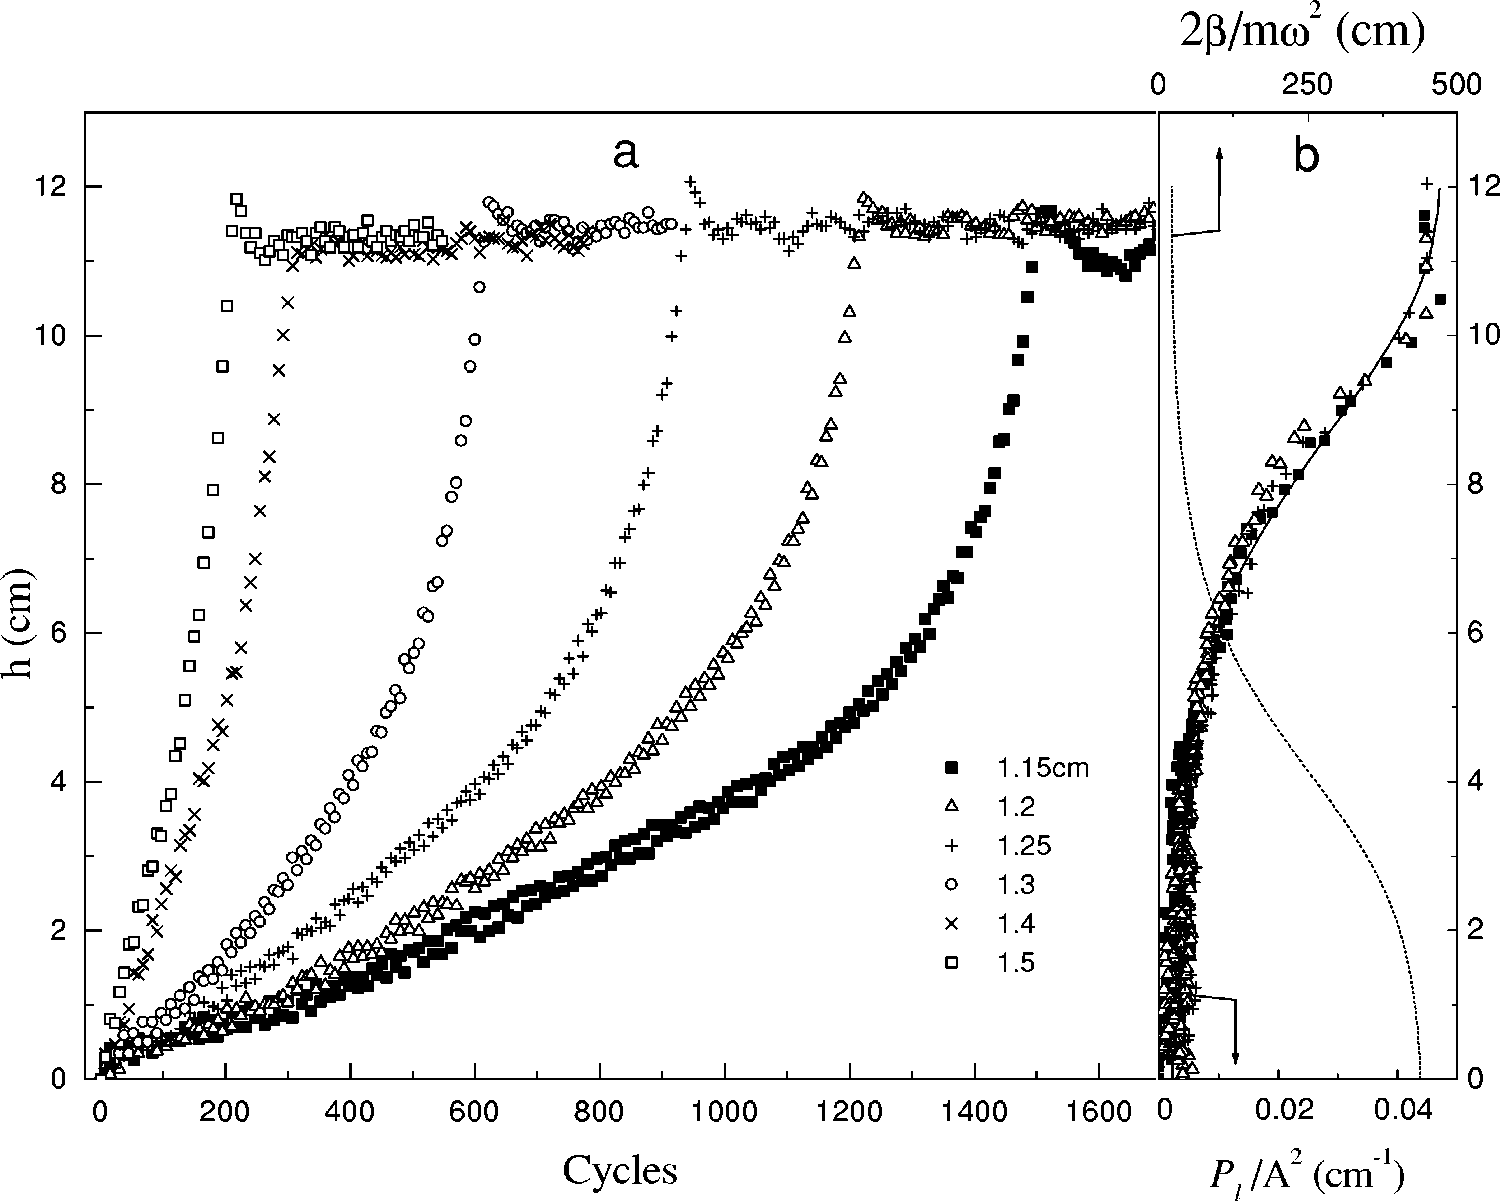
\includegraphics[width=0.65\textwidth]{04-figuras/BNE_Molinari.png}
    \caption[Intruder height in an agitated media.]{Evolution of the bead in an agitated media within a cylinder silo. Panel (a) shows the height of the intruder versus time, while Panel (b) shows the collapse of the curves. Figure taken from \cite{Inertia_in_the_Brazil_nut_problem}.}
    \label{fig:BNE_molinari}
\end{figure}

    The BNE is also influenced by the fluid that surrounds the media. In some cases, the air is relevant in the convection currents, and then leading to segregation, while vacuum leads to mixing \cite{Brazil-Nut_effect_Size_separation_of_granular_particles, Inertia_in_the_Brazil_nut_problem}. A more viscous fluid than air, like water, changes the regime of ascension of the bead, and the main mechanism that explains it is not the drag it self but the enhance of the ratcheting effect \cite{The_water-enhance_Brazil_nut_effect}.

    Several phase diagrams were observed for some of the BNE parameters. The two main variables usually analysed are the ratio of the diameters of grains and the ratio of densities of grains, as shown in Figure \ref{fig:BNE_mobius}. Another BNE phase diagram proposed by \cite{Scaling_behavior_in_convection-driven_Brazil-nut_effect} takes into account the dimensionless acceleration $\Gamma$ and the vibration threshold velocity $v_c = A \omega$.

\begin{figure}
    \centering
    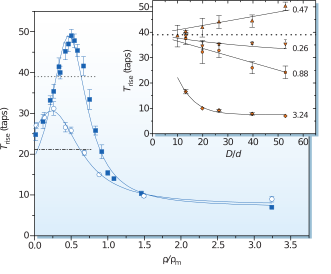
\includegraphics[width=0.65\textwidth]{04-figuras/BNE_Mobius.png}
    \caption[Phase diagram of BNE: density ratio and size ratio.]{BNE dependence on density and size ratio. The ascent time $T_{rise}$ in the main Panel versus density rate, with size ratio of 5.08 between intruder and grains with different atmospheric pressures: 1 atm. in squares ($\textcolor{blue}{\blacksquare}$) and 90 torr in circles ($\textcolor{blue}{\circ}$). The ascent time $T_{rise}$ versus the size ratio for different density ratios: 0.44, 0.48, 0.88 and 3.1. Figure taken from \cite{Brazil-Nut_effect_Size_separation_of_granular_particles}.}
    \label{fig:BNE_mobius}
\end{figure}

\begin{figure}
    \centering
    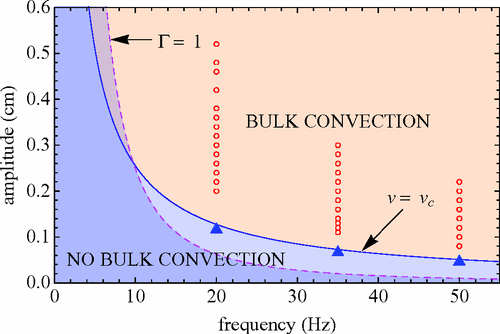
\includegraphics[width=0.65\textwidth]{04-figuras/BNE_Hejmady_PhaseSpace.png}
    \caption[Phase diagram of BNE: $\Gamma$ and $v_c$.]{BNE dependence on the dimensionless acceleration $\Gamma$ and a critical velocity $v_c$. Values of $\Gamma$ < 1 makes the intruder not rise, but also a $v < A \omega$. Figure taken from \cite{Scaling_behavior_in_convection-driven_Brazil-nut_effect}.}
    \label{fig:BNE_hejmady_convection}
\end{figure}

    Another correlated phenomena to BNE is the Reverse BNE (RBNE), in which the bead instead of rises it sinks. Many works enhanced the characterization of BNE and RBNE, in theoretical field, experimental results and numerical simulations \cite{A_Horizontal_Brazil-Nut_Effect_and_Its_Reverse, Brazil-nut_effect_versus_reverse_Brazil-nut_effect_in_a_moderately_dense_granular_fluid, Categorization_of_Brazil_nut_and_its_reverse_under_less-convective_conditions_for_microgravity_geology, Competition_of_Brazil_nut_effect_buoyancy_and_inelasticity_induced_segregation_in_a_granular_mixture, Reverse_Brazil_Nut_Problem_Competition_between_Percolation_and_Condensation, Reverse_buoyancy_in_a_vibrated_granular_bed_Computer_Simulations, Reversing_the_Brazil-Nut_Effect_Competition_between_Percolation_and_Condensation, Segregation_in_a_fluidized_binary_granular_mixture_Competition_between_buoyancy_and_geometric_forces, Simple_model_for_reverse_buoyancy_in_a_vibrated_granular_system, Hydrodynamic_theory_for_reverse_brazil_nut_segregation_and_the_non-monotonic_ascension_dynamics}. Some of these diagrams are presented here in Figures \ref{fig:RBNE_breu}, \ref{fig:RBNE_schnautz} and \ref{fig:RBNE_trujillo}.

\begin{figure}
    \centering
    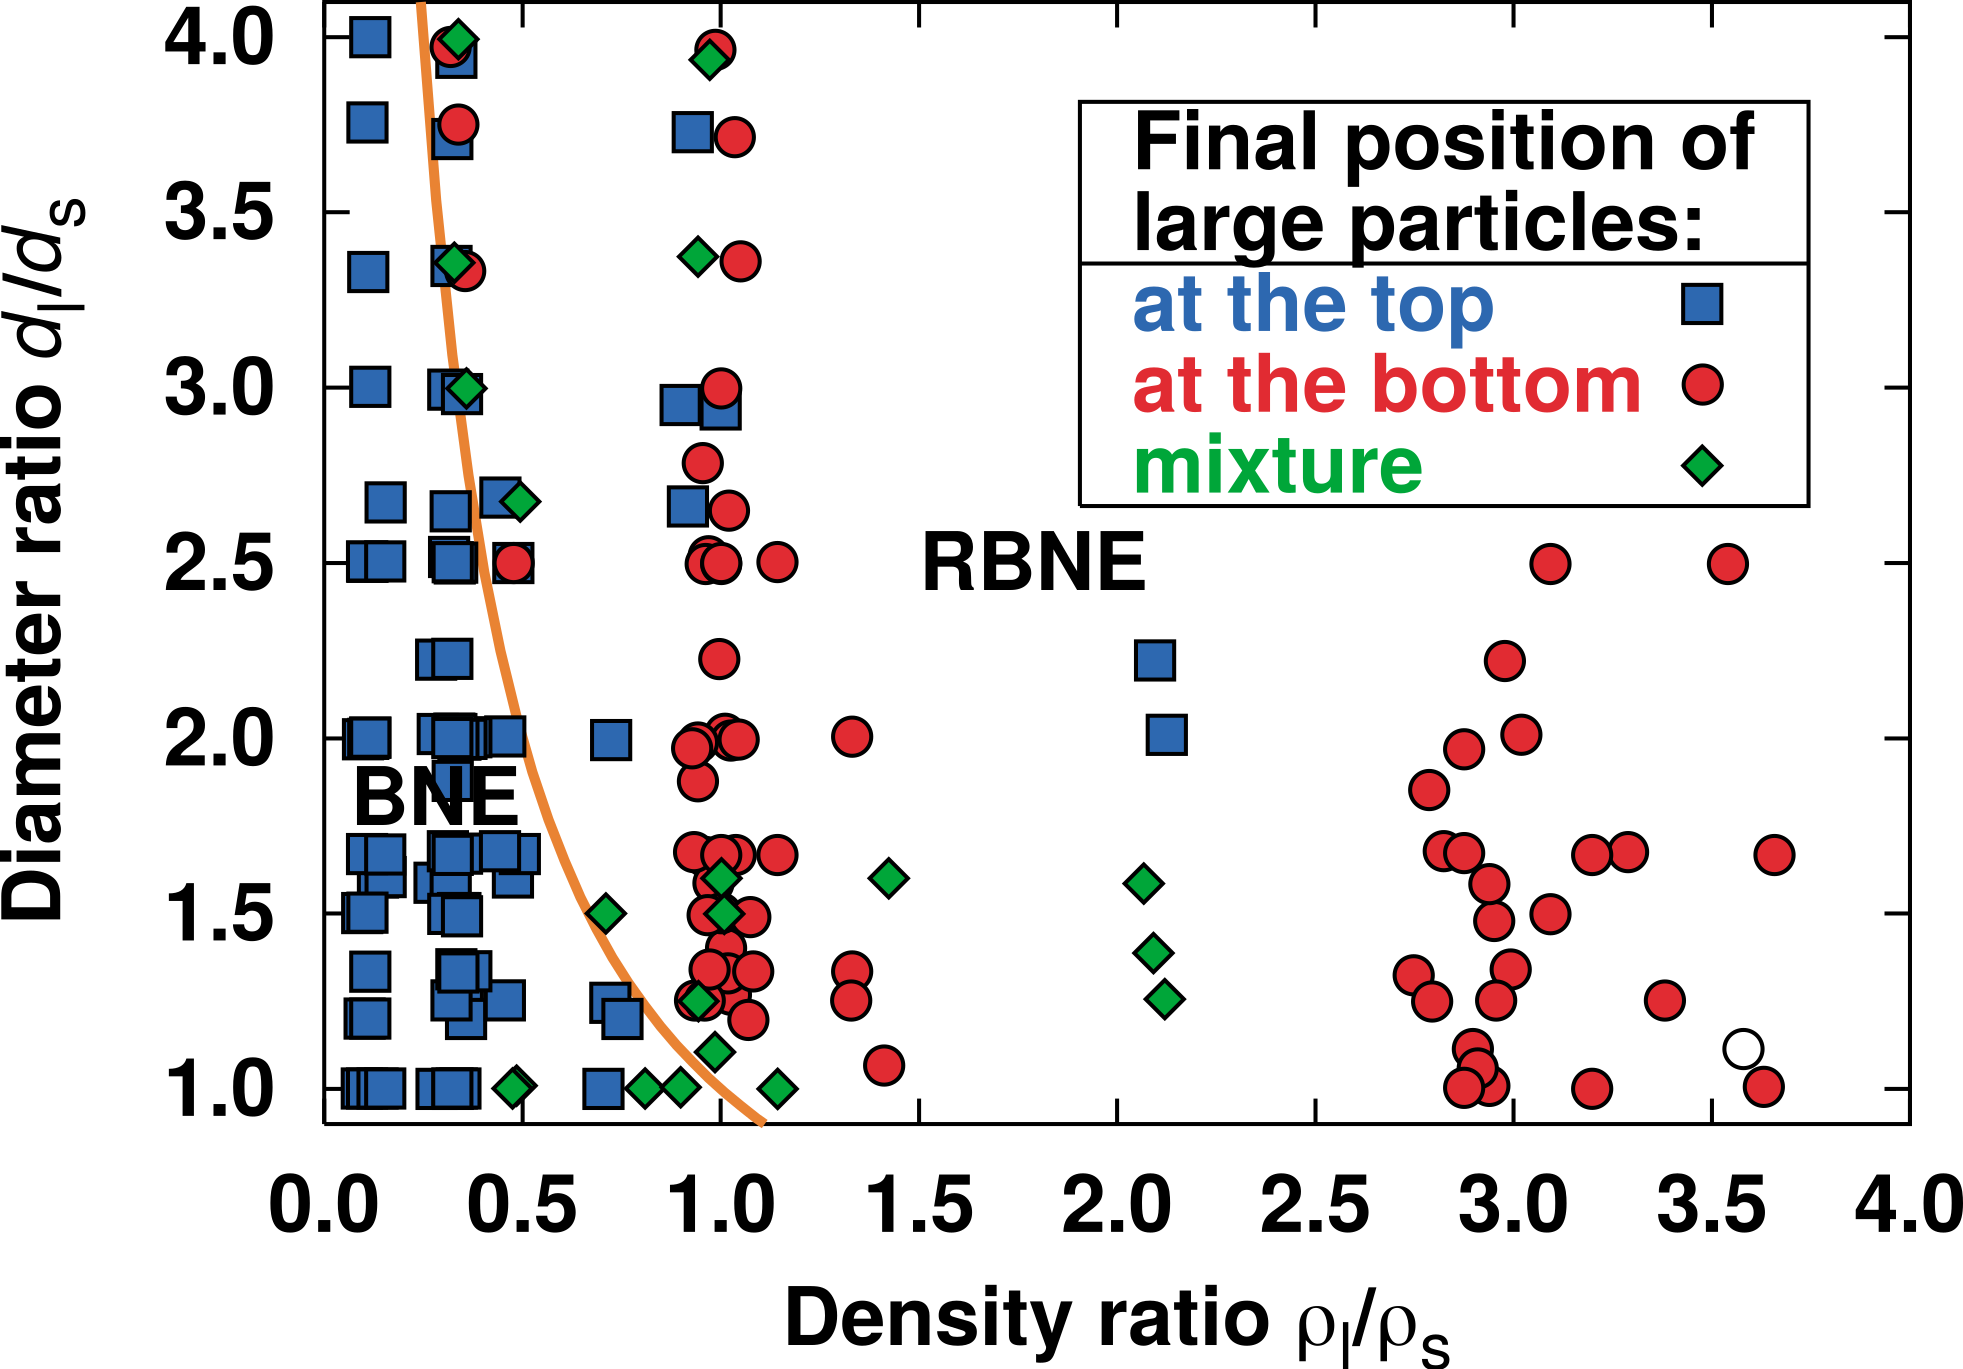
\includegraphics[width=0.65\textwidth]{04-figuras/BNE_Breu.png}
    \caption[Phase diagram of BNE/RBNE from experiment: density ratio and size ratio.]{BNE and RBNE dependence on the density ratio and the size ratio in vibrated base. The diagram shows the regime where beads rises in blue ($\textcolor{blue}{\blacksquare}$) causing the BNE, sinks in red ($\textcolor{red}{\blacksquare}$) and is mixed in green ($\textcolor{green}{\blacksquare}$). Figure taken from \cite{Reversing_the_Brazil-Nut_Effect_Competition_between_Percolation_and_Condensation}.}
    \label{fig:RBNE_breu}
\end{figure}

\begin{figure}
    \centering
    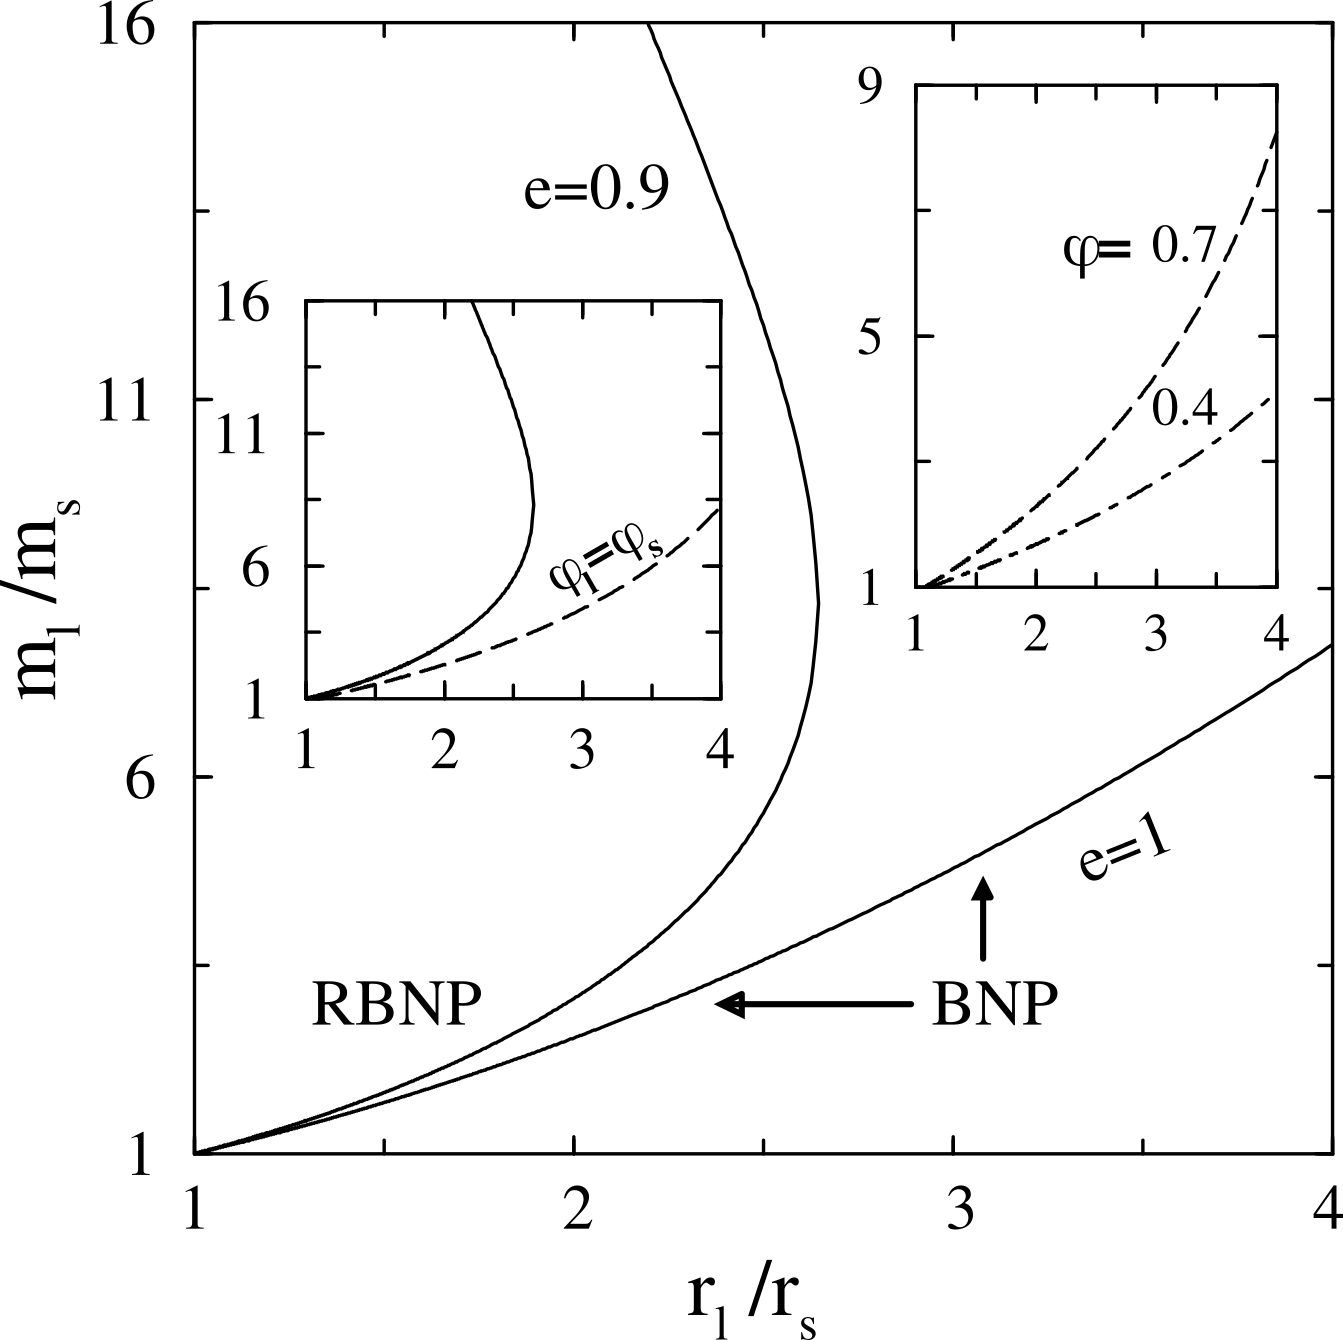
\includegraphics[width=0.65\textwidth]{04-figuras/BNE_Trujillo.png}
    \caption[Phase diagram of BNE/RBNE from analytics: density ratio and size ratio.]{BNE and RBNE dependence on the density ratio and the size ratio in vibrated base. The diagram shows the BNE-RBNE regime extracted from analytical equations of the forces in the system. $e$ is the restitution coefficient, $\phi$ is the packing fraction, $\phi_{l}$ is the portion of the packing fraction related to the intruders, $\phi_{s}$ is the packing fraction of the other grains. Left inset: phase diagram with $e$ = 0.9, $\phi_{l} / \phi_{s}$ = 10$^{-8}$ (solid curve) and $\phi_{l} / \phi_{s}$ = 1 (dashed curve). Right inset: phase diagram with $e$ = 0.9, $\phi_{l} / \phi_{s}$ = 1, $\phi$ = 0.7 (dashed curve) and $\phi$ = 0.4 (dot-dashed curve). Figure taken from \cite{Segregation_in_a_fluidized_binary_granular_mixture_Competition_between_buoyancy_and_geometric_forces}.}
    \label{fig:RBNE_trujillo}
\end{figure}

\begin{figure}
    \centering
    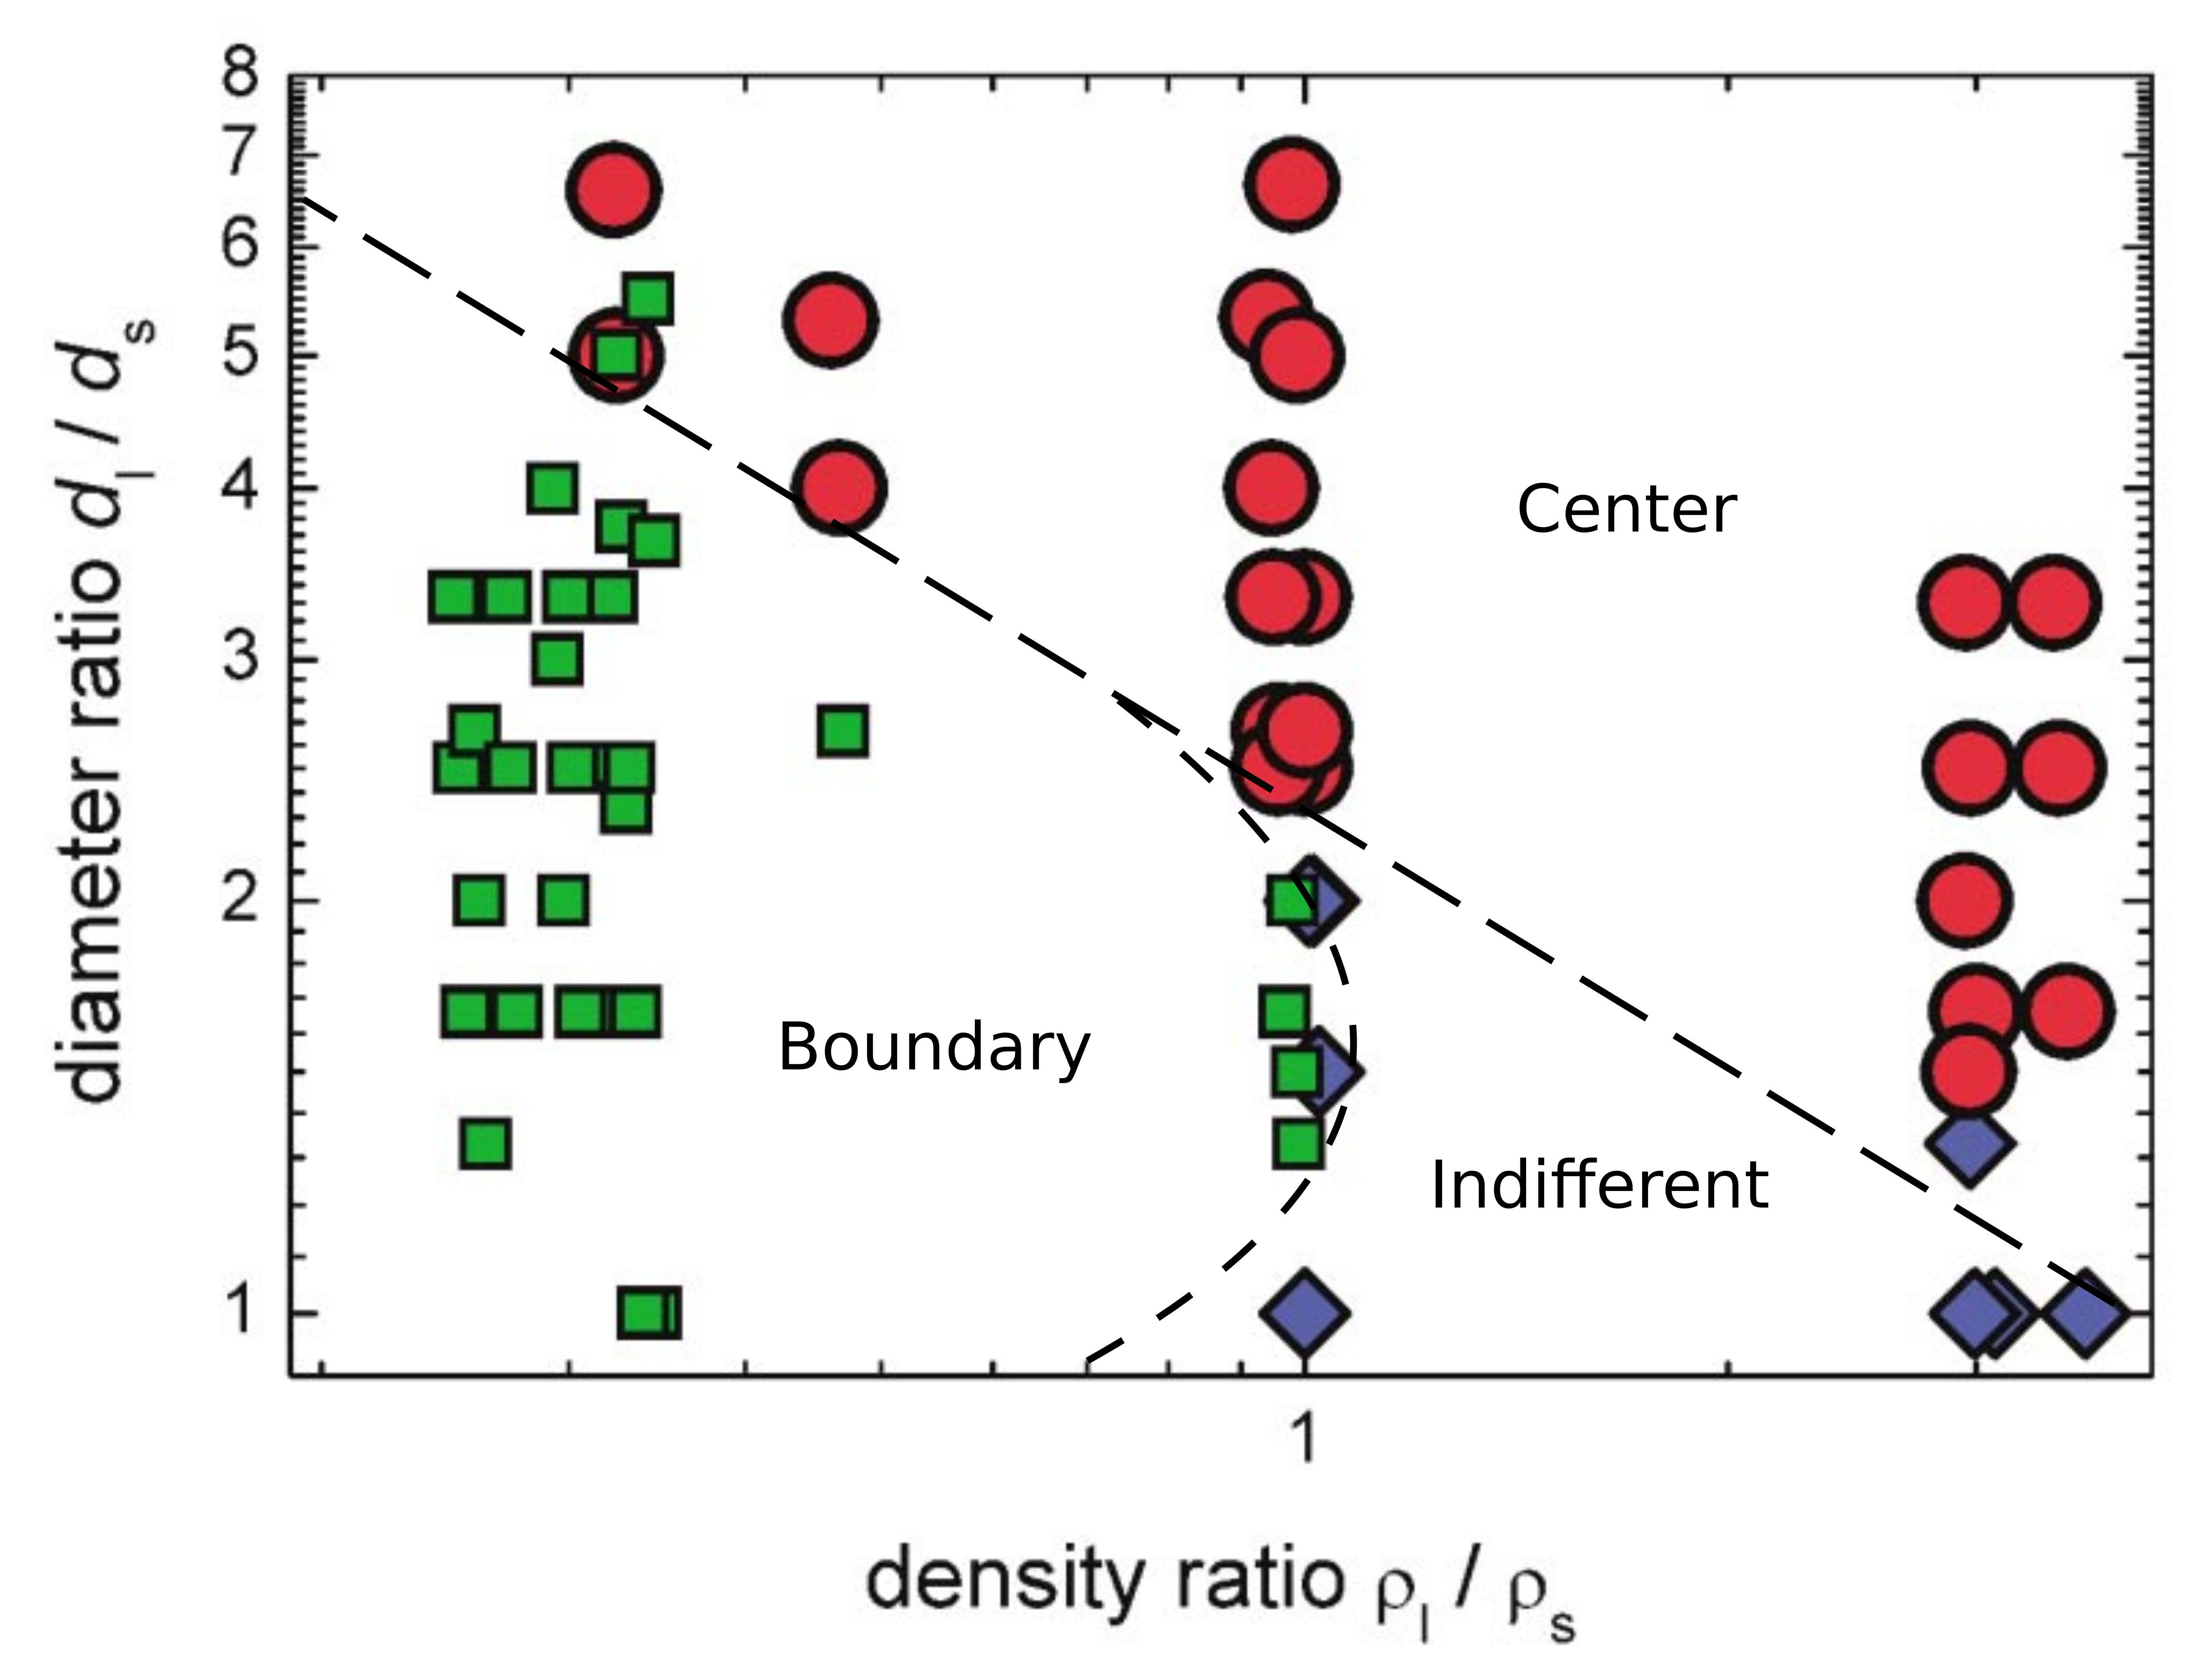
\includegraphics[width=0.65\textwidth]{04-figuras/BNE_Schnautz.png}
    \caption[Phase diagram of BNE/RBNE in swirling: density ratio and size ratio.]{BNE and RBNE dependence on the density ratio and the size ratio in swirling base. The diagram shows the regime where beads segregates in red ($\textcolor{red}{\CIRCLE}$), aggregates in green ($\textcolor{green}{\blacksquare}$) and is indifferent in blue ($\textcolor{blue}{\Diamondblack}$). Figure taken from \cite{A_Horizontal_Brazil-Nut_Effect_and_Its_Reverse}.}
    \label{fig:RBNE_schnautz}
\end{figure}

    Recently the Reference \cite{Size_segregation_of_irregular_granular_materials_captured_by_time-resolved_3D_imaging} experimentally shows that in a mixture of irregular ellipsoidal shape firstly reorient vertically, but without changing significantly their height; secondly, the grains rise upwards, and while doing so, they still tend to stay vertically aligned; and finally, when the grains reach the top, they tend to realign horizontally on the surface.

    If the intruder of the media has a non uniform distribution geometry, like a polar particle, inserted in a layer of circular grains, and when the media is agitated, the intruder starts to "self-propel" at the direction it is oriented \cite{Symmetry_properties_of_the_large-deviation_function_of_the_velocity_of_a_self-propelled_polar_particle}. This is another property that non uniform shaken granular exhibit, reorienting the position or "propelling-itself".

    %Referência do intruso andando no meio granular (está no artigo e inspirou o uso do LDF).

%Reverse BNE: A_Horizontal_Brazil-Nut_Effect_and_Its_Reverse, Brazil-nut_effect_versus_reverse_Brazil-nut_effect_in_a_moderately_dense_granular_fluid, Caracterization_of_Brazil_nut_and_its_reverse_under_less-convective_conditions_for_microgravity_geology, Competition_of_Brazil_nut_effect_buoyancy_and_inelasticity_induced_segregation_in_a_granular_mixture, Reverse_Brazil_Nut_Problem_Competition_between_Percolation_and_Condensation, Reverse_buoyancy_in_a_vibrated_granular_bed_Computer_Simulations, Reversing_the_Brazil-Nut_Effect_Competition_between_Percolation_and_Condensation, Segregation_in_a_fluidized_binary_granular_mixture_Competition_between_buoyancy_and_geometric_forces, Simple_model_for_reverse_buoyancy_in_a_vibrated_granular_system, Hydrodynamic theory for reverse brazil nut segregation and the non-monotonic ascension dynamics
%Vibrações verticais: Inertia_in_the_Brazil_nut_problem, The_water-enhance_Brazil_nut_effect, Brazil-Nut_effect_Size_separation_of_granular_particles, Caracterization_of_Brazil_nut_and_its_reverse_under_less-convective_conditions_for_microgravity_geology, Competition_of_Brazil_nut_effect_buoyancy_and_inelasticity_induced_segregation_in_a_granular_mixture, Reverse_buoyancy_in_a_vibrated_granular_bed_Computer_Simulations, Reversing_the_Brazil-Nut_Effect_Competition_between_Percolation_and_Condensation, Scaling_behavior_in_convection-driven_Brazil-nut_effect
%Vibrações laterais: Size_segregation_of_irregular_granular_materials_captured_by_time-resolved_3D_imaging, A_Horizontal_Brazil-Nut_Effect_and_Its_Reverse, 

%    No próximo capítulo, descreveremos os resultados obtidos ao simularmos o BNE.
    Next Chapter, we describe the results of our BNE simulations using the techniques presented in Chapter \ref{chap:DEM}.

%    Inertia_in_the_Brazil_nut_problem -> Atribui a convecção ao atrito das paredes e colapsa as curvas de ascensão.
%    The_water-enhance_Brazil_nut_effect -> Uso do fluido intersticial com BNE.
%    Why_the_Brazil_Nuts_are_on_top -> Atribui o BNE ao efeito catraca, usando Monte Carlo e desprezando atrito e a massa é desprezível para o efeito.
%    A_Horizontal_Brazil-Nut_Effect_and_Its_Reverse -> Vibra horizontalmente e com diferentes materiais (densidades), reproduz BNE (ida para o centro) e rBNE (ida para as bordas). Frequências de 0.5 à 2Hz, amplitude de $3,175n$mm, com $n$ variando de $3 ... 7$, diâmetro médio dos grãos de 6mm, diâmetro do intruso $1,3 ... 7$ vezes o diâmetro dos grãos e coeficiente de atrito de $0,67$. Exibe um diagrama de fase Diâmetro/Densidade.
%    Brazil-Nut_effect_Size_separation_of_granular_particles -> Descreve o fenômeno em função do diâmetro e da densidade, fixa a frequência em $13$Hz e a amplitude em $7,35$mm e o diâmetro do grão menor em $0,5$mm, ou seja, a relação amplitude e diâmetro do grão é de $14,7$ vezes. Diâmetro do intruso pode chegar à $25,4$mm, o equivalente $50800$ vezes o diâmetro do grão.
%    Brazil-nut_effect_versus_reverse_Brazil-nut_effect_in_a_moderately_dense_granular_fluid -> Analítico/teórico sobre os planos de fase das regiões BNE e rBNE em função do diagrama Diâmetro/Densidade com coeficiente de compactação e restituição.
%    Caracterization_of_Brazil_nut_and_its_reverse_under_less-convective_conditions_for_microgravity_geology -> Reproduz o BNE em condição fechada, porém com atrito baixo entre parede/grão, com condições de aceleração menores q a gravidade.
%    Competition_of_Brazil_nut_effect_buoyancy_and_inelasticity_induced_segregation_in_a_granular_mixture -> Compara os resultados do BNE em função das massas, diâmetros e coeficientes de restituição.
%    Reverse_Brazil_Nut_Problem_Competition_between_Percolation_and_Condensation -> Mostra o diagrama qualitativo da transição BNE para rBNE em função da razão dos diâmetros pelas massas. Relaciona a temperatura granular.
%    Reverse_buoyancy_in_a_vibrated_granular_bed_Computer_Simulations -> Insere um fluido como amortizador e demonstra as forças e seus efeitos.
%    Reversing_the_Brazil-Nut_Effect_Competition_between_Percolation_and_Condensation -> Mostra o diagrama BNE/rBNE em função da densidade versus diâmetro, com o diagrama de frequência por aceleração normalizada.
%    Scaling_behavior_in_convection-driven_Brazil-nut_effect ->  mostra o esquema de convecção para a contribuição no BNE
%    Segregation_in_a_fluidized_binary_granular_mixture_Competition_between_buoyancy_and_geometric_forces -> Diagrama BNE/rBNE densidade versus diâmetro
%    Simple_model_for_reverse_buoyancy_in_a_vibrated_granular_system -> Velocidade no BNE/rBNE densidade
%    Study_the_effect_of_vibration_frequency_and_amplitude_on_the_quality_of_fluidization_of_a_vibrated_granular_flow_using_discrete_element_method -> Caracteriza o fluido em função da altura do sistema.

%    Size_separation_in_vibrated_granular_matter -> Compilado dos artigos acima

%    Convection_Cells_in_Vibrating_Granular_Media -> Em relação ao BNE não é mostrado, uma vez q a distribuição dos raios dos grãos são próximas entre si. Mostra a convecção na agitação dos granulares, mesmo quando possuem condição periódica de contorno. Porém a agitação é muito alta.
 % Fundamentação teórica - BNE
\chapter{Sediment transport}
\label{chap:Transporte-Sedimentos}
    The sediment transport is the movement of solid particles, carried by a fluid over a distance, flowing in the same direction. The transport is a combination of action of gravity on the system and the fluid forces, mainly the fluid drag force. A vast number of phenomena are related to the fluid transport, such as in industrial processes (when transporting ores through a pipeline), or the transformation of landscapes (in the formation or disappearance of dunes) \cite{Granular_Media_Between_Fluid_and_Solid}. The different fluids acts differently, resulting in phenomena like: pluvial erosion, river erosion and silting, all caused by water; and phenomena caused by wind, like dunes and desertification. 

    The types of transport can be classified as shown in Figure \ref{fig:transport_mode}, in which sediments are removed from one location and deposited into another, in different temporal and spatial scales. A formation can appear on the scale of minutes from a few centimetres high on the bottoms of rivers and oceans, to geological formations thousands of years old and hundreds of kilometres long.

\begin{figure}[H]
    \centering
    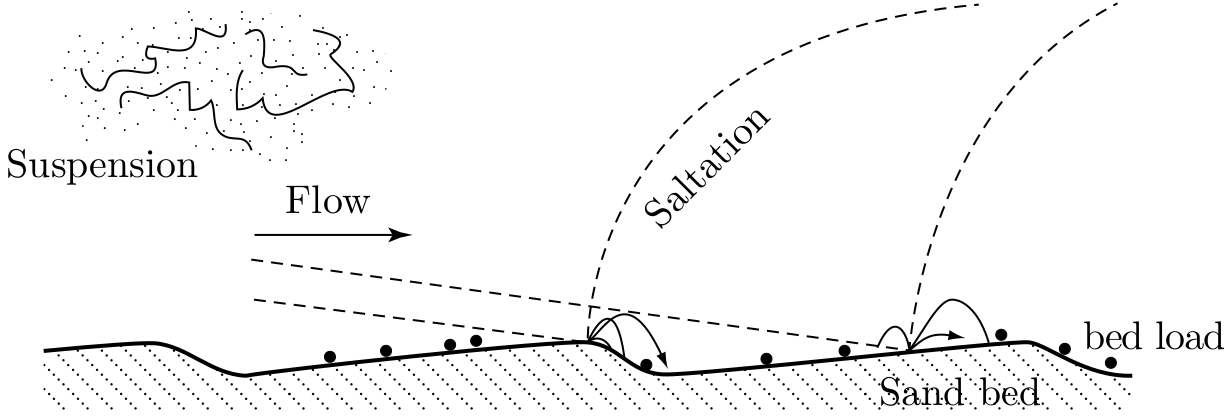
\includegraphics[width = 0.75 \textwidth]{04-figuras/TransportModes.png}
    \caption[Transport modes.]{Schematic diagram of different transport modes. Figure taken from \cite{Granular_Media_Between_Fluid_and_Solid}.}
    \label{fig:transport_mode}
\end{figure}

    Solid materials can be transported by the following modes: bedload, which is the transport of material rolling over a thin layer of the granular base and occurs when the gravitational force is the most prevalent force in the system \cite{Bedforms_in_a_turbulent_stream}. Bedload can occur on the bottom of streams and lakes and on the surface of a land. Saltation is the transport mode of materials that collides with the granular base in jumps, occurring when gravitational and drag forces are the most relevant in the system, and can be seen in rivers and in wind erosive processes. Finally suspension is the transport mode of materials in which the drag forces caused by turbulent fluctuations become the order of magnitude of the grain weight and dominate the dynamics of the system \cite{FVSCS}. Suspension may be observed in sandstorms or when sweeping house dust. 

    Single-phase models are not able to reproduce the physics involved in this problem. Models of granular materials without the presence of fluid do not exhibit the properties of transport modes such as bedload, saltation and suspension. Likewise, fluid models without sediments are not able to describe the deposition, erosion or even saturation properties. Therefore, it is necessary that the model has the two phases described, sediment and fluid. 

    Two intrinsic properties of drag are the saturation length scale $L_\textrm{sat}$ and the saturation time scale $T_\textrm{sat}$. The saturation length scale quantifies the characteristic distance for the grains to have the maximum density transported by the fluid $q_\textrm{sat}$. The saturation time scale, on the other hand, indicates the characteristic time for the transported material density to decay when the fluid velocity decreases sharply, or for the transported material density to increase when the fluid velocity increases sharply \cite{Granular_Media_Between_Fluid_and_Solid}. The main transport governing equation is the Transport Equation, which relates the quantities:
\begin{equation}
    T_\textrm{sat} \frac{\partial q}{\partial t} + L_\textrm{sat} \frac{\partial q}{\partial x} = q_\textrm{sat} - q,
    \label{equ:transporte}
\end{equation}
where $T_{sat}$ is the saturation time that flux takes to adjust, $L_{sat}$ is the saturation length that flux takes to adjust, $q_{sat}$ is the saturated flux, $q$ is the flux, $t$ is the time and $x$ is the direction of the flux.

    Aiming at a model capable of reproducing such characteristics, the use of DEM combined with the use of FDM simulate the behavior of grains and fluid, interacting with different approaches to continuous fluid and discrete to granular material. 

    To describe the interactive behavior between fluid and granular material, we will use computer simulations based on the work of Dr. Philippe Claudin \cite{Numerical_simulation_of_turbulent_sediment_transport, Sand_ripples_and_dunes, Direct_numerical_simulations_of_aeolian_sand_ripples}. By imposing the initial conditions of the fluid, the time needed for the new regime to reach stationary conditions is measured. The number of grains flowing through the system, in the steady state, provides the saturated volumetric flow $q_\textrm{sat}$, which serves as a parameter for comparing and measuring the saturation time and the saturation length. The process is repeated for each input parameter, thus quantifying the different transitions between modes of transport.

\begin{figure}[H]
    \centering
    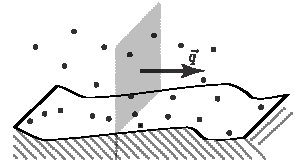
\includegraphics[width=0.65\textwidth]{04-figuras/flux_density.pdf}
    \caption[Transport volumetric flux.]{A schematic of the volumetric flux $q$. Figure taken from \cite{Granular_Media_Between_Fluid_and_Solid}.}
    \label{fig:flux_density}
\end{figure}

    The saturated flux $q_\textrm{sat}$ is the main quantity we analyze the sediment transport. It measures the volume of the particles crossing a vertical surface of unit transverse size per unit time. The definition is as it follows:
\begin{equation}
    q_\textrm{sat} = \frac{1}{A \phi_b} \frac{\pi}{6}d^3 \sum_p u^p,
    \label{equ:qsat}
\end{equation}
where $A$ is the surface area that particles cross, $\phi_b$ is the packing fraction of the base, $d$ is the average grain diameter and $u^p$ is the grain velocity.

    Other two quantities related to the saturated flux is the number of of transported grains per unit area $n$ and the mean grain horizontal velocity $u_p$:
\begin{equation}
    n = \frac{\left(\sum_p u_p\right)^2}{A\sum_p {u_p}^2}
    \label{equ:n}
\end{equation}
\begin{equation}
    \bar{u}_p = \sum_p \frac{\sum_p {u_p}^2}{\sum_p {u_p}}
    \label{equ:up}
\end{equation}
and the relation between $q_\textrm{sat}$, $n$ and $\bar{u}_p$ is:
\begin{equation}
    q_\textrm{sat} = \frac{1}{\phi_b} \frac{\pi}{6} d^3 n \bar{u}_p.
\end{equation}

\section{Threshold}
    To describe the bedload transportation threshold, we are going to write the momentum equations in steady state ($\sum F = 0$) and find the values where they get balanced, for the maximum velocity of the fluid lays the grains in rest. So, the forces that will hold grains statically until moving are given by:
\begin{equation}
    m\frac{\partial u_p}{\partial t} = F_{Drag} + F_{Friction},
\end{equation}
where the acceleration of the particle is $m\frac{\partial u_p}{\partial t} = 0$, due to the steady state regime, $F_{Drag}$ is the drag force, $F_{Friction}$ is the friction force.

\begin{equation}
    F_{Drag} = 3\pi \rho_f \nu d\left(u_f-u_p\right),
\end{equation}
is the drag force onto grains, where $\rho_f$ is the density of the fluid, $\nu$ is the viscosity of the fluid, $d$ is the diameter of the grain, $u_f$ is the fluid velocity and $u_p$ is the grains velocity.

\begin{equation}
    F_{Friction} = -\mu_s F_{Gravity},
\end{equation}
is the friction force, and is dependent of the gravity, where $\mu_s$ is the static friction coefficient, related to the Coulomb friction.

\begin{equation}
    F_{Gravity} = \frac{\pi}{6}d^3\left(\rho_p-\rho_f\right)g,
\end{equation}
is the gravity force onto the grains, where $\rho_p$ is the grains density and $g$ is the gravitational acceleration.

    And since we know that the fluid shear stress is given by:
\begin{equation}
    \tau_f = \rho_f \nu \frac{\partial u_f}{\partial z},
\end{equation}
where $\tau_f$ is the fluid shear stress, these equations combined and considering the fact that only the upper half of the particle feels drag force\footnote{As the upper layer of grains are in rest, the fluid flows more in this upper layer of grains, and almost vanish below it.}, we have:
\begin{equation}
    u_f = \frac{\tau_f}{\rho_f\nu}\frac{d}{2}.
\end{equation}
while $u_p = 0$.

    Using the Shields number (Equation \ref{equ:Shields}) and manipulating previous equations, when applied drag force is equals to friction force, we can find the threshold by:
\begin{equation}
    \Theta_t = \frac{2}{9}\mu_s,
\end{equation}
the $\Theta_t$ is the threshold that grains flow. Below this threshold grains do not move, while above it grains flows with the fluid.

\section{Contribution of moving grains}
    To introduce the contribution of the moving grains, we are still going to use most of the previous calculation. Still, particles have reached steady state, so $m\frac{\partial u_p}{\partial t} = 0$ is still valid. Considering that grains are moving, we have the balance force:
\begin{equation}
    0 = F_{Drag} + F_{Friction} + F_{Grains},
\end{equation}
now $F_{Grains}$ is the force due to the moving grains, where it is:
\begin{equation}
    F_{Grains} = \frac{\rho_p d^3 u_p \tau_p d^2}{d^2/\nu},
\end{equation}
where $\rho_p d^3 u_p$ is the momentum carried by moving grains, $\tau_p$ is the grains shear stress and $d^2/\nu$ is the characteristic time to this viscous contact dynamics.

    Looking to the limit just after the threshold, one can get a discontinuity on the grains velocity, and we expect for this behaviour an abrupt change on the friction coefficient, once we change from static regime to moving regime. Then we rewrite equations to include this term:
\begin{equation}
    \frac{3}{2}\pi\rho_f\nu d u_p = \frac{3}{2}\pi\rho_f\nu d u_f - \mu_d \frac{\pi}{6}d^3 \left(\rho_p-\rho_f\right)g,
\end{equation}
where $\mu_d$ is the new friction coefficient. Then, rewriting $u_p = v_0$ just in the limit after the threshold, we have:
\begin{equation}
    v_0 = \frac{2}{9}\left(\mu_s-\mu_d\right)v_b,
\end{equation}
where $v_b = \sqrt{\left(\frac{\rho_p}{\rho_f}-1\right)gd}$ is the normalised velocity by the grains parameters.

    Now, the grains shear stress is:
\begin{equation}
    \tau_p \propto n,
\end{equation}
where $n$ is the number of moving grains by the cross section parallel to the fluid flow divided by the area of this cross section. From previous analysis, we quantify $n$, $\overline{u}_p$ and $q$ as following:
\begin{subequations}
    \begin{empheq}{align}
        n = a_n \left( \Theta - \Theta_t \right) \frac{1}{d^2},\\
        \overline{u}_p = \mathcal{G} \, \frac{\Theta - \Theta_t + u_0}{1 - a_u \left( \Theta - \Theta_t \right)} \, u_b,\\
        q_\textrm{sat} = \frac{1}{\phi_b} \frac{\pi}{6} d^3 n \overline{u}_p,
    \end{empheq}
    \label{equ:flux_steadystate_model}
\end{subequations}
where $n$ is the number of transported grains per unit area, $a_n$ is the adjusted parameter to the data present in Figure \ref{fig:TM_profiles}(d), $\Theta$ is the Shields number, $\Theta_t$ is the threshold where transportation happens, $d$ is the average grain diameter, $\overline{u}^p$ is the mean grain horizontal velocity, $\mathcal{G}$ is the Galileo number, $u_0$ is the adjusted velocity to the data present in Figure \ref{fig:TM_profiles}(d), $a_u$ is the adjusted parameter to the data present in Figure \ref{fig:TM_profiles}(d), $u_b = \sqrt{\mathcal{D}_{R}gd}$ is the normalized velocity by the grains parameters, $q$ is the the volume of the particles (at the bed density) crossing a vertical surface of unit transverse size per unit time.
 % Fundamentação teórica - Fluido
% -----------------------------------------------------------------------------
% Resultados
% -----------------------------------------------------------------------------

\chapter{Análise e Discussão dos Resultados}
\label{chap:Resultados}

%Cada capítulo deve conter uma pequena introdução (tipicamente, um ou dois parágrafos), em seção não numerada, que deve deixar claro o objetivo e o que será discutido no capítulo, bem como a organização do capítulo.

%\section{Título da seção}
%\label{sec:titSecResult}

%Inserir seu texto aqui...
                % Resultados
%%---------------------------------- CAPITULO VI ------------------------------%
%\thispagestyle{empty}
\chapter{Cronograma e Plano de Estudos}
\section{Cronograma}
\label{ch:Chronogram}

    Apresentamos uma proposta de doutorado sanduíche para iniciar dos trabalhos com o prof. Dr. Philippe Claudin, do laboratório \textit{Physique et Méchanique des Milliex Hétérogènes} (PMMH) da \textit{École Superieure de Physique et Chemie Industrielles de la ville de Paris} (ESPCI) em Setembro de 2018 e retornar ao Brasil em Julho de 2019. A tabela \ref{tab:CronogramaFRA} contém a proposta das atividades do doutorado sanduíche. Pretende-se contribuir com o desenvolvimento científico através da escrita de ao menos um artigo, publicado em periódico que possua alto fator de impacto ao final desta parceria.

\setlength{\tabcolsep}{3pt}

\begin{table}[h]
    \begin{tabular}{| l|c|c|c|c|c|c|c|c|c|c|c |}
        \textbf{Atividades} & \multicolumn{11}{c}{\textbf{Mês do ano}}                                       \\
                                           & Set & Out & Nov & Dez & Jan & Fev & Mar & Abr & Mai & Jun & Jul \\
\hline        Revisão bibliográfica        &  X  &  X  &  X  &  X  &  X  &  X  &  X  &  X  &     &     &     \\
\hline        Equacionamento do modelo     &  X  &  X  &  X  &  X  &  X  &     &     &     &     &     &     \\
\hline        Escrita do código fonte      &     &  X  &  X  &  X  &  X  &  X  &  X  &  X  &  X  &     &     \\
\hline        Validação do modelo          &     &     &  X  &  X  &  X  &  X  &  X  &  X  &  X  &  X  &     \\
\hline        Escrita da tese              &     &     &  X  &  X  &  X  &  X  &  X  &  X  &  X  &  X  &  X  \\
\hline        Resultados preliminares      &     &     &  X  &  X  &     &     &     &     &     &     &     \\
\hline        Ajustes dos parâmetros       &     &     &     &     &     &  X  &  X  &  X  &     &     &     \\
\hline        Análise dos resultados finais&     &     &     &     &     &     &     &  X  &  X  &  X  &  X  \\
\hline \hline Participação em congresso    &     &     &     &     &  X  &  X  &     &     &     &     &     \\
\hline        Escrita do artigo            &     &     &     &     &     &     &     &     &     &  X  &  X  
    \end{tabular}
    \caption{Atividades programadas para a realização do doutorado sanduíche.}
    \label{tab:CronogramaFRA}
\end{table}

    Após o retorno ao Brasil, pretendemos seguir com o cronograma apresentado na tabela \ref{tab:CronogramaBRA}, que contempla o encerramento desta tese pela compilação dos resultados obtidos durante o tempo de desenvolvimento do sanduíche e anteriormente.

\begin{table}[h]
    \begin{tabular}{| l|c|c|c|c|c |}
        \textbf{Atividades} & \multicolumn{5}{c}{\textbf{Mês do ano}}    \\
                                           & Ago & Set & Out & Nov & Dez \\
\hline        Compilação dos resultados    &  X  &  X  &     &     &     \\
\hline        Escrita da tese              &  X  &  X  &  X  &     &     \\
\hline        Marcação da banca            &     &     &     &  X  &     \\
\hline \hline Defesa da tese               &     &     &     &     &  X
    \end{tabular}
    \caption{Atividades programadas para a realização após o retorno do doutorado sanduíche.}
    \label{tab:CronogramaBRA}
\end{table}

\section{Plano de estudos do doutorado sanduíche}
\label{ch:Estudos}

Faremos uma revisão da bibliografia baseada nos métodos de simulação de materiais granulares, o qual o candidato, o orientador e o coorientador já possuem experiência e publicações internacional. A adição as técnicas de simulação da mecânica dos fluidos ao problema caracteriza-o como um problema de transporte. Tal revisão tem o intuito de aprimorar as técnicas computacionais e o melhor embasamento no equacionamento da interação entre fluido e granular, além de verificar o estado da arte e as últimas tendências do problema.

Como a definição do trabalho e de validação prévia, revemos a forma de equacionar a mecânica dos fluidos. O intuito é de encontrar uma forma computacional mais estável para resolver o FEM. Estudamos o sistema descrito no artigo \textit{"Numerical simulation of turbulent sediment transport, from bed load to saltation."}, publicado na \textit{Physics of Fluids}, de autoria do Dr. Philippe Claudin, o coorientador \cite{Numerical_simulation_of_turbulent_sediment_transport}.

Aprimoraremos o código fonte, adequando das equações que regem o sistema. Validaremos o modelo baseando-se nos resultados da literatura, como os modos de transportes e suas propriedades. Utilizaremos as métricas já descritas pela geografia física e pela mecânica estatística.

Analisaremos os resultados preliminares do transporte de grãos como base para o início da validação das equações do modelo e das regras que regem o sistema, a fim de obter resultados que exprimam a realidade. Em seguida, ajustaremos os parâmetros necessários para a realização específica das propriedades na qual desejamos observar e documentar em forma de artigos e na base da tese a ser escrita.

A participação em um congresso na área e a publicação em periódico internacional de relevância tornam-se de importantes para a divulgação das ideias e dos resultados. O congresso tem objetivo de fazer contatos com outros grupos de pesquisa, aprimorando assim as habilidades e a colaboração entre os assuntos tratados em âmbito internacional. O artigo promove boa oportunidade posicionar bem o Brasil e o CEFET-MG com as revistas de relevância para a ciência internacional. O código fonte é um dos produtos diretos da pesquisa, e que pode ser patenteado após a conclusão da mesma.

                % Cronograma
% -----------------------------------------------------------------------------
% Conclusão
% -----------------------------------------------------------------------------

\chapter{Conclusions}
\label{chap:Conclusao}
    First of all, we successfully use the DEM technique to simulate dry granular materials and we coupled it with FDM to simulate the transport fluid.

%    Para os as simulações do BNE conseguimos reproduzir as propriedades de ascessão do intruso com diferentes densidades, diferentes amplitudes de vibração e diferentes frequências de vibração, observando a importância do atrito nas paredes do sistema. Mais do que isso, conseguimos realizar o BNE em um sistema que possui condição periódica de contorno e suas diferenças para o sistema de caixa fechada.
    For the BNE simulations we were able to reproduce the intruder's ascent properties with different densities, different vibration amplitudes and different vibration frequencies, noting the importance of frictional walls on convection effect of the system. More than that, we were able to perform the BNE in a system that has a periodic boundary condition and its differences to the closed box system. We characterized the intruder's ascent rate according to the shaken frequency, understanding that the BNE phenomena in this conditions can be interpreted as a resonance effect. An important metric was applied, enhancing our understanding of the BNE phenomena: the LDF.

%    Para o sedimento de transportes, conseguimos validar as propriedades físicas que regem o sistema, condizendo simulação com a conservação de movimento. Validamos o fluido de acordo com a literatura e acoplamos grão e fluido de forma a interagirem sobre as leis da física.

    For the sediment transport, we were able to validate the physical properties that govern the system, matching simulation with movement conservation. We validate the fluid according to the literature and couple grain and fluid so that they interact under the laws of physics. We also extracted and characterized the transport law for viscous bedload regime exploring systematically two parameters: the Galileo number $\mathcal{G}$ and the Shields number $\Theta$. Well characterized the steady-state, we moved to the transient regime, exploring the saturation time $T_\textrm{sat}$ and further the saturation length $L_\textrm{sat}$. We could deduce constitutive relations from force balance and from dimensionless analysis.

%Procure fazer uma análise crítica de seu trabalho, destacando os principais resultados e as contribuições deste trabalho para a área de pesquisa.

\section{Future works}
\label{sec:trabalhosFuturos}

    At this moment, we are finishing the last simulations to extract the saturation length $L_\textrm{sat}$ and preparing the manuscript documenting our results of the viscous bedload transport. We plan to submit this work on the Journal of Fluid Mechanics, detailing all the work we did until now in this subject.

    We also plan to analyse the fluctuations in the BNE when the intruder enters in the convection current in problems with fw, and we think in how to explore this problem using the metrics of the energy, relating the BNE with its loss of energy.

    Personally, I am planning to improve the numerical technique to simulate 3D granular materials, and extend the CFD also to 3D to analyse dune formations in viscous transportation. The CFD field is vast, but I wish to simulate mesh techniques using Discret Fourier Transform (DFT), since the fast algorithm, Fast Fourier Transform (FFT), is executable in the order of $\mathcal{O}(n \log{n})$ and seems to be perfectly matching with the granular phase.

%Também deve indicar, se possível e/ou conveniente, como este trabalho pode ser estendido ou aprimorado.

%\section{Considerações Finais}
%\label{sec:consideracoesFinais}

%As derradeiras palavras para encerramento do seu trabalho acadêmico.

% -----------------------------------------------------------------------------
% OBS: a norma ABNT estabelece que em qualquer tipo de trabalho acadêmico monográfico
% deve haver um capítulo de conclusão
% -----------------------------------------------------------------------------
                 % Conclusão

% Insere os elementos pós-textuais
\postextual
% -----------------------------------------------------------------------------
% Referências
% -----------------------------------------------------------------------------

% -----------------------------------------------------------------------------
% Carrega o arquivo "base-referencias.bib" e extrai automaticamente as referências citadas
% -----------------------------------------------------------------------------

\bibliography{./base-referencias}{}
\bibliographystyle{abnt-num} % Define o estilo ABNT para formatar a lista de referências

% -----------------------------------------------------------------------------
% Este arquivo não necessita de ser editado.
% -----------------------------------------------------------------------------
           % Referências
\begin{apendicesenv}
\partapendices

\chapter{Artigos publicados}
\label{chap:Artigo}
    A seguir os artigos publicados desde o início desta pesquisa. O primeiro artigo apresentado refere-se a publicação feita sobre este doutoramento, com resultados mistos das técnicas utilizadas na dissertação de mestrado \cite{Dissertacao} e este projeto de tese. O segundo e terceiro artigos apresentados referem-se a publicações feitas durante a dissertação, mas que expressam as técnicas utilizadas neste projeto de tese.

\section{\textit{Large-deviation quantification of boundary conditions on the Brazil nut effect}}
\label{appendix:BNE}
    This paper was published on the Physical Review E, and it is one of the main themes of this thesis, refering to chapter \ref{chap:BNE}.

\section{\textit{Methods of parallel computation applied on granular simulations}}

    Este artigo foi publicado no quatrienal do congresso \textit{Powders \& Grains 2017}, que é o maior congresso sobre materiais granulares, e que está em sua 8ª edição.

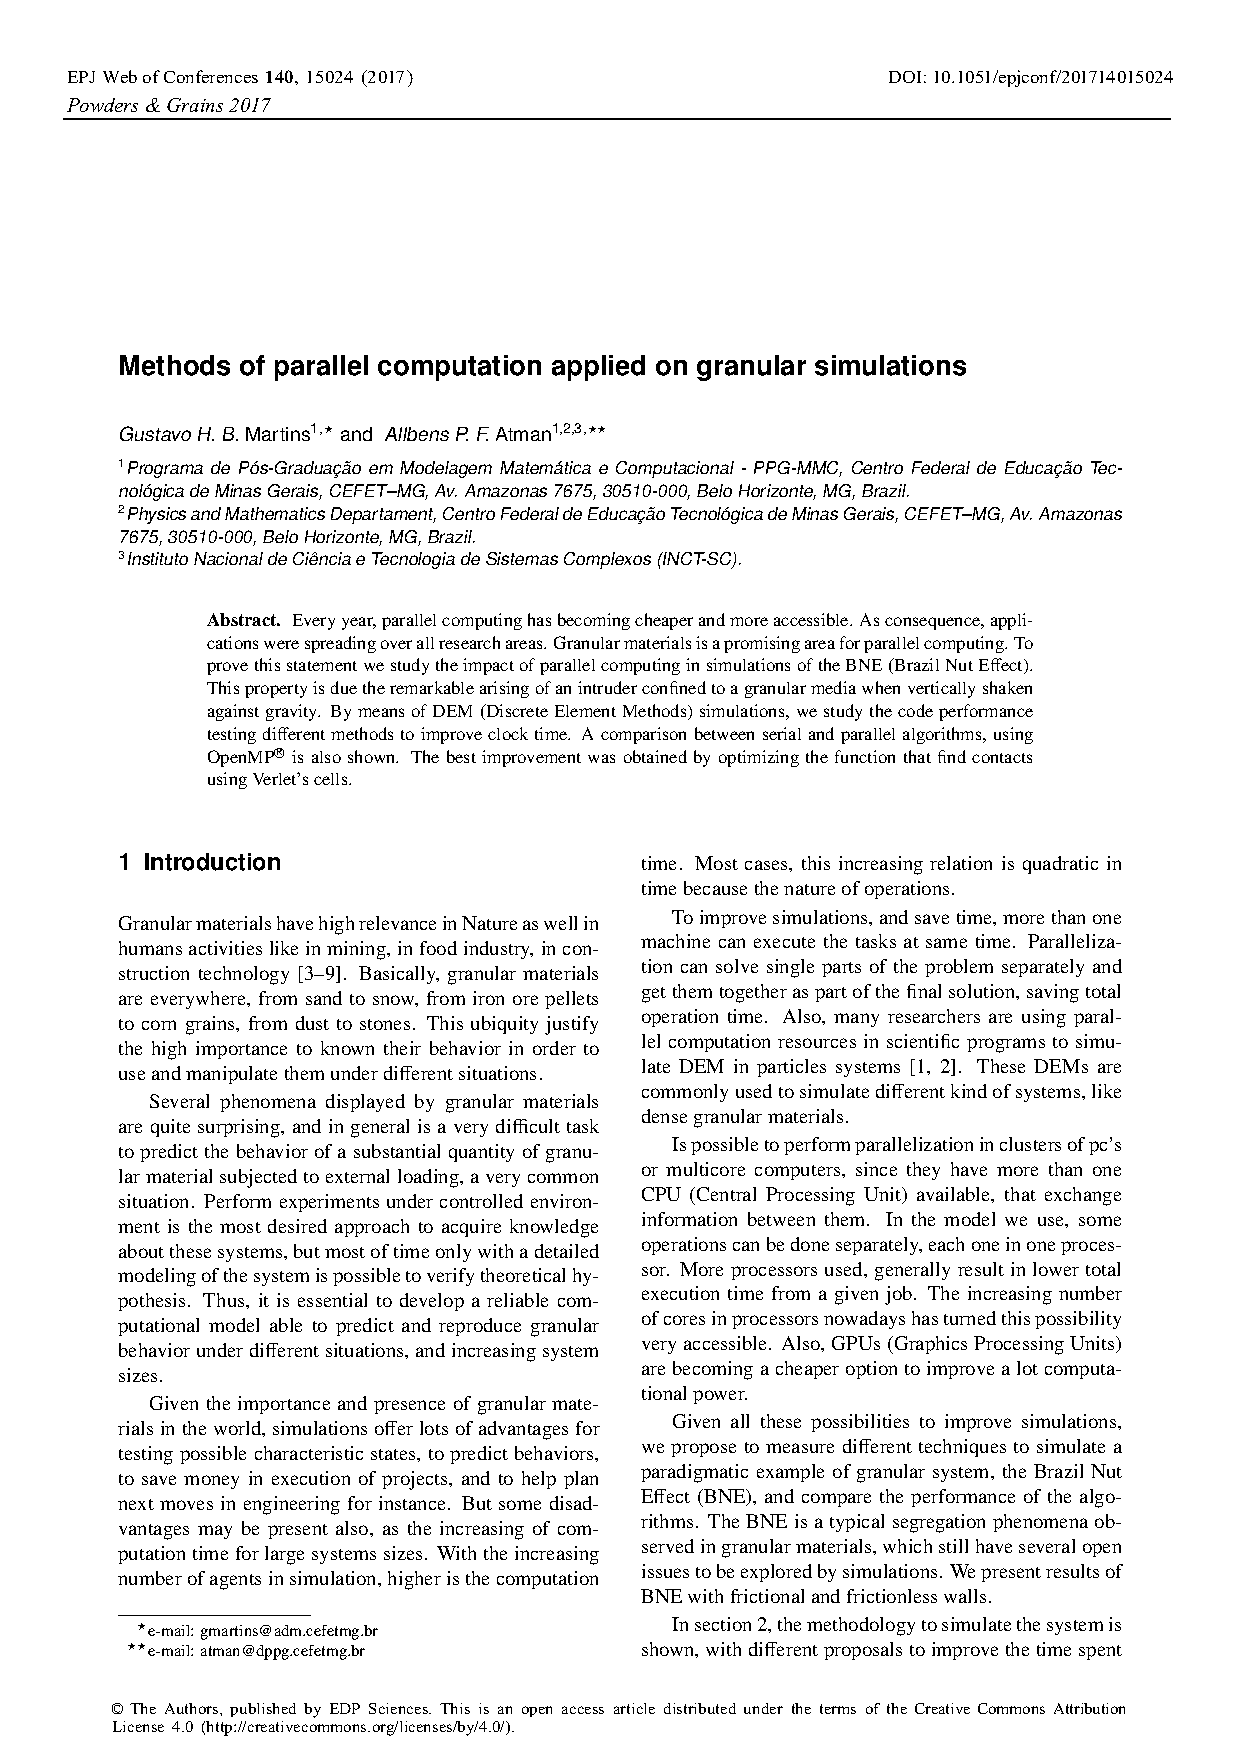
\includepdf[pages=-]{./08-apendice/ArtigoPG2017.pdf}

\section{\textit{Mechanical properties of inclined frictional granular layers}}

    Este artigo foi publicado na \textit{Granular Matter}, uma das maiores revistas sobre material granular e é uma revista A2 segundo a classificação \textit{qualis} da CAPES e possui fator de impacto de $1,762$.

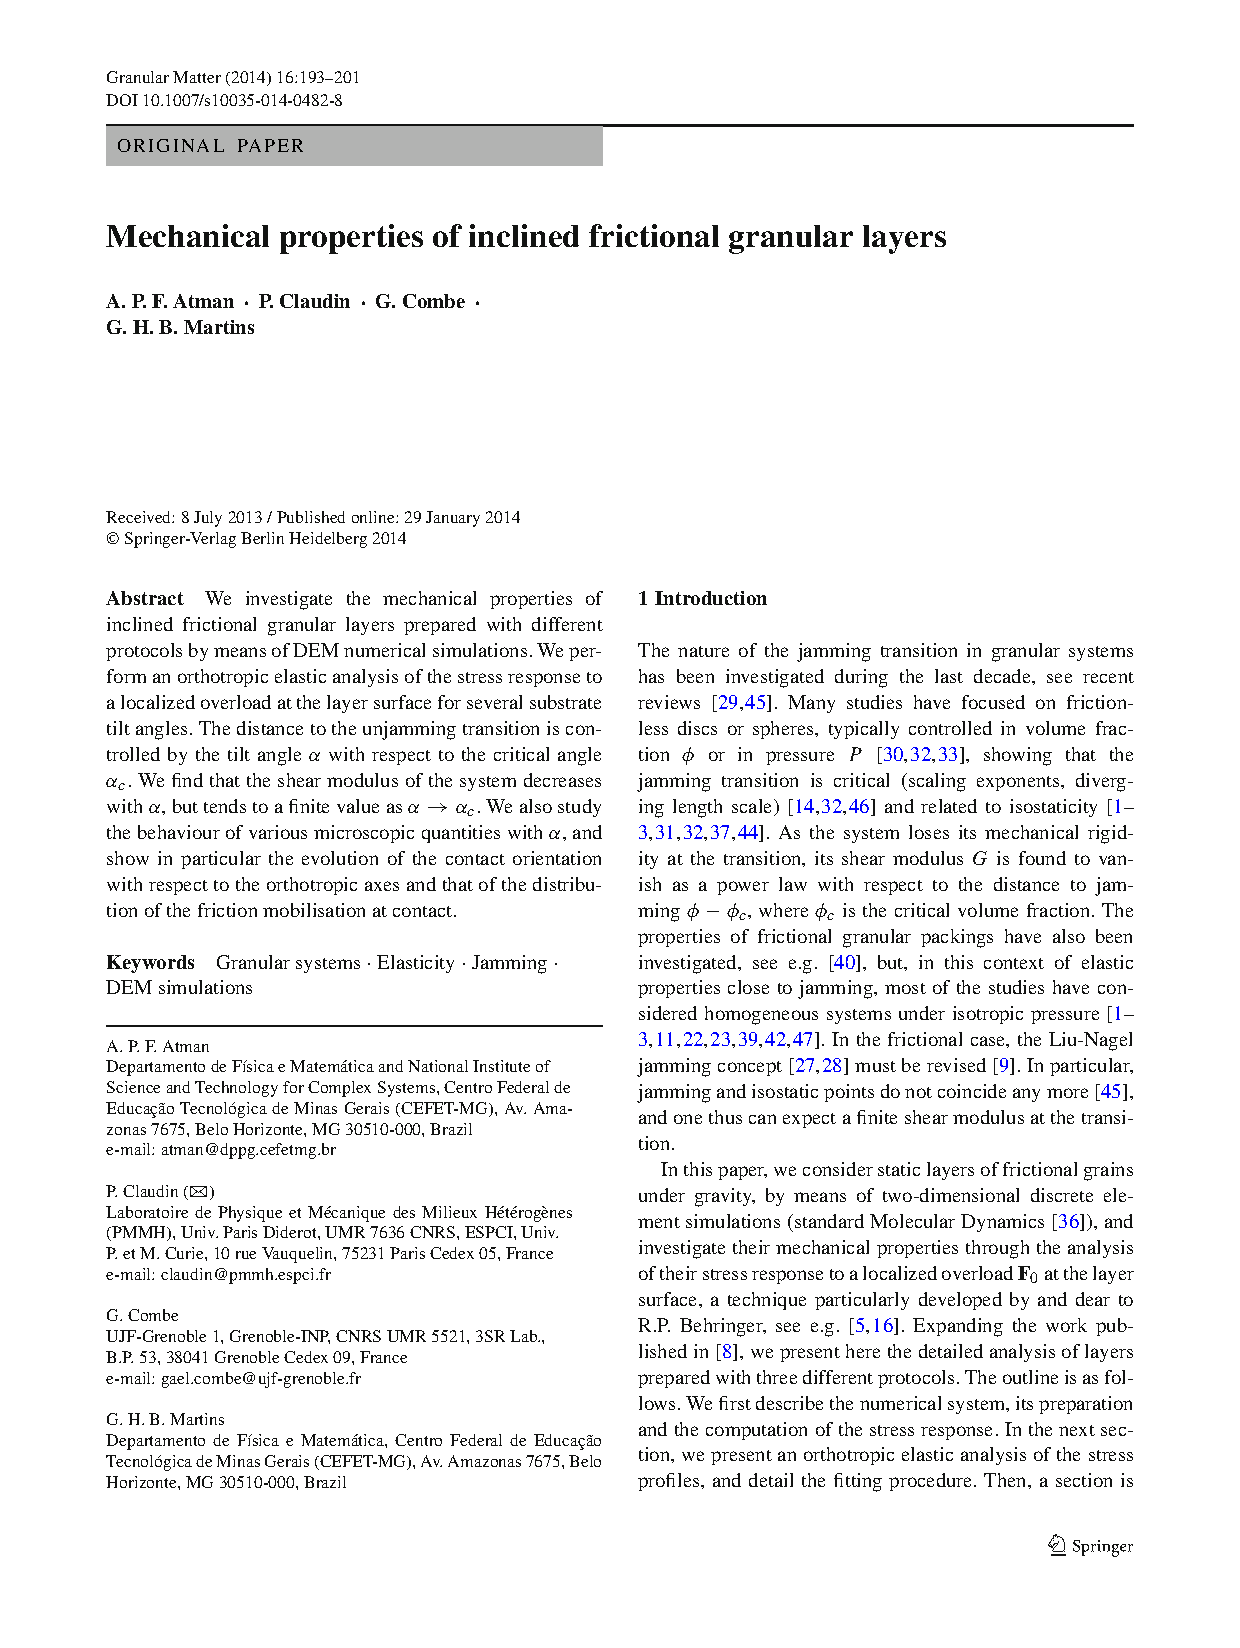
\includepdf[pages=-]{./08-apendice/ArtigoGM.pdf}

\section{\textit{Non-Gaussian behavior in jamming / unjamming transition in dense granular materials}}

    Este artigo foi publicado no quatrienal do congresso \textit{Powders \& Grains 2013}, que é o maior congresso sobre materiais granulares, e que estava em sua 7ª edição.

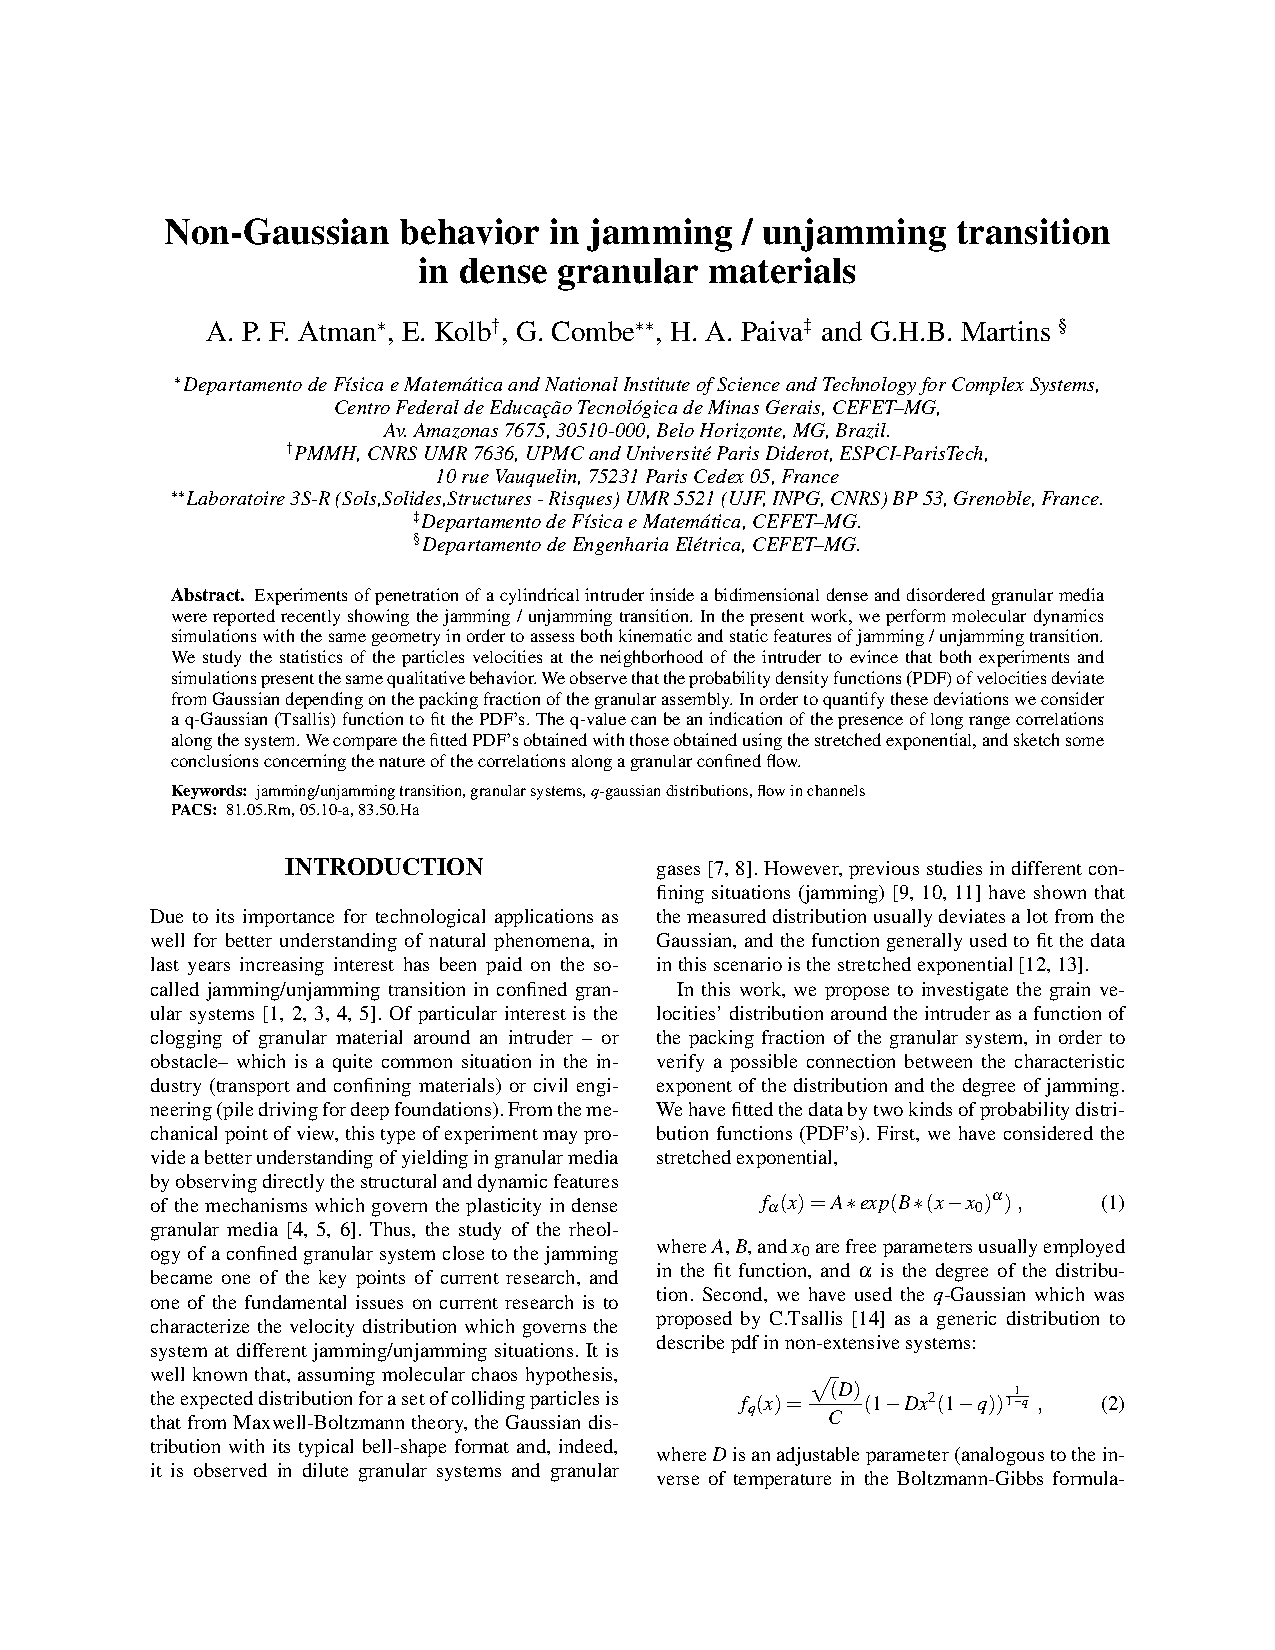
\includepdf[pages=-]{./08-apendice/ArtigoPG2013.pdf}

\chapter{Códigos}

    Coloquei os códigos utilizados para este projeto de tese em um GIT para a maior comodidade e facilidade do acesso. O endereço eletrônico é \url{https://github.com/BoscoWarhammer/Doutorado}.

\end{apendicesenv}
             % Apêndices
%% -----------------------------------------------------------------------------
% Anexos
% -----------------------------------------------------------------------------

\begin{anexosenv}
\partanexos

% -----------------------------------------------------------------------------
% Primeiro anexo
% -----------------------------------------------------------------------------

\chapter{Nome do anexo}     % edite para alterar o título deste anexo
\label{chap:anexoA}

Lembre-se que a diferença entre apêndice e anexo diz respeito à autoria do texto e/ou material ali colocado.

Caso o material ou texto suplementar ou complementar seja de sua autoria, então ele deverá ser colocado como um apêndice. Porém, caso a autoria seja de terceiros, então o material ou texto deverá ser colocado como anexo.

Caso seja conveniente, podem ser criados outros anexos para o seu trabalho acadêmico. Basta recortar e colar este trecho neste mesmo documento. Lembre-se de alterar o "label"{} do anexo.

Organize seus anexos de modo a que, em cada um deles, haja um único tipo de conteúdo. Isso facilita a leitura e compreensão para o leitor do trabalho. É para ele que você escreve.

% -----------------------------------------------------------------------------
% Novo anexo
% -----------------------------------------------------------------------------

\chapter{Dica: nomes no BibTeX}
\label{chap:anexoB}

Se você utiliza LaTeX para a redação de artigos já deve ter se deparado com algum tipo de problema no modo como o nome dos autores é apresentado no documento final (pior é quando a "descoberta"{} ocorre depois de já ter submetido o paper). Muitas vezes é difícil encontrar uma maneira certa de escrever o nome no arquivo *.bib e garantir que ele seja transcrito corretamente independente do estilo utilizado. Este texto tem o intuito de discutir o modo como o BibTeX interpreta o nome dos autores e ajudar na árdua tarefa de organizar a bibliografia.

Pessoalmente eu prefiro fornecer o nome completo dos meus autores para o BibTeX, sem abreviações e sem omitir nomes, quando possível. Desse modo, eu dou garantia que a minha bibliografia irá conter todos os dados para referenciar o autor independente do estilo utilizado para apresentá-lo. Depois disso, eu simplesmente espero que o BibTeX faça a abreviação e a colocação dos nomes da maneira correta de acordo com o estilo indicado. No entanto, para que essa tarefa seja feita é preciso apresentar os nomes da maneira correta para que a sua divisão seja feita de forma apropriada.

Para entender como o BibTeX divide um nome, é preciso conhecer antes as diversas partes que podem compor o nome de uma pessoa, que, a princípio, são: primeiro nome, nome do meio, ligação, último nome e júnior. A descrição de cada uma dessas partes é feita a seguir.

\begin{itemize}
    \item \textbf{Primeiro nome:} é o nome da pessoa, geralmente utilizado para identificar uma pessoa em um contexto informal. Ex.: Diego, João, Maria etc. Em alguns casos o primeiro nome pode ser composto por dois nomes, como Maria Ana, Victor Hugo, etc. Nestes casos, deve-se observar como a pessoa utiliza o nome para poder diferenciar a segunda parte como Primeiro nome ou Nome do meio.

    \item \textbf{Nome do meio:} é o nome que sucede o primeiro nome, mas antecede o último nome, geralmente abreviado, por simplicidade. Ex.: Alan Mathison Turing, "Mathison"{} é o nome do meio. É comum uma pessoa possuir mais do que um nome do meio e também é comum que o nome do meio de alguns autores seja desconhecido, devido às abreviações e omissões feitas pelo mesmo.

    \item \textbf{Ligação:} também chamado de separador, são as palavras "de"{}, "da"{}, "do"{}, "e"{}, "von"{}, entre outras que ligam um nome ao outro. Em John von Neumann e Ricardo Luis de Azevedo da Rocha, por exemplo, as palavras "von"{}, "de"{}  e "da"{}  são as ligações. Num contexto geral, elas normalmente são grafadas com inicial minúscula para não serem confundidas com o nome do meio e, embora não seja comum em todos lugares do mundo, no Brasil é comum um nome possuir até mais do que uma ligação.

    \item \textbf{Último nome:} também chamado de nome de família, é o nome utilizado para identificar uma pessoa em situações formais, como referência em artigos, livros etc. Ex.: Albert Einstein, "Einstein"{} é o último nome.

\item \textbf{Júnior:} é um sufixo do nome que indica a existência de um parente com o mesmo nome. Geralmente abreviado como "Jr."{} pode ser apresentado de diversas formas como "Filho"{}, "Neto"{} ou traduzido para o idioma de origem do dono do nome, como "fils"{} (filho) em francês. Ex.: John Forbes Nash Jr.
\end{itemize}

Quando indicamos o nome de um autor no BibTeX ele interpreta os nomes seguindo uma das três regras a seguir:

\begin{enumerate}
    \item \textbf{Nenhuma vírgula:} {Primeiro nome} {ligação} {Último nome}

    \item \textbf{Uma vírgula:} {ligação} {Último nome}, {Primeiro nome}

    \item \textbf{Duas vírgulas:} {ligação} {Último nome}, {Júnior}, {Primeiro nome}
\end{enumerate}

Como pode-se notar, a distinção entre essas três possíveis interpretações se dá com base na quantidade de vírgulas que foram inseridas e no posicionamento da ligação, que devem sempre ser escritas com a inicial minúscula. O(s) nome(s) do meio são todos os nomes que estão após o primeiro nome, porém antes da ligação e do último nome. A princípio, o BibTeX interpreta os nomes do meio como sendo parte do primeiro nome.

Para mostrar como isso pode gerar problemas, imagine, por exemplo, se o nome "John Forbes Nash Jr."{} fosse apresentado em um arquivo BibTeX. Como nenhuma vírgula foi inserida, será entendido que "John Forbes Nash"{} é o primeiro nome e "Jr."{} é o último nome, o que não seria correto. De forma semelhante, se for apresentado na forma "Nash Jr., John Forbes", então "John Forbes"{} será o primeiro nome enquanto "Nash Jr."{} será o último nome, que também está incorreto.

Portanto, a maneira correta de referenciar seria utilizando a terceira opção pois é a única que inclui o Jr. (utilizando duas vírgulas): "Nash, Jr., John Forbes"{}, fazendo com que "John Forbes"{} seja compreendido como primeiro nome, "Nash"{} como último nome e "Jr."{} como o júnior.

Outro grande problema ocorre quando um nome possui mais do que uma ligação, como em "Ricardo Luis de Azevedo da Rocha"{}. Quando o BibTeX lê um nome como esse, ele entende que tudo que vem após o ligador, faz parte do último nome. Neste caso, "Ricardo Luis"{} seria tratado como o primeiro nome e "Azevedo da Rocha"{} como último nome.

Para evitar esse comportamento, devemos optar pela segunda opção (utilizando uma vírgula), ou seja, "da Rocha, Ricardo {Luis de} Azevedo"{}, fazendo com que o último nome seja somente "Rocha"{} e precedido pelo seu ligador.

Note que neste último exemplo o ligador e o nome que o antecede foram delimitados por chaves. Este é um pequeno e útil truque que pode ser feito para garantir que os ligadores não sejam inclusos ao abreviar nomes (Ex.: Universidade de São Paulo, abrevia-se U.S.P. ao invés de U. de S.P. ou U.d.S.P.). Fazendo isso, o BibTeX passa a tratar "Luis de"{} como um único nome e o abrevia corretamente quando necessário.

E qual a importância de garantir que o BibTeX interprete corretamente as diversas partes de um nome? A verdade é que cada estilo trata o nome de uma maneira diferente: o IEEE, por exemplo, coloca apenas as iniciais do primeiro nome e a ligação seguida do último nome; a Nature, por outro lado, coloca a ligação e o último nome, seguido das iniciais do primeiro nome; e assim por diante. Assim sendo, entender como os nomes são interpretados nos ajuda a garantir que o mesmo seja sempre dividido da maneira correta e formatado apropriadamente independente do estilo fornecido.

Por fim, e não menos importante, também deixo aqui um aviso sobre a acentuação no BibTeX. Eu já presenciei diversos problemas com relação a acentuação nos nomes dos autores, títulos dos artigos etc. Em especial os problemas ocorreram quando eu estava utilizando o abnTeX, que é um projeto que tem o objetivo de implementar o padrão ABNT em formato TeX. Embora este projeto não seja um dos mais ativos, ele ainda é muito utilizado e alguns grupos de pesquisa utilizam estilos que nada mais são do que versões derivadas deste (como é o caso do laboratório que faço parte).

O problema é que este estilo possui uma falha (descrita em \href{http://abntex.codigolivre.org.br/node5.html}{http://abntex.codigolivre.org.br}), que impede que acentos sejam convertidos corretamente em letras maiúsculas. Para contornar o problema eles pedem que sejam utilizados códigos para descrever os acentos nos arquivos *.bib ao invés de inseri-los diretamente pelo teclado. Dado a quantidade de problemas que essa falha me gerou, julgo isso como uma boa prática e deixo aqui a minha recomendação de que não sejam utilizados caracteres não-ASCII nos arquivos *.bib.

Como os arquivos *.bib são interpretados pelo LaTeX, é possível utilizar alguns comandos em seus campos. A saber, segue os comandos para formar os acentos mais comuns:
\\
\\
\\

[A parte final do texto original foi suprimida, por conter incorreções.]\footnote{Nesta parte era apresentado os comandos \LaTeX{} para acentuação. No entanto, foi constatado que os comandos, se utilizados como apresentado, provocariam erros na transformação de minúsculas para maiúsculas e vice-versa, algo bastante recorrente no estilo \texttt{abntex2}. Para a tabela com os comandos corretos veja \autoref{fig:acentos-latex}.}.
\\
\\
\\

[Em \href{http://en.wikibooks.org/wiki/LaTeX/Special_Characters}{http://en.wikibooks.org/wiki/LaTeX/Special\underline{ }Characters}] você encontra diversos outros acentos e símbolos para serem utilizados no LaTeX.

Referência:\\

Alexander Binder. Help On BibTeX Names. Disponível em <\href{www.kfunigraz.ac.at/~binder/texhelp/bibtx-23.html}{www.kfunigraz.ac.at/...}>. Acessado em 4 de março de 2011.

\end{anexosenv}
                % Anexos
% -----------------------------------------------------------------------------
% Índice Remissivo
% -----------------------------------------------------------------------------

% -----------------------------------------------------------------------------
% Este comando gera automaticamente o índice remissivo para os termos definidos
% no corpo do documento
% -----------------------------------------------------------------------------

\printindex

% -----------------------------------------------------------------------------
% Este arquivo não necessita de ser editado.
% -----------------------------------------------------------------------------
      % Índice Remissivo

\end{document}
